\documentclass[12pt]{article}

\usepackage{booktabs}% http://ctan.org/pkg/booktabs
\usepackage[utf8]{inputenc}
\usepackage{changepage}
\usepackage{pgfplots}
\usepackage{amssymb}
\usepackage{xcolor}
\usepackage{hyperref}
\usepackage{listings}
\usepackage[T1]{fontenc}
\usepackage[utf8]{inputenc}
\usepackage{adjustbox}
\usepackage{amsmath}
\usepackage{mathtools}
\usepackage{biblatex}

\lstset{
  language=Python,
  numbers=left,
  numberstyle=\tiny,
  stepnumber=1,
  numbersep=5pt,
  tabsize=4,
  basicstyle=\ttfamily,
  columns=fullflexible,
  keepspaces,
}
\hypersetup{
    colorlinks,
    citecolor=black,
    filecolor=black,
    linkcolor=black,
    urlcolor=black
}

% Set page size and margins
% Replace `letterpaper' with `a4paper' for UK/EU standard size
\usepackage[letterpaper,top=2cm,bottom=2cm,left=3cm,right=3cm,marginparwidth=1.75cm]{geometry}

% Useful packages
\usepackage{amsmath}
\usepackage{mathtools}
\usepackage{graphicx}
\newenvironment{para}{\begin{adjustwidth}{13mm}{}}{\end{adjustwidth}}

\newcommand\tab[1][1cm]{\hspace*{#1}}

\newcommand{\tabitem}{\llap{\textbullet}}
\newcommand{\Hsquare}{%
\text{\fboxsep=-.2pt\fbox{\rule{0pt}{1ex}\rule{1ex}{0pt}}}%
}

\newtheorem{Definizione}{Definizione}[subsection]
\newtheorem{Lemma}{Lemma}[subsection]
\newtheorem{Teorema/Definizione}{Teorema/Definizione}[subsection]
\newtheorem{Corollario}{Corollario}[subsection]
\newtheorem{Teorema}{Teorema}[subsection]
\newtheorem{Proposizione}{Proposizione}[subsection]
\newtheorem{Notazione}{Notazione}[subsection]
\newtheorem{Commento}{Commento}[subsection]
\newtheorem{Dimostrazione}{Dimostrazione}[subsection]
\newtheorem{Osservazione}{Osservazione}[subsection]
\newtheorem{Nota}{Nota}[subsection]

\title{Ricerca operativa e pianificazione delle risorse}
\author{spitfire}
\date{A.A. 2023-2024}
\begin{document}
\begin{figure}
    \centering
    
\includegraphics[width=0.35\textwidth]{Images/Logo scienze bicocca.png}
\end{figure}

\vspace{10cm}
\date{A.A. 2024-2025}


\maketitle

\newpage

\tableofcontents
\newpage

\section{Prerequisiti di Algebra Lineare}
\subsection{Matrici e vettori}
Una matrice è una tabella contenente numeri.
Se la tabella è costituita da $m$ righe e $n$ colonne si parla
di una matrice  $m \times n$. 
Una matrice viene detta \textbf{matrice quadrata} se il numero di righe
e colonne coincidono. \newline
Una matrice $1 \times m$ viene detto \textbf{vettore riga m-dimensionale} \newline
Una matrice $m \times 1$ viene detto \textbf{vettore colonna m-dimensionale}. \newline
La notazione maggiormente utilizzata per indicare una matrice è
$$A = [a_{ij}]$$
Con $a_{ij}$ elemento generico della i-esima riga e j-esima colonna della matrice $A$.
Se $A = [a_{ij}]$ è una matrice $m \times n$, la matrice $n \times m$
$$A^T=[a_{ij}]$$
viene detta \textbf{matrice trasposta} della matrice $A$.

Se $A = [a_{ik}]$ è una matrice $m \times p$ e $B = [b_{kj}]$ è una matrice $p \times n$ la loro
\textbf{matrice prodotto} è $m \times n$ e definita come:
$$A \cdot B = C = [c_{ij}] \; con \; c_{ij} = \sum_{k = 1}^{p} a_{ik} \cdot b_{kj}$$
Date due matrici $m \times n, A = [a_{ij}]$ e $B = [b_{ij}]$, la loro \textbf{matrice somma} è definita come segue:
$$A+B=C=[c_{ij}] \; con \; c_{ij} = a_{ij} + b_{ij}$$
La \textbf{moltiplicazione} di una \textbf{matrice A per una costante $\alpha$} fornisce come risultato quanto segue:
$$\alpha \cdot A = [\alpha \cdot a_{ij}]$$
Questa moltiplicazione è \textbf{commutativa}. \newline
Siano $v_1, v_2, ..., v_n$ n vettori, riga o colonna; essi vengono detti
\textbf{linearmente indipendenti} tra loro se, prendendo $n$ coefficienti $a_1, a_2, ..., a_n$ la seguente uguaglianza
$$a_1 \cdot v_1 + a_2 \cdot v_2 + ... + a_n \cdot v_n = 0$$
risulta verificata solo se $a_1 = a_2 = ... = a_n = 0$. \newline
Al contrario, se esistono coefficienti $a_1, a_2, ..., a_n$ non tutti nulli per cui
$$a_1 \cdot v_1 + a_2 \cdot v_2 + ... + a_n \cdot v_n = 0$$
i vettori $v_1, v_2, ..., v_n$ sono detti \textbf{linearmente dipendenti}. \newline
Un insieme di $n$ vettori ad $n$ dimensioni linearmente indipendenti costituisce una \textbf{base per uno spazio a n dimensioni}.
Se un insieme di vettori $v_1, v_2, ..., v_n$ costituisce una base per uno spazio ad $n$ dimensioni, allora ogni vettore $x$ che appartiene
a quello spazio è \textbf{combinazione lineare dei vettori della base}. \newline
Una matrice quadrata $m \times m$ si dice \textbf{matrice singolare} se l'insieme degli $m$ vettori riga (o colonna), ottenuti considerando
ogni riga (o colonna) come un vettore, è \textbf{linearmente dipendenti}.
Se, viceversa, l'insieme degli $m$ vettori è linearmente indipendente, la matrice si dice \textbf{matrice non singolare}. \newline
Una matrice quadrata $A = [a_{ij}]$ con $a_{ij} = 0$ per ogni $i \neq j$ viene detta \textbf{matrice diagonale}. \newline
La matrice diagonale $A = [a_{ij}]$, con $a_{ii} = 1$ per ogni $i$ viene detta \textbf{matrice identità}, solitamente indicata con $I$.
Se $A$ NON è una matrice singolare, allora esiste una matrice $A^{-1}$ detta \textbf{matrice inversa} della matrice $A$, tale per cui vale la
seguente relazione di uguaglianza:
$$A \cdot A^{-1} = A^{-1} \cdot A = I$$
Il \textbf{determinante} di una matrice quadrata $A$ si indica con $det(A)$ ed è un numero (esiste solo per matrici quadrate), nel caso
specifico di una matrice $2 \times 2$ si definisce come segue:
$$det(A) = det\begin{pmatrix}
    a_{11} & a_{12} \\
    a_{21} & a_{22}
\end{pmatrix} = a_{11} \cdot a_{22} - a_{12} \cdot a_{21}$$
Il determinante di una matrice quadrata $A$ $m \times m$ si ottiene utilizzando la seguente regola ricorsiva, detta \textbf{formula di Laplace}:
Se $A_{ij}$ è la matrice $(m-1) \times (m-1)$, ottenuta togliendo la i-esima riga e la j-esima colonna di A, il determinante di A risulta:
$$det(A) = \sum_{j=1}^{m} (-1)^{i+j} \cdot a_{ij} \cdot det(A_{ij}) \; (formula \; per \; righe)$$
$$det(A) = \sum_{i=1}^{m} (-1)^{i+j} \cdot a_{ij} \cdot det(A_{ij}) \; (formula \; per \; colonne)$$
Se la matrice è singolare, allora $det(A) = 0$. \newline
Una matrice quadrata $A$ ammette inversa se e solo se non è singolare.
\subsection{Equazioni lineari}
Un' \textbf{equazione lineare} nelle variabili $x_1, x_2, ..., x_n$ è un'equazione nella seguente forma:
$$a_1 \cdot x_1 + a_2 \cdot x_2 + ... + a_n \cdot x_n = b$$
dove $a_1, a_2, ..., a_n$ e $b$ sono delle costanti.
Si dice \textbf{soluzione dell'equazione} un qualsiasi vettore $|y_1, y_2, ..., y_n| \in \mathbb{R}^n$ tale che:
$$a_1 \cdot y_1 + a_2 \cdot y_2 + ... + a_n \cdot y_n = b$$
Un \textbf{sistema di m equazioni lineari in n variabili} è definito come segue:
$$\begin{cases}
    a_{11} \cdot x_1 + a_{12} \cdot x_2 + ... + a_{1n} \cdot x_n = b_1 \\
    a_{21} \cdot x_1 + a_{22} \cdot x_2 + ... + a_{2n} \cdot x_n = b_2 \\
    ... \\
    a_{m1} \cdot x_1 + a_{m2} \cdot x_2 + ... + a_{mn} \cdot x_n = b_m
\end{cases}$$
dove $a_{ij}$ e $b_{j}$, $i = 1,...,n$; $j = 1,...,m$ sono costanti.
Una \textbf{soluzione del sistema lineare} è un qualsiasi vettore $|y_1, y_2, ..., y_n| \in \mathbb{R}^n$ tale che le $m$ equazioni
del sistema lineare siano contemporaneamente soddisfatte.
Trovare le soluzioni del sistema lineare equivale a individuare il punto di intersezione tra le sue equazioni, ammesso che un tale punto esista. \newline
Un sistema di equazioni lineari può essere:
\begin{itemize}
    \item \textbf{Consistente}: se ammette almeno una soluzione, in caso contrario viene detto \textbf{inconsistente}
    \item \textbf{Determinato}: se costituito da un numero di equazioni uguale al numero di incognite $m = n$. Un tale sistema ha \textbf{una sola soluzione}
    \item \textbf{Sovradeterminato}: se costituito da più equazione che incognite $m>n$. Un tale sistema è spesso, ma non sempre, inconsistente
    \item \textbf{Sottodeterminato}: se costituito da meno equazioni che incognite $m<n$. Un tale sistema ammette infinite soluzioni
\end{itemize}
Consideriamo la forma matriciale del sistema costituito da $m$ equazioni lineari in $n$ incognite
$$A \cdot x = b$$
dove
\begin{itemize}
    \item $A$ è una matrice $m \times n$ (nota)
    \item $x$ è un vettore colonna in $n$ dimensioni (incognito)
    \item $b$ è un vettore colonna in $m$ dimensioni (noto)
\end{itemize}
Si definisce \textbf{rango della matrice A} come segue:
\begin{itemize}
    \item \textbf{Rango di riga}: numero massimo di righe linearmente indipendenti
    \item \textbf{Rango di colonna}: numero massimo di colonne linearmente indipendenti
\end{itemize}
Se $rango \; di \; riga = rango \; di \; colonna$ allora $rk(A) \leq min(m, n)$ \newline
Se $rk(A) = min (m, n)$, allora la matrice A viene detta \textbf{a rango pieno}. \newline
Data la matrice dei coefficienti $A$, si dice \textbf{matrice aumentata} la matrice $C = A,b$ ottenuta
dalla matrice $A$ aggiungendo come colonna aggiuntiva il vettore dei termini noti $b$.
Avremo quanto segue:
\begin{itemize}
    \item $rk(C) > rk(A)$: Il sistema lineare non ammette soluzione
    \item $rk(C) = rk(A)$: il sistema lineare ammette soluzione
\end{itemize}
Assumiamo $rk(C) = rk(A)$, allora:
\begin{itemize}
    \item Caso $m \geq n$
    \begin{itemize}
        \item Se $rk(A) = n$, allora il sistema ha una soluzione unica
        \item Se $rk(A) < n$, allora il sistema ha infinite soluzioni
    \end{itemize}
    \item Caso $m < n$
    \begin{itemize}
        \item Se $rk(A) \leq m$, allora il sistema ha infinite soluzioni
    \end{itemize}
\end{itemize}
Come si risolve un sistema di equazioni lineari? Abbiamo due metodi:
\subsubsection{Metodo di eliminazione}
Procediamo come segue:
\begin{enumerate}
    \item Selezionare una variabile, e risolvere una delle equazioni rispetto ad essa e eliminare
    la variabile in questione dalle altre equazioni
    \item Tralasciare l'equazione utilizzata nel passo di eliminazione e tornare al passo 1)
    \item Applicare il processo di \textbf{Back-walk substitution}: dall'ultima equazione, tornare indietro e risolvere le restanti
\end{enumerate}
\subsubsection{Metodo di eliminazione di Gauss}
Il metodo di eliminazione di Gauss è un metodo di eliminazione che utilizza solo le operazioni elementari su matrici, cioè:
\begin{itemize}
    \item Moltiplicare una riga per uno scalare non nullo
    \item Sommare una riga moltiplicata per uno scalare non nullo con un'altra riga
    \item Permutare le righe 
\end{itemize}
\begin{Teorema}
    Applicare operazioni elementari a un sistema di equazioni lineari non cambia l'insieme delle sue soluzioni.
\end{Teorema}
\section{Prerequisiti di Analisi Matematica}
\subsection{Funzioni di una variabile}
Si dice \textbf{funzione} una terna $(A, B, f)$ con:
\begin{itemize}
    \item $A, B$ due insiemi non vuoti
    \item $f$ una legge che ad ogni elemento $x \in A$ associa uno ed uno solo elemento $f(x) \in B$
\end{itemize}
dove:
\begin{itemize}
    \item $A$ è detto dominio della funzione $f$, anche indicato con $dom(f)$
    \item $B$ è detto codominio della funzione $f$
    \item Scriviamo $f: A \rightarrow B$ e $x \in dom(f) \rightarrow f(x)$, per indicare la legge che alla variabile indipendente $x$ associa la sua immagine $f(x)$
\end{itemize}
Data una funzione $f: A \rightarrow B$, se esiste, finito o meno, il limite:
$$\lim_{h \rightarrow 0} \frac{f(x_0 + h) - f(x_0)}{h} = \frac{f(x) - f(x_0)}{x - x_0}$$
esso viene chiamato \textbf{derivata della funzione f nel punto $x_0$} e viene indicato con
$$f'(x_0) = \frac{d}{dx}f(x_0)$$
Se $f'(x_0) \in \mathbb{R}$, allora $f$ si dice derivabile in $x_0$. \newline
\newpage
Riportiamo le derivate elementari:
\begin{itemize}
    \item Se $f(x) = c, \forall x \in \mathbb{R}$ allora $f'(x) = 0, \forall x \in \mathbb{R}$
    \item Se $f(x) = x^n, n \in \mathbb{N}, n \geq 2$ allora $f'(x) = n \cdot x^{n-1}, \forall x \in \mathbb{R}$
    \item Se $f(x) = \frac{1}{x}, \forall x \in \mathbb{R}^+$ allora $f'(x) = -\frac{1}{x^2}, \forall x \in \mathbb{R}^+$
    \item Se $f(x) = log(x), x \in \mathbb{R}^+$ allora $f'(x) = \frac{1}{x}, \forall x \in \mathbb{R}^+$
\end{itemize}
Data una funzione $f: \mathbb{R} \rightarrow \mathbb{R}$ e un punto $x_0 \in \mathbb{R}$, allora
\begin{itemize}
    \item $f$ derivabile in $x_0 \Rightarrow f$ continua in $x_0$
    \item $f$ continua in $x_0 \not\Rightarrow f$ derivabile in $x_0$
\end{itemize}
Se $f, g: \mathbb{R} \rightarrow \mathbb{R}$ sono derivabili in $x_0 \in \mathbb{R}$, allora
\begin{itemize}
    \item $\forall c \in \mathbb{R}$, la funzione $c \cdot f$ è derivabile in $x_0$ e $(c \cdot f)'(x_0) = c \cdot f'(x_0)$
    \item La funzione $f + g$ è derivabile in $x_0$ e $(f+g)'(x_0) = f'(x_0) + g'(x_0)$
\end{itemize}
Se $f, g: \mathbb{R} \rightarrow \mathbb{R}$ sono derivabili in $x_0 \in \mathbb{R}$, allora anche la funzione $f \cdot g$ è derivabile
in $x_0$ e si ha quanto segue
$$(f \cdot g)'(x_0) = f'(x_0) \cdot g(x_0) + f(x_0) \cdot g'(x_0)$$
Date due funzioni $f, g: \mathbb{R} \rightarrow \mathbb{R}$, con $f$ derivabile in $x_0 \in \mathbb{R}$ e $g$ derivabile in
$f(x_0)$, allora $g \circ f$ è derivabile in $x_0$ e si ha quanto segue:
$$(g \circ f)'(x_0) = g'(f(x_0)) \cdot f'(x_0)$$
La derivata della \textbf{derivata prima $f'$} in $x_0 \in \mathbb{R}$ viene detta \textbf{derivata seconda} e indicata come $f''(x_0)$. \newline
La derivata è il \textbf{coefficiente angolare} della retta tangente alla funzione nel punto di derivazione $x_0$. \newline
Data una funzione $f(x)$ definita su un intervallo chiuso $[a,b]$ diremo che la funzione è:
\begin{itemize}
    \item \textbf{Crescente}: nell'intervallo $[a,b]$ quando per ogni coppia di punti $x_1, x_2 \in [a,b]$ con $x_1 < x_2$ risulta che $f(x_1) < f(x_2)$
    \item \textbf{Decrescente}: nell'intervallo $[a,b]$ quando per ogni coppia di punti $x_1, x_2 \in [a,b]$ con $x_1 < x_2$ risulta che $f(x_1) > f(x_2)$
\end{itemize}
Per determinare se la funzione $f:[a,b] \rightarrow \mathbb{R}$ sia crescente o decrescente in un punto $x_0 \in [a,b]$ è possibile ricorrere alla valutazione della sua derivata
nel punto $x_0$, infatti:
\begin{itemize}
    \item Se $f'(x_0) >0$ allora è crescente nel punto considerato $x_0$
    \item Se $f'(x_0) <0$ allora la funzione è decrescente nel punto considerato $x_0$
\end{itemize}
Una funzione $f:[a,b] -> \mathbb{R}$ si dice \textbf{convessa} se $\forall x_1, x_2 \in [a,b]$ con $x_1 < x_2$ vale la seguente relazione
$$f(x) \leq f(x_1) + \frac{f(x_2) - f(x_1)}{x_2 - x_1} \cdot (x - x_1) \; \forall x \in [a,b]$$
\textbf{strettamente convessa} se:
$$f(x) < f(x_1) + \frac{f(x_2) - f(x_1)}{x_2 - x_1} \cdot (x - x_1) \; \forall x \in [a,b]$$
Una funzione $f:[a,b] -> \mathbb{R}$ si dice \textbf{concava} se $\forall x_1, x_2 \in [a,b]$ con $x_1 < x_2$ vale la seguente relazione
$$f(x) \geq f(x_1) + \frac{f(x_2) - f(x_1)}{x_2 - x_1} \cdot (x - x_1) \; \forall x \in [a,b]$$
\textbf{strettamente concava} se:
$$f(x) > f(x_1) + \frac{f(x_2) - f(x_1)}{x_2 - x_1} \cdot (x - x_1) \; \forall x \in [a,b]$$
Data una funzione continua $f:[a,b] \rightarrow \mathbb{R}$ possiamo affermare che
\begin{itemize}
    \item Essa è crescente (decrescente) in un punto $x \in [a,b]$ se la sua derivata prima è positiva (negativa) in $x$
    \item I \textbf{punti di stazionarietà} (estremanti) della funzione sono i punti in cui la derivata prima della funzione $f$ si annulla cambiando di segno,
    nello specifico si ha un punto di \textbf{massimo} in $x \in [a,b]$ quando $f'$ passa da un valore \textbf{positivo} a un valore \textbf{negativo}, mentre si ha un punto di
    \textbf{minimo} in $x \in [a,b]$ quando $f'$ passa da un valore $negativo$ a un valore $positivo$
    \item È detta \textbf{lineare} se la sua \textbf{derivata prima è una funzione costante}
\end{itemize}
\begin{center}
    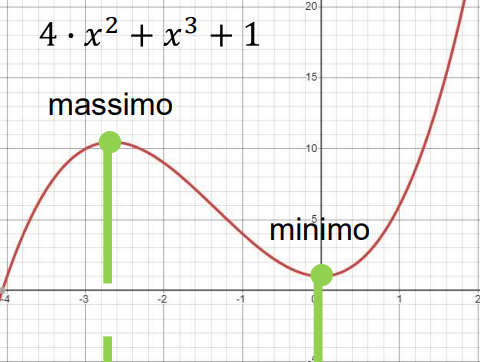
\includegraphics[width = 0.50\textwidth]{Images/1.PNG}
\end{center}
Data una funzione continua $f:[a,b] \rightarrow \mathbb{R}$ e un punto $x_0 \in [a,b]$, si dice che $f$ ha un minimo o massimo locale (o relativo) nel punto 
$x_0$ quando esiste un intorno $l(x_0)$ nel quale risulta
\begin{itemize}
    \item $f(x) \geq f(x_0) \forall x \in l(x_0)$ allora $x_0$ è un \textbf{minimo locale}
    \item $f(x) \leq f(x_0) \forall x \in l(x_0)$ allora $x_0$ è un \textbf{massimo locale}
    \item $x_0$ è un \textbf{minimo locale relativo} se la funzione è decrescente immediatamente a sinistra di $x_0$ e crescente immediatamente a destra
    \item $x_0$ è un \textbf{massimo locale relativo} se la funzione è crescente immediatamente a sinistra di $x_0$ e decrescente immediatamente a destra 
\end{itemize}
Il punto minimo (massimo) locale in cui la funzione $f$ assume il valore minimo (massimo) viene detto \textbf{minimo} (\textbf{massimo}) \textbf{globale} o \textbf{assoluto}.
\subsection{Funzioni in due o più variabili}
Una funzione continua definita come $f: \mathbb{R} \times \mathbb{R} \rightarrow \mathbb{R}$ che associa ad ogni coppia di numeri reali $(x_1, x_2) \in \mathbb{R} \times \mathbb{R} = R^2$ uno
e un solo valore $y \in \mathbb{R}$ viene detta \textbf{funzioni in due variabili} $(x_1, x_2)$, che vengono dette \textbf{variabili indipendenti}, mentre la variabile $y$ viene riferita con il termine di
\textbf{variabile dipendente}.
Questo concetto è generalizzabile al caso in cui si considerino $n$ variabili indipendenti $(x_1, x_2, ..., x_n) \in \mathbb{R}^n$. In questo caso
si parla di funzione $f: \mathbb{R}^n \rightarrow \mathbb{R}$ in $n$ variabili indipendenti, funzione che descrive una "regola" per ottenere dall'insieme delle $n$ variabili indipendenti $(x_1, x_2, ..., x_n)$ un singolo
valore reale di $y$. \newline
Una funzione in $n$ variabili $f: \mathbb{R}^n \rightarrow \mathbb{R}$ viene detta \textbf{funzione lineare} nelle variabili $(x_1, x_2, ..., x_n)$ se è nella forma:
$$f(x_1, x_2, ..., x_n) = a_0 + a_1 \cdot x_1 + a_2 \cdot x_2 + ... + a_n \cdot x_n$$
dove $a_0, a_1, ..., a_n$ sono parametri che assumono valore reale. \newline
Una funzione in $n$ variabili $f: \mathbb{R}^n \rightarrow \mathbb{R}$ viene detta \textbf{funzione quadratica} nelle variabili $(x_1, x_2, ..., x_n)$ se è nella forma:
$$f(x_1, x_2, ..., x_n) = a_0 + \sum_{k=1}^n b_k \cdot x_k + \sum_{i = 1}^n \sum_{j \neq i,1}^n h_{ij} \cdot x_i \cdot x_j + \sum_{k=1}^n h_{kk} \cdot x_k^2$$
\begin{center}
    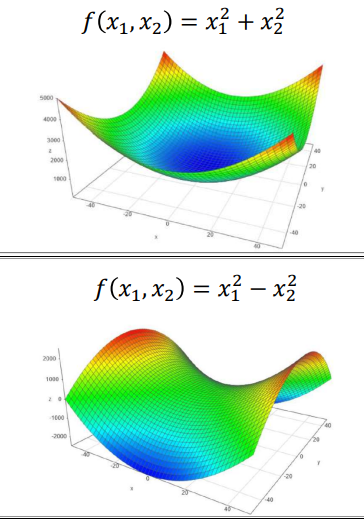
\includegraphics[width = 0.35\textwidth]{Images/2.PNG}
\end{center}
Le \textbf{curve di livello} di una funzione $f: \mathbb{R}^n \rightarrow \mathbb{R}$ sono ottenute disegnando i punti
$(x_1, x_2, ..., x_n)$ in cui la funzione ha valore constante $k$, vale a dire tutti i punti $(x_1, x_2, ..., x_n) \in \mathbb{R}^n$ per i quali vale la seguente uguaglianza
$$f(x_1, x_2, ..., x_n) = k$$
\begin{center}
    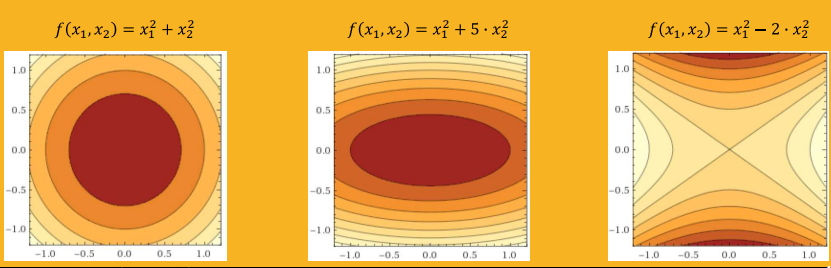
\includegraphics[width = 1\textwidth]{Images/3.PNG}
\end{center}
Dal punto di vista geometrico, le linee di livello sono le \textbf{proiezioni ortogonali} sul piano $Oxy$ delle curve ottenute
intersecando il piano $z=k$ e il grafico della funzione $z = f(x_1, x_2, ..., x_n)$
\begin{center}
    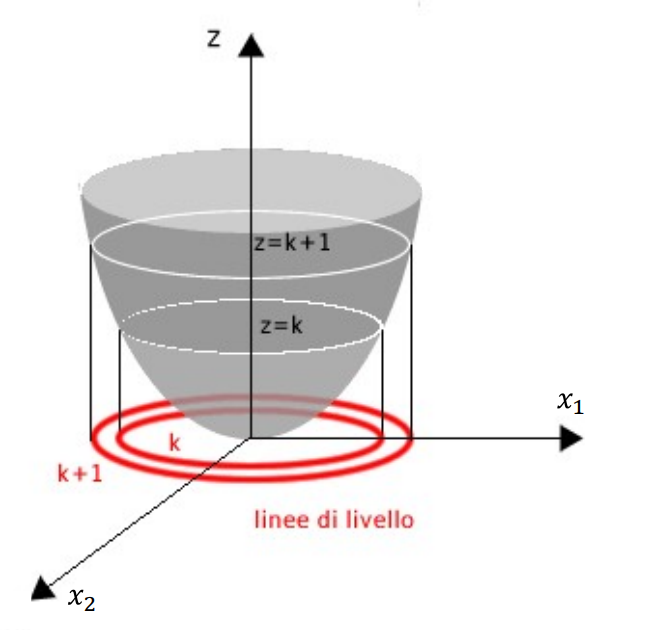
\includegraphics[width = 0.50\textwidth]{Images/4.PNG}
\end{center}
Data la funzione in 2 variabili $f: \mathbb{R}^2 \rightarrow \mathbb{R}$:
\begin{itemize}
    \item Si dice \textbf{derivata parziale rispetto a $x_1$} la seguente funzione:
    $$\frac{\partial f(x_1, x_2)}{\partial x_1} = f_{x_1} = f'_{x_1}$$
    Essa rappresenta il tasso con cui varia la funzione $f(x_1, x_2)$ al variare della variabile $x_1$, quando sia fissato e mantenuto costante
    il valore della variabile $x_2$.
    \item Si dice \textbf{derivata parziale rispetto a $x_2$} la seguente funzione:
    $$\frac{\partial f(x_1, x_2)}{\partial x_2} = f_{x_2} = f'_{x_2}$$
    Essa rappresenta il tasso con cui varia la funzione $f(x_1, x_2)$ al variare della variabile $x_2$, quando sia fissato e mantenuto costante
    il valore della variabile $x_1$
    \item Si dice \textbf{gradiente} il vettore i cui coefficienti sono le derivate parziali della funzione $f(x_1, x_2)$ rispetto alle variabili $x_1$ e $x_2$, esso è denotato nel seguente modo:
    $$\nabla f(x_1, x_2) = \begin{pmatrix}
        \frac{\partial f(x_1, x_2)}{\partial x_1} \\
        \frac{\partial f(x_1, x_2)}{\partial x_2}
    \end{pmatrix} = \begin{pmatrix}
        f'_{x_1} \\
        f'_{x_2}
    \end{pmatrix}$$
\end{itemize}
Data la funzione in 2 variabili $f: \mathbb{R}^2 \rightarrow \mathbb{R}, f(x_1, x_2)$:
\begin{itemize}
    \item Si dice \textbf{derivata parziale seconda rispetto a $x_1$} e $x_1$ la seguente funzione:
    $$\frac{\partial}{\partial x_1} \frac{\partial f(x_1, x_2)}{\partial x_1} = f_{x_1, x_1} = f'_{x_1, x_1}$$
    \item Si dice \textbf{derivata parziale seconda rispetto a $x_1$} e $x_2$ la seguente funzione:
    $$\frac{\partial}{\partial x_1} \frac{\partial f(x_1, x_2)}{\partial x_2} = f_{x_1, x_2} = f'_{x_1, x_2}$$
    \item Si dice \textbf{derivata parziale seconda rispetto a $x_2$} e $x_1$ la seguente funzione:
    $$\frac{\partial}{\partial x_2} \frac{\partial f(x_1, x_2)}{\partial x_1} = f_{x_2, x_1} = f'_{x_2, x_1}$$
    \item Si dice \textbf{derivata parziale seconda rispetto a $x_2$} e $x_2$ la seguente funzione:
    $$\frac{\partial}{\partial x_2} \frac{\partial f(x_1, x_2)}{\partial x_2} = f_{x_2, x_2} = f'_{x_2, x_2}$$
\end{itemize}
In particolare:
$$\frac{\partial}{\partial x_1} \frac{\partial f(x_1, x_2)}{\partial x_2} = f_{x_1, x_2} = f'_{x_1, x_2} = \frac{\partial}{\partial x_2} \frac{\partial f(x_1, x_2)}{\partial x_1} = f_{x_2, x_1} = f'_{x_2, x_1}$$
Data la funzione in 2 variabili $f: \mathbb{R}^2 \rightarrow \mathbb{R}, f(x_1, x_2)$, si dice
\textbf{matrice Hessiana} la matrice quadrata delle derivate parziali:
$$H = \begin{pmatrix}
    f_{x_1, x_1} & f_{x_1, x_2} \\
    f_{x_2, x_1} & f_{x_2, x_2}
\end{pmatrix}$$
\textbf{Condizione necessaria del primo ordine}: Data la funzione in 2 variabili $f: \mathbb{R}^2 \rightarrow \mathbb{R}, f(x_1, x_2)$, un punto
$(x_1, x_2)$ può essere un punto critico (minimo, massimo o sella) solo se il suo gradiente nel punto $(x_1, x_2)$ è nullo:
$$\nabla f(x_1, x_2) = \begin{pmatrix}
    0 \\
    0
\end{pmatrix}$$
Non ne conosciamo però la natura! (Minimo? Massimo? Sella?) \newpage
\textbf{Condizioni sufficienti del secondo ordine}:
Supponiamo che $(x_1, x_2)$ sia un punto critico di $f(x_1, x_2)$. Calcoliamo il determinante della matrice Hessiana:
$$det(H) = f_{x_1,x_1} (x_1, x_2) \cdot f_{x_2 x_2}(x_1, x_2) - (f_{x_1, x_2}(x_1, x_2))^2$$
Abbiamo i seguenti casi:
\begin{itemize}
    \item $det(H) > 0$:
    \begin{itemize}
        \item $f_{x_1, x_1} > 0 \Rightarrow (x_1, x_2)$ è un minimo relativo di $f(x_1, x_2)$
        \item $f_{x_1, x_1} < 0 \Rightarrow (x_1, x_2)$ è un massimo relativo di $f(x_1, x_2)$
    \end{itemize}
    \item $det(H) < 0 \Rightarrow (x_1, x_2)$ è un punto di sella di $f(x_1, x_2)$
\end{itemize}
Data la funzione in 2 variabili $f: \mathbb{R}^2 \rightarrow \mathbb{R}, f(x_1, x_2)$, se la sua matrice Hessiana $H$ è tale per cui
$f_{x_1, x_1} > 0$ e $det(H) > 0$ allora la funzione è \textbf{convessa}. Se la funzione è  convessa, allora ogni punto di minimo e di massimo sono
\textbf{globali} poiché ammette solamente un punto dove il gradiente si annulla
\section{Modelli nella Ricerca Operativa}
Data una funzione
$$f: \mathbb{R}^n \rightarrow \mathbb{R}$$
la chiamiamo \textbf{funzione obbiettivo}.
Un \textbf{problema di ottimizzazione} è formulabile come segue:
\begin{equation*}
    \begin{array}{rrclcl}
    \displaystyle \textrm{opt} & f(x)\\
    \textrm{s.a.} & x \in X & X \subseteq \mathbb{R}^n
    \end{array}
\end{equation*}
$X$ è detta \textbf{regione ammissibile}, cioè l'insieme delle soluzioni $x$ ammissibili dal problema. Inoltre, $\textrm{opt} \in \{\textrm{min}, \textrm{max}\}$. \newline
Se $\textrm{opt} = \textrm{min}$, allora abbiamo un \textbf{problema di minimizzazione}, altrimenti un \textbf{problema di massimizzazione}. \newline
Le variabili che indicano i vincoli ai quali è soggetto il problema sono dette \textbf{variabili decisionali} e identificano una soluzione del problema. \newline
Quindi, un problema di ottimizzazione consiste nel determinare, se esistono, uno o più punti di minimo/massimo $\textbf{x}^*$, assegnazione di valori alle variabili decisionali $\textbf{x}$, della funzione obbiettivo $f$ tra i punti
\textbf{x} che appartengono alla regione ammissibile $X$.
\begin{center}
    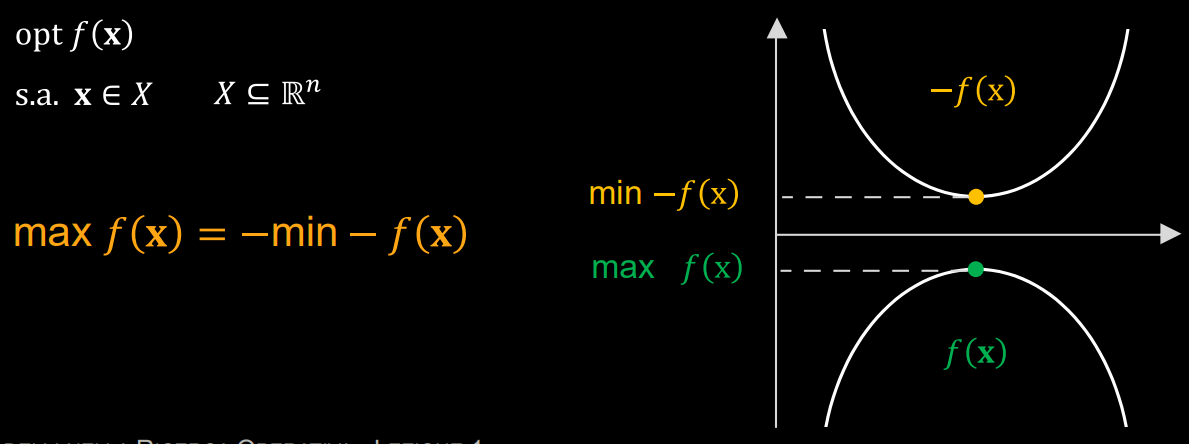
\includegraphics[width = 1\textwidth]{Images/5.PNG}
\end{center}
In particolare, se alcune zone di $\mathbb{R}^n$ non sono ammissibili, si dice che non sono \textbf{eleggibili}. \newline
Quando parliamo di ottimizzazione di una funzione obbiettivo possiamo avere diversi tipi di ottimizzazione: \newline 
\textbf{Ottimizzazione NON vincolata}: la ricerca del/i punto/i di ottimo della funzione obbiettivo viene condotta su tutto lo spazio di definizione
(quindi $X = \mathbb{R}^n)$ della/e variabile/i di decisione \newline
\textbf{Ottimizzazione vincolata}: la ricerca del/i punto/i di ottimo della funzione obbiettivo viene condotta su un sottoinsieme proprio dello spazio di definizione
(cioè $X \subset \mathbb{R}^n)$ della/e variabile/i di decisione
\textbf{Ottimizzazione intera}: le variabili di decisione assumono solo valori interi (quindi $X = \mathbb{Z}^n)$ \newline
\textbf{Ottimizzazione binaria}: Le variabili assumono solo valore 0 e 1 (quindi $X \in \{0,1\}^n$) \newline
\textbf{Ottimizzazione mista}: Alcune variabili assumono valori interi mentre altre variabili assumono solo valori binari. \newline
Se non specificato altrimenti, si deve intendere che \textbf{le variabili decisionali assumono valori reali}.
\subsection{Programmazione matematica}
Quando l'insieme $X$ delle soluzioni ammissibili di un problema di ottimizzazione viene espresso attraverso un sistema di equazione e disequazione, esso prende il nome di problema di
\textbf{programmazione matematica} (PM).
In questo caso un \textbf{vincolo} è un espressione del tipo:
$$g_i(x) \begin{Bmatrix}
    \geq \\
    = \\
    \leq
\end{Bmatrix} 0$$
Con $g_i: X \rightarrow \mathbb{R}$ funzione generica che lega tra loro le variabili decisionali.
In generale, possiamo avere uno o più vincoli. \newline
La \textbf{regione ammissibile} è quindi definita dall'insieme dei vincoli del problema, cioè:
$$X = \left \{x \in \mathbb{R}^n \; con \; g_i(x) \begin{Bmatrix} \leq \\ = \\ \geq \end{Bmatrix}, i = 1,...,m \right \}$$
Osserviamo, quindi, che abbiamo $m$ vincoli ed $n$ variabili. Inoltre
\begin{itemize}
    \item Se $x \in X$ allora $x$ è soluzione \textbf{ammissibile}
    \item Se $x \not\in X$ allora $x$ \textbf{non è una soluzione ammissibile} (soluzione inammissibile)
\end{itemize}
In un problema di ottimizzazione, abbiamo le seguenti possibilità riguardo la regione ammissibile:
\begin{itemize}
    \item \textbf{Problema non ammissibile}: $X = \emptyset$ (regione ammissibile vuota, nessuna soluzione ammissibile, problema mal posto)
    \item \textbf{Problema illimitato}, cioè:
    \begin{itemize}
        \item $\forall c \in \mathbb{R}, \exists x_c \in X | f(x_c) \leq c$ se $\textrm{opt} = \textrm{min}$ (illimitato inferiormente)
        \item $\forall c \in \mathbb{R}, \exists x_c \in X | f(x_c) \geq c$ se $\textrm{opt} = \textrm{max}$ (illimitato superiormente)
    \end{itemize}
    \item \textbf{Problema con soluzione ottima unica}
    \item \textbf{Problema con più di una soluzione ottima} (anche \textbf{infinite}): tutte le soluzione ottime hanno egual valore della funzione obbiettivo
\end{itemize}
\begin{center}
    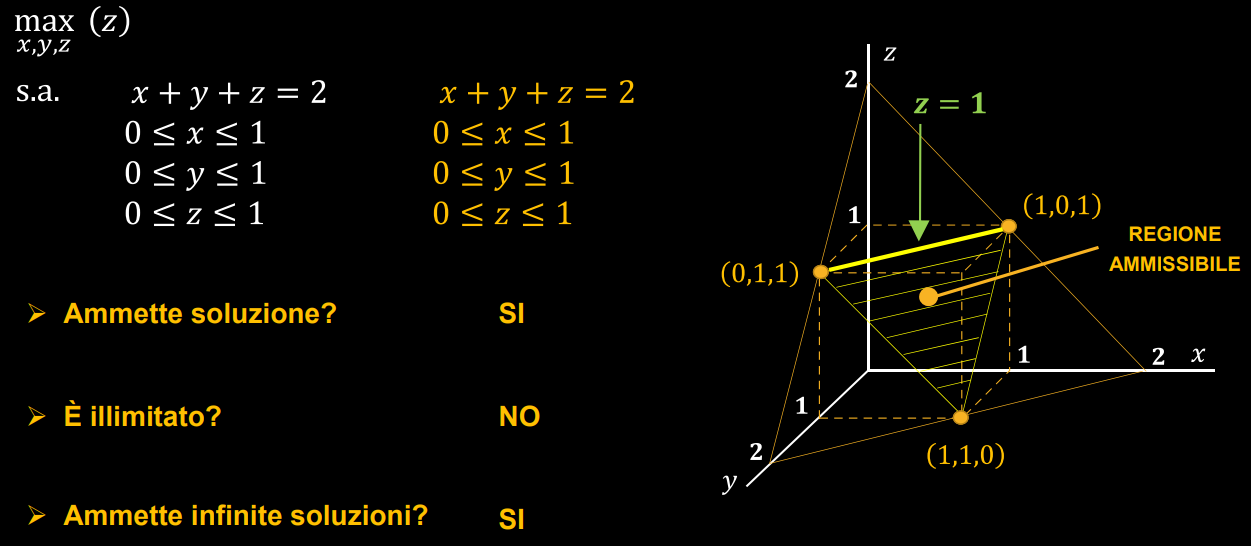
\includegraphics[width = 0.90\textwidth]{Images/6.PNG}
\end{center}
\subsection{Ottimi globali e ottimi locali}
La risoluzione di un problema di programmazione matematica consiste nel trovare una soluzione ammissibile che sia un \textbf{ottimo globale},
vale a dire un vettore $\textbf{x}^* \in X$ tale che:
\begin{itemize}
    \item $f(\textbf{x}^*) \leq f(x) \forall x \in X$ se $\textrm{opt} = \textrm{min}$
    \item $f(\textbf{x}^*) \geq f(x) \forall x \in X$ se $\textrm{opt} = \textrm{max}$
\end{itemize}
\begin{Osservazione}
    Un problema di ottimizzazione può avere:
    \begin{itemize}
        \item Più di un ottimo locale
        \item Più di un ottimo globale
    \end{itemize}
\end{Osservazione}
\begin{Osservazione}
    Un punto di ottimo globale è anche di ottimo locale
\end{Osservazione}
\begin{Osservazione}
    Nel caso di una funzione obbiettivo \textbf{convessa}, vi è un unico ottimo globale
\end{Osservazione}
Anche qui abbiamo diversi casi possibili:
\begin{itemize}
    \item \textbf{Programmazione lineare}: in questo caso ci troviamo davanti ad un problema con questa formulazione:
    $$\textrm{opt} \; f(x) = \textbf{c}^T \textbf{x} \; (lineare)$$
    La regione ammissibile è quindi formulabile in questo modo:
    $$X = \left \{x \in \mathbb{R}^n \bigg | g_i(x) \begin{Bmatrix} \leq \\ = \\ \geq \end{Bmatrix}, i = 1,...,m \right \}$$
    con $g_i(x) = \textbf{a}_j^T\textbf{x} - b_i$ vincoli \textbf{lineari}
    \item \textbf{Programmazione Lineare Intera}: in questo caso ci troviamo davanti ad un problema con questa formulazione:
    $$\textrm{opt} \; f(x) = \textbf{c}^T \textbf{x} \; (lineare)$$
    La regione ammissibile è quindi formulabile in questo modo:
    $$X = \left \{x \in \mathbb{Z}^n \bigg | g_i(x) \begin{Bmatrix} \leq \\ = \\ \geq \end{Bmatrix}, i = 1,...,m \right \}$$
    con $g_i(x) = \textbf{a}_j^T\textbf{x} - b_i$ vincoli \textbf{lineari}
    \item \textbf{Programmazione non lineare}: in questo caso ci troviamo davanti ad un problema con questa formulazione:
    $$\textrm{opt} \; f(x) \; (lineare \; o \; non \; lineare)$$
    La regione ammissibile è quindi formulabile in questo modo:
    $$X = \left \{x \in \mathbb{R}^n \bigg | g_i(x) \begin{Bmatrix} \leq \\ = \\ \geq \end{Bmatrix}, i = 1,...,m \right \}$$
    con $g_i(\textbf{x})$ vincoli \textbf{lineari} o \textbf{non lineari}. È importante notare come, in questo caso, almeno un vincolo o
    la funzione obbiettivo sono NON lineari
\end{itemize}
\section{Programmazione lineare}
La programmazione lineare (PL) è quella branca della ricerca operativa che si occupa di studiare algoritmi di risoluzione per problemi di ottimizzazione lineari.
Un problema di programmazione lineare è strutturato come segue:
$$\underset{\textbf{x} \in X}{\textrm{opt}}Z = \sum_{j=1}^{n} c_j \cdot x_j \; (Funzione \; obbiettivo \; Z \; con \; n, \; numero \; di \; variabili \; decisionali)$$
$$\sum_{j=1}^n a_{ij} \cdot x_j \leq b_i, i = 1,...,m \; (Vincoli: \; regione \; ammissibile \; X \; con \; m, numero \; di \; vincoli)$$
Con: \newline
$x_j$ \textbf{variabili decisionali} \newline
$\left. \begin{matrix}
        c_j \; \textbf{coefficienti di costo} \\
        a_{ij}\; \textbf{termini noti sinistri} \\
        b_i \; \textbf{termini noti destri} \\
\end{matrix}\right\}$ Parametri \newline
Un problema di programmazione lineare si poggia sulle seguenti \textbf{assunzioni implicite}:
\begin{itemize}
    \item \textbf{Proporzionalità}: il contributo di ogni variabile decisionale, al valore della funzione obbiettivo, è proporzionale rispetto al valore assunto dalla variabile stessa
    \item \textbf{Additività}: ogni funzione è la somma dei contributi delle variabili decisionali
    \item \textbf{Continuità}: qualunque valore delle variabili decisionali in $\mathbb{R}^n$ è accettabile
    \item \textbf{Certezza}: il valore assegnato ad ogni parametro è assunto essere noto o costante 
\end{itemize}
Vediamole nel dettaglio:
\subsection{Assunzione di Proporzionalità}
Il contributo di ogni attività al valore della \textbf{funzione obbiettivo} $Z$ è proporzionale al \textbf{livello dell'attività} $x_j$ secondo:
$$Z = \sum_{j=1}^n c_j \cdot x_j$$
Analogamente, il contributo di ogni attività al \textbf{vincolo "i"} è proporzionale al \textbf{livello di attività} $x_j$ secondo
$$\sum_{j=1}^n a_{ij} \cdot x_j \leq b_i$$
Vediamo un esempio:
\begin{center}
    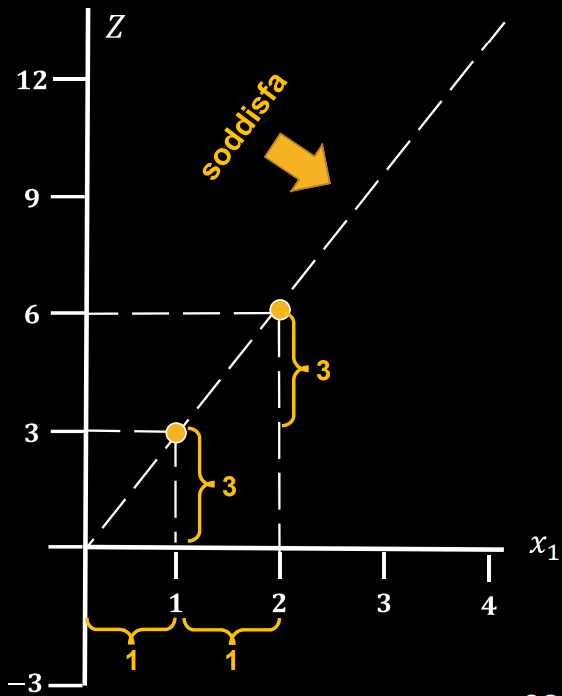
\includegraphics[width = 0.40\textwidth]{Images/7.PNG}
\end{center}
\begin{center}
    
\includegraphics[width = 0.45\textwidth]{Images/8.PNG}
\end{center}
\subsection{Assunzione di additività}
In un problema di programmazione lineare, il valore assunto da ogni funzione, sia essa \textbf{funzione obbiettivo} o vincolo, è dato dalla somma dei contributi individuali delle rispettive attività.
Vediamo un esempio:
\begin{center}
    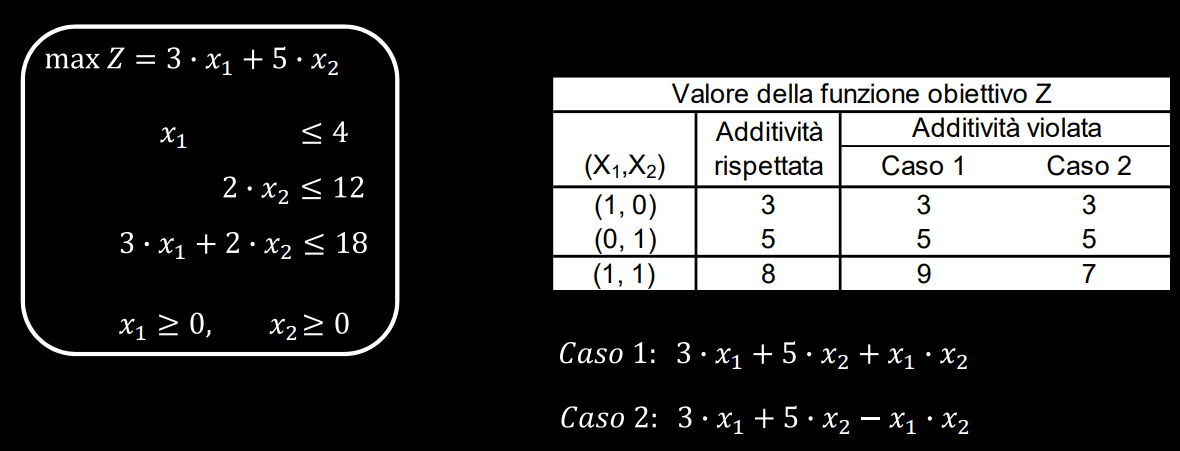
\includegraphics[width = 0.95\textwidth]{Images/9.PNG}
\end{center}
\subsection{Assunzione di continuità}
Le variabili decisionali in un problema di programmazione lineare (PL) sono libere di assumere qualsiasi valore, inclusi valori non interi che soddisfino i vincoli funzionali ed i vincoli di non negatività.
In altri termini le variabili decisionali sono continue.
In alcune condizioni può accadere che le variabili decisionali non possano che assumere valori interi; in questi casi si parla di problema di programmazione lineare intera o a numeri interi.
\subsection{Assunzione di certezza}
Il valore assegnato ad ogni parametro di un problema di programmazione lineare è assunto essere noto con certezza e costante.
\subsection{Soluzione grafica ad un problema di programmazione lineare}
Per risolvere i problemi di programmazione lineare, possiamo adottare una \textbf{procedura grafica}, determinando i valori delle variabili decisionali
$x_1, x_2$ che rispettano i vincoli, ed al tempo stesso rendono massimo il valore $Z$ della funzione obbiettivo.
La \textbf{soluzione grafica} si compone di:
\begin{itemize}
    \item Disegno della regione ammissibile
    \item Determinazione dell'ottimo
\end{itemize}
\subsubsection{Vincolo di uguaglianza}
I vincoli $g_i(\textbf{x})$ possono essere:
\begin{itemize}
    \item \textbf{Rette}: $g_i(x) = 0$
    \item \textbf{Semipiani}: $g_i(x) \leq 0$
\end{itemize}
Un vincolo del tipo $a_1 \cdot x_1 + a_2 \cdot x_2 = b$ è una \textbf{retta nel piano}.
La retta è perpendicolare al vettore $\nu = (a_1, a_2)$. Abbiamo quindi i seguenti casi:
\begin{center}
    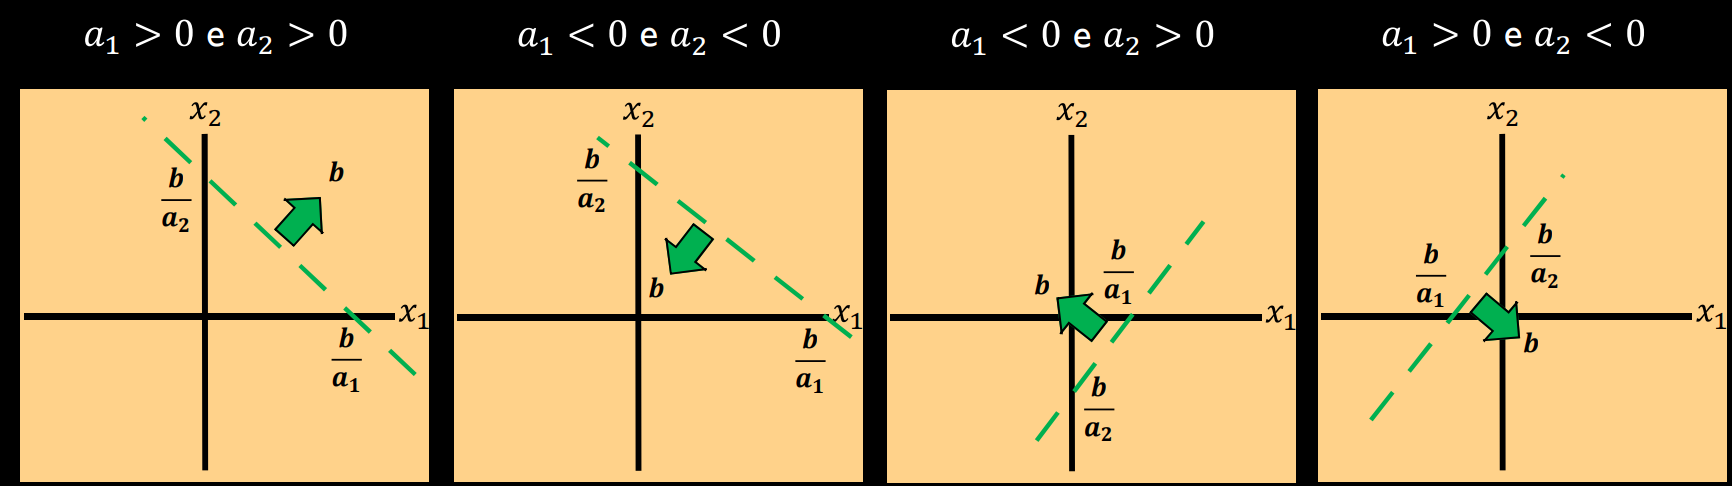
\includegraphics[width = 1\textwidth]{Images/10.PNG}
\end{center}
Come rappresentiamo però un semipiano?
\begin{enumerate}
    \item Disegniamo la retta associata $(a_1 \cdot x_1 + a_2 \cdot x_2 \leq b)$
    \item Scegliamo un punto non appartenente a tale retta (torna comodo 0)
    \begin{itemize}
        \item Se il punto verifica la disuguaglianza allora scegliamo il semipiano che lo contiene
        \item Altrimenti scegliamo l'altro semipiano
    \end{itemize}
\end{enumerate}
\begin{center}
    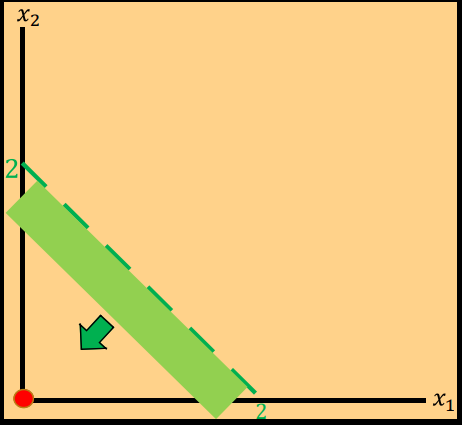
\includegraphics[width = 0.30\textwidth]{Images/11.PNG}
\end{center}
\subsubsection{Vincoli funzionali di $\leq$}
In maniera generalizzata, possiamo pensare che un problema di programmazione lineare è formulato in questo modo:
\begin{equation*}
    \begin{array}{ll}
    \displaystyle \textrm{opt} & \; Z = c_1 \cdot x_1 + c_2 \cdot x_2 +...+ c_n \cdot x_n\\
    \textrm{s.a.} & a_{11} \cdot x_1 + a_{12} \cdot x_2 +...+ a_{1n} \cdot x_n \leq b_1 \\
    \phantom{} & a_{21} \cdot x_1 + a_{22} \cdot x_2 +...+ a_{2n} \cdot x_n \leq b_2 \\
    \phantom{} &... ... ... + ... ... ... + ... + ... ... ... \leq ... \\
    \phantom{} & a_{m1} \cdot x_1 + a_{m2} \cdot x_2 +...+ a_{mn} \cdot x_n \leq b_m \\
    \phantom{} &x_1 \geq 0, x_2 \geq 0, x_3 \geq 0 ..., x_m \geq 0
    \end{array}
\end{equation*}
Con
\begin{itemize}
    \item $Z$ funzione obbiettivo
    \item $\left. \begin{matrix*}[l]
    a_{11} \cdot x_1 + a_{12} \cdot x_2 +...+ a_{1n} \cdot x_n \leq b_1 \\
    a_{21} \cdot x_1 + a_{22} \cdot x_2 +...+ a_{2n} \cdot x_n \leq b_2 \\
    ... ... ... + ... ... ... + ... + ... ... ... \leq ... \\
    a_{m1} \cdot x_1 + a_{m2} \cdot x_2 +...+ a_{mn} \cdot x_n \leq b_m \\
    \end{matrix*}\right\}$ Vincoli funzionali
    \item $x_1 \geq 0, x_2 \geq 0, x_3 \geq 0 ..., x_m \geq 0$ vincoli di non negatività
\end{itemize}
In particolare quindi:
\begin{itemize}
    \item $Z =$ valore della misura di prestazione
    \item $x_j =$ livello dell'attività j
    \item $c_j =$ incremento del valore della misura di prestazione $Z$ corrispondente all'incremento di un'unità del valore dell'attività $x_j$
    \item $b_i =$ quantità di risorsa "$i$" allocabile alle attività $x_j, j = 1,..,n$
    \item $a_{ij} =$ quantità di risorsa "$i$" consumata da ogni unità di attività $x_j, j=1,...,n$
\end{itemize}
\subsubsection{Vincoli funzionali di $\geq$ e =}
Generalizzando al caso con \textbf{$n$ variabili decisionali} ed \textbf{$m$ vincoli}, otteniamo la seguente formulazione di un \textbf{problema di programmazione lineare}: \newline
\textbf{Funzione obbiettivo}: $\textrm{opt}\; Z$ \newline
\textbf{Vincoli}:
\begin{equation*}
    \begin{array}{ll}
        a_{11} \cdot x_1 + a_{12} \cdot x_2 + ... + a_{1n} \cdot x_n \leq b_1 \\
        a_{21} \cdot x_1 + a_{22} \cdot x_2 + ... + a_{2n} \cdot x_n \geq b_2 \\
        ... \\
        a_{n1} \cdot x_1 + a_{n2} \cdot x_2 + ... + a_{nm} \cdot x_n \leq b_n \\
    \end{array}
\end{equation*}
In questo caso quindi, siamo nel caso per il quale \textbf{$x_2$ non è vincolata} da nessun valore.
Inoltre, ogni vincolo di $\geq$ e $=$ può essere riscritto nella seguente forma:
\begin{itemize}
    \item $g_i(x) \geq b_i \rightarrow -g_i(x) \leq b_i$
    \item $g_i(x) = b_i \rightarrow \begin{cases}
        g_i(x) \geq b_i \\
        g_i(x) \leq b_i
    \end{cases}$
\end{itemize}
\subsubsection{Regione ammissibile}
La regione ammissibile $X$ è data dal soddisfacimento dei vari vincoli (Rette e semipiani):
$$X = \left \{\textbf{x} \in \mathbb{R}^n \middle | g_i(x) = \begin{Bmatrix}
    \geq \\
    = \\
    \leq
\end{Bmatrix}0, i=1,...,m \right \} \; con \; g_i(x) = \textbf{a}_i^T \textbf{x} - b_i$$ 
dove $\textbf{a} \in \mathbb{R}^n, \textbf{b} \in \mathbb{R}^m$ \newline
La regione ammissibile, da un punto di vista geometrico, corrisponde ad un \textbf{poliedro convesso in $\mathbb{R}^n$}.
La regione ammissibile può essere \textbf{limitata} (\textbf{politopo}) o illimitata
\begin{center}
    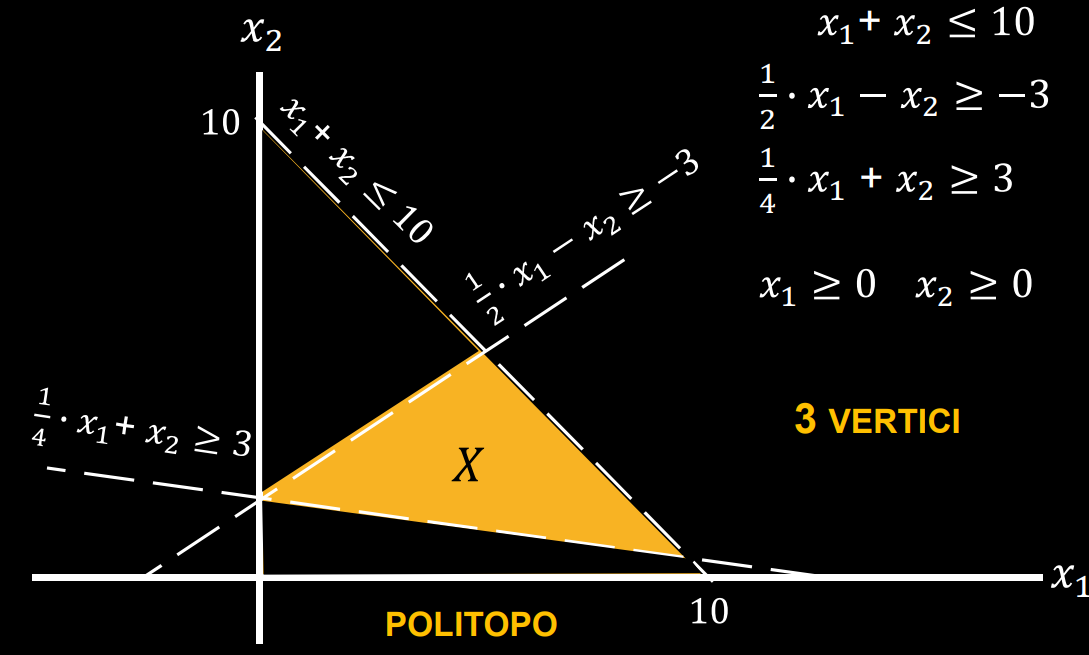
\includegraphics[width = 0.65\textwidth]{Images/12.PNG}
\end{center}
Si possono verificare quattro soluzioni:
\begin{itemize}
    \item Il problema di programmazione lineare \textbf{ammette una sola soluzione ottima} in un \textbf{vertice del poligono convesso}
    che delimita la regione ammissibile.
    \item Il problema di programmazione lineare \textbf{ammette infinite soluzioni ottime} in un \textbf{lato del poligono convesso} che delimita la regione ammissibile
    se la direzione di decrescita è perpendicolare ad un lato del poligono
    \item Il problema di programmazione lineare \textbf{ammette infinite soluzioni} perché la regione ammissibile è illimitata e la funzione obbiettivo è illimitata superiormente (se è di massimizzazione)
    o inferiormente (se di minimizzazione)
    \item Il problema di programmazione lineare \textbf{non ammette soluzione} perché la regione ammissibile è vuota
\end{itemize}
Per risolvere quindi un problema di programmazione lineare graficamente dobbiamo quindi:
\begin{enumerate}
    \item Disegnare la regione ammissibile
    \item Cercare di massimizzare (minimizzare) la soluzione, riportando ciò che troviamo sul grafico
\end{enumerate}
In particolare, per problemi in due variabili $x_1$ e $x_2$, il punto due può essere visto come segue:
\begin{center}
    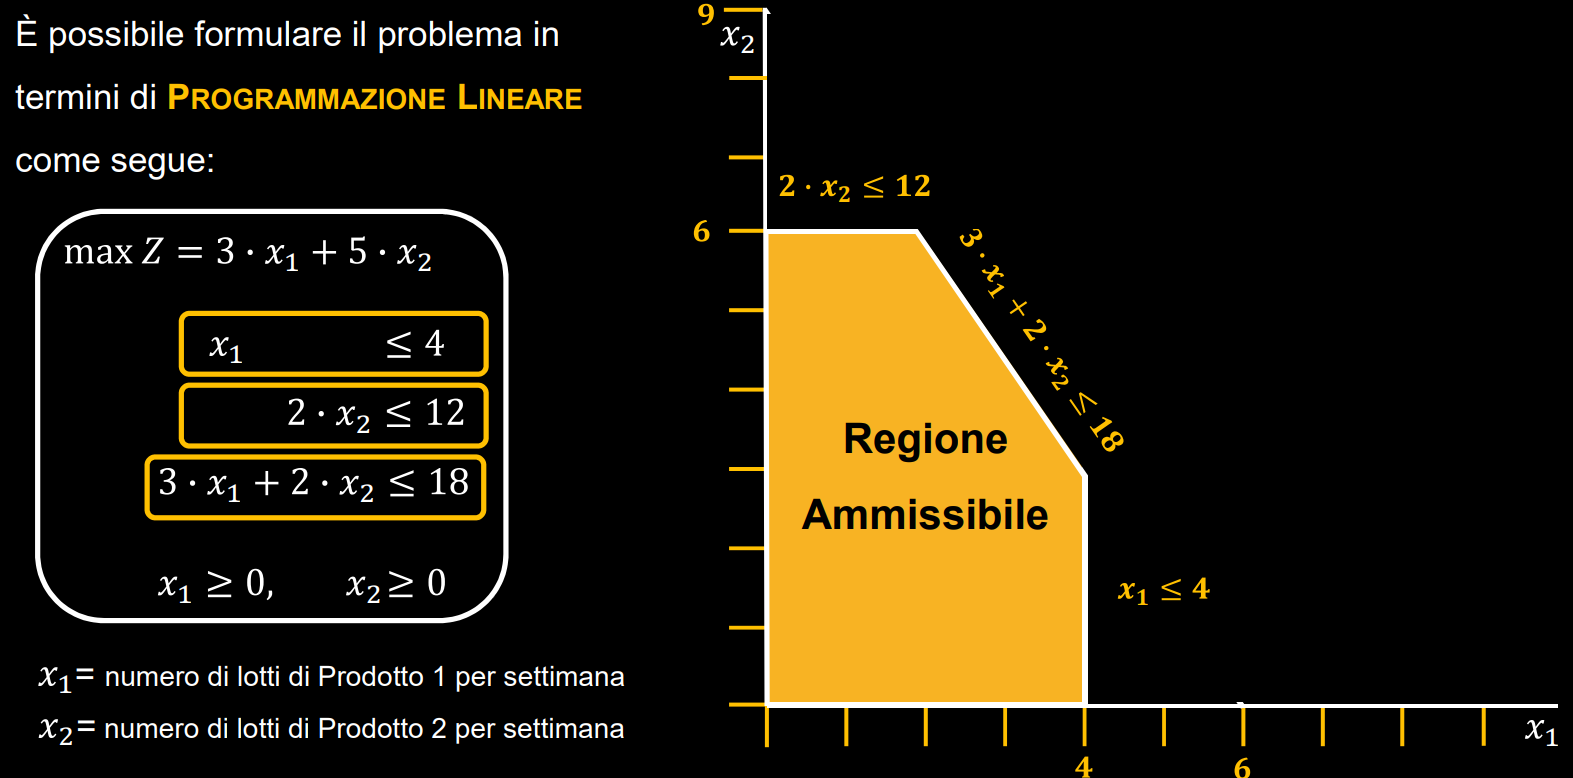
\includegraphics[width = 0.85\textwidth]{Images/13.png}
\end{center}
Riportiamo la regione ammissibile nel piano 3D e troviamo dei valori per $x_1, x_2$ che diano lo stesso valore
una volta sostituiti nella funzione obbiettivo (nell'immagine, abbiamo che i valori $x_1 = 0, x_2 = 5$ e $x_1 = 3, x_2 = 0$)
\begin{center}
    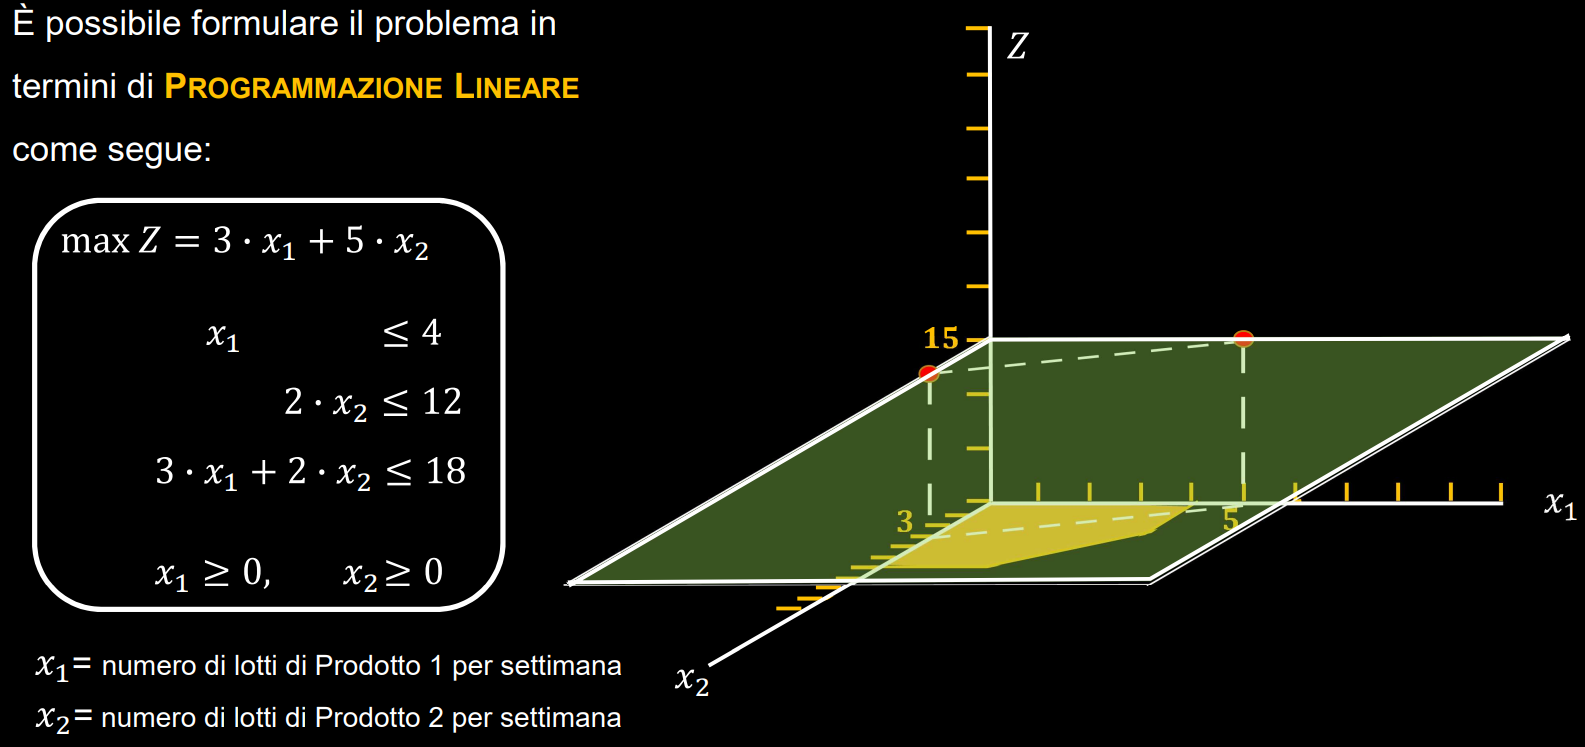
\includegraphics[width = 0.95\textwidth]{Images/14.png}
\end{center}
Continuando così, usiamo il piano creato dalla funzione obbiettivo nello spazio 3D per capire se stiamo uscendo dalla regione ammissibile o meno:
\begin{center}
    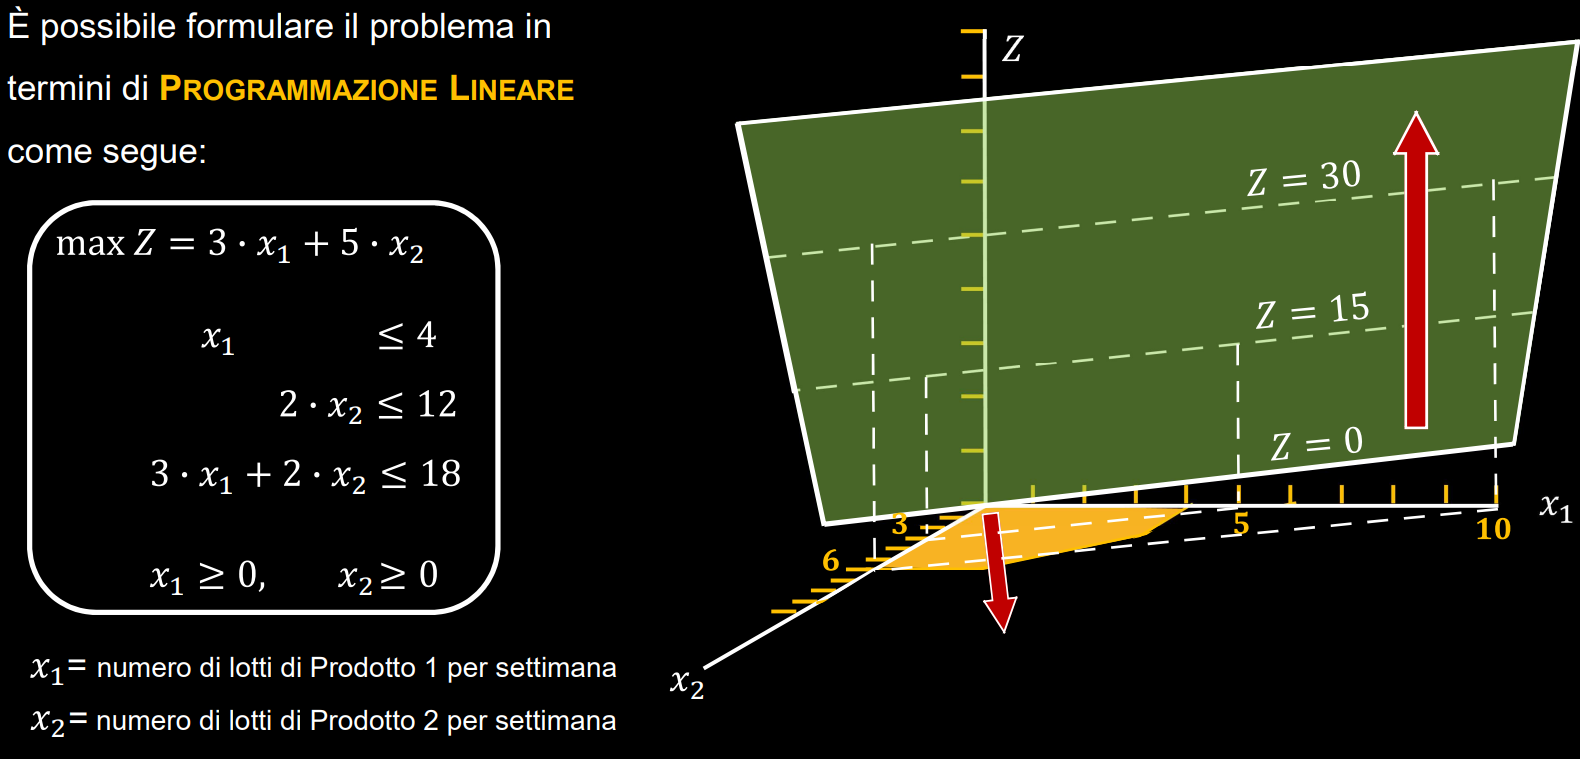
\includegraphics[width = 0.90\textwidth]{Images/15.png}
\end{center}
\begin{center}
    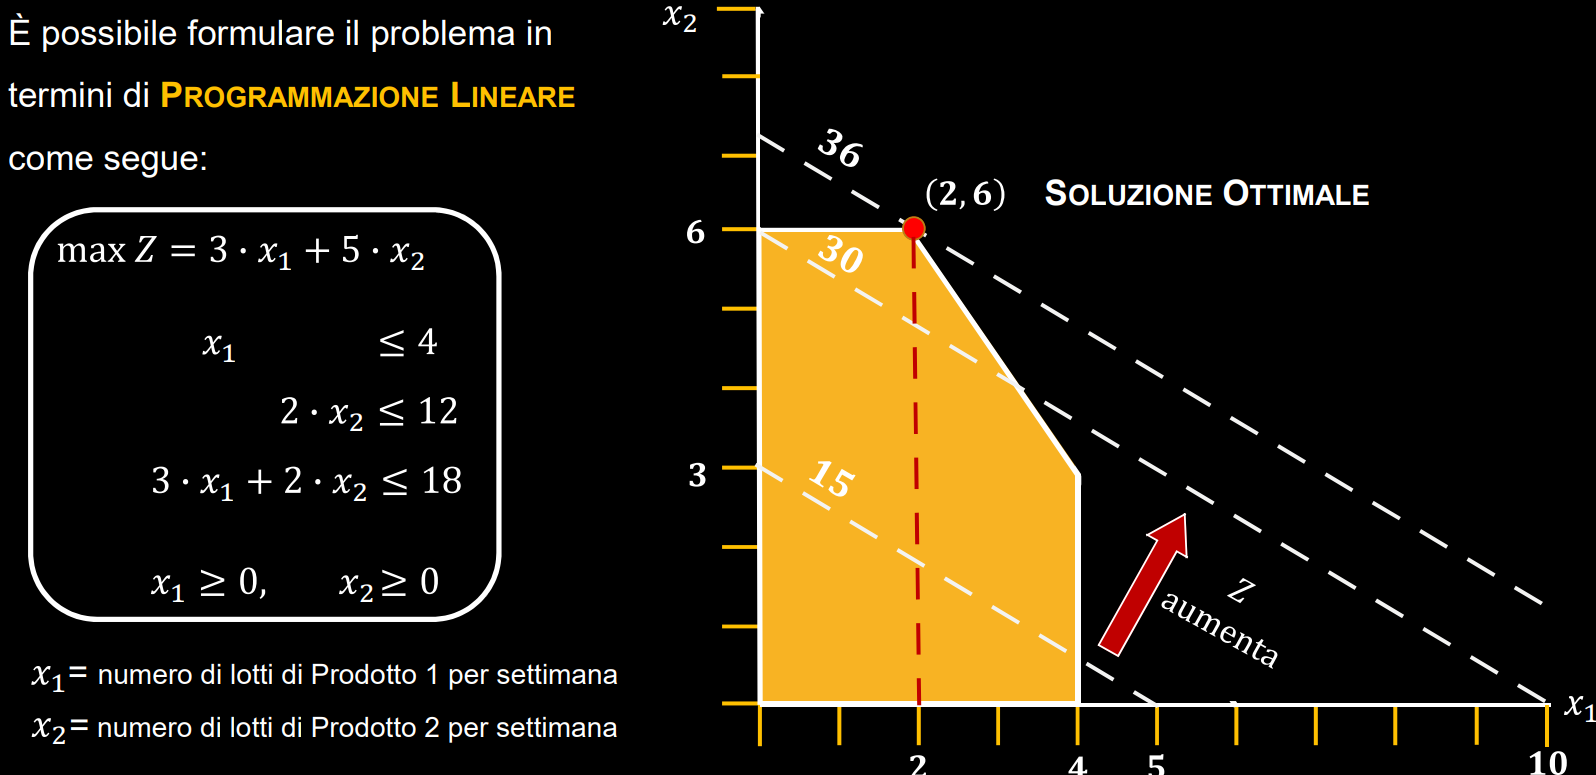
\includegraphics[width = 0.90\textwidth]{Images/16.png}
\end{center}
\subsection{Minimum cost flow problem}
Supponiamo di trovarci in questa situazione:
l'azienda \textbf{distribution unlimited} produrrà un nuovo prodotto in \textbf{due fabbriche differenti},
successivamente i prodotti verranno inviati a \textbf{due magazzini}, ogni fabbrica potrà spedire i propri prodotti ai due magazzini.
La rete distributiva è mostrata di seguito:
\begin{center}
    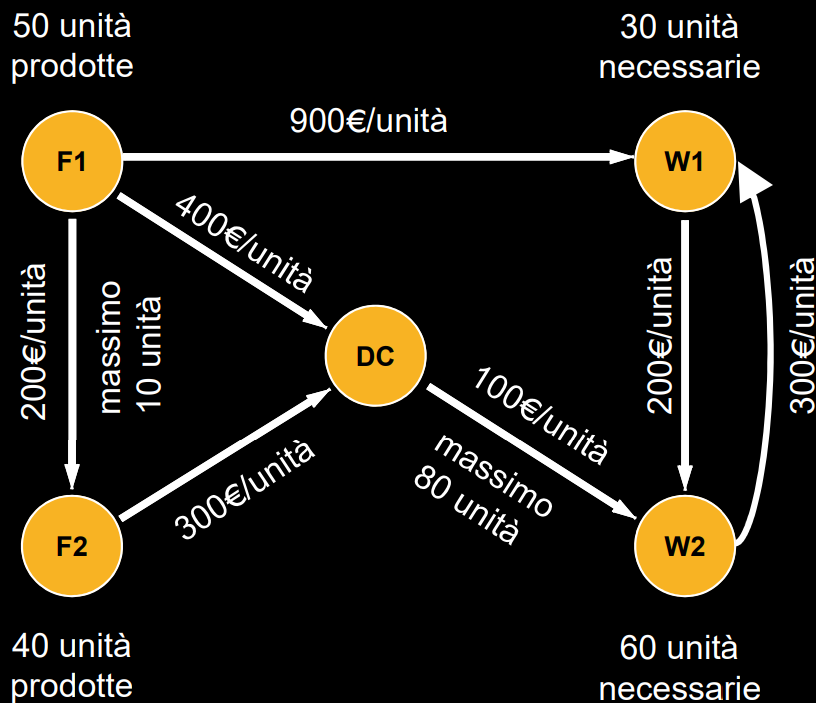
\includegraphics[width = 0.55\textwidth]{Images/17.png}
\end{center}
Il problema consiste nel determinare quante unità di prodotto spedire dalle due fabbriche \textbf{$F1$} e \textbf{$F2$} ai due magazzini
\textbf{$W1$} e \textbf{$W2$}, utilizzando anche il centro di distribuzione \textbf{$DC$}, con l'obbiettivo di \textbf{minimizzare i costi di spedizione}. \newline
Questo tipi di problema prendono il nome di \textbf{Minimum cost flow problems}. Risolviamo l'esempio come segue: \newline
Sette corsie di spedizione richiedono sette variabili decisionali:
$$x_{F1 \rightarrow F2}, x_{F1 \rightarrow W1}, x_{F1 \rightarrow DC}$$
$$x_{F2  \rightarrow DC}$$
$$x_{DC \rightarrow W2}$$
$$x_{W1 \rightarrow W2}$$
$$x_{W2 \rightarrow W1}$$
Troviamo i seguenti vincoli:
\begin{itemize}
    \item \textbf{Vincoli di non negatività}:
    \begin{equation*}
        \begin{array}{ll}
            x_{F1 \rightarrow F2}, x_{F1 \rightarrow W1}, x_{F1 \rightarrow DC} \geq 0 \\
            x_{F2  \rightarrow DC} \geq 0 \\
            x_{DC \rightarrow W2} \geq 0 \\
            x_{W1 \rightarrow W2} \geq 0  \\
            x_{W2 \rightarrow W1} \geq 0
        \end{array}
    \end{equation*}
    \item \textbf{Vincoli di capacità massima}
    \begin{equation*}
        \begin{array}{ll}
            x_{F1 \rightarrow F2} \leq 10 \\
            x_{DC \rightarrow W2} \leq 80
        \end{array}
    \end{equation*}
    \item \textbf{Vincoli di conservazione del flusso}: $outflow - inflow = unita' necessarie$ \newline
    Questo vincolo in sostanza impone che \textbf{la somma dei flussi entranti in ogni nodo deve essere pari al flusso in uscita dal nodo medesimo}
\end{itemize}
IL problema che desideriamo risolvere consiste nel determinare \textbf{quante unità di prodotto} spedire dalle due fabbriche $F1$ e $F2$ ai due magazzini
$W1$ e $W2$, utilizzando anche il \textbf{centro di distribuzione DC}, con l'obbiettivo di minimizzare il costo di spedizione. Il \textbf{costo di spedizione per unità di prodotto}
è indicato per ogni arco di spedizione.
La funzione obbiettivo è:
$$\min Z = 2 \cdot x_{F1 \rightarrow F2} + 4 \cdot x_{F1 \rightarrow DC} + 9 \cdot x_{F1 \rightarrow W1} + 3 \cdot x_{F2 \rightarrow DC} + x_{DC \rightarrow W2} + 3 \cdot x_{W1 \rightarrow W2} + 2 \cdot x_{W2 \rightarrow W1}$$
Una volta calcolati i vincoli visti sopra, possiamo risolvere il problema di programmazione lineare.
\subsection{Metodo del simplesso}
Il metodo del simplesso è un algoritmo per la risoluzione dei problemi di programmazione lineare.
Nel caso medio, il tempo computazionale dell'algoritmo è \textbf{lineare rispetto al numero di variabili}.
Nel caso peggiore, invece, può risultare \textbf{esponenziale}.
Esso è una procedura algebrica, tuttavia i suoi concetti base hanno radici geometriche.
Consideriamo la seguente regione ammissibile:
\begin{center}
    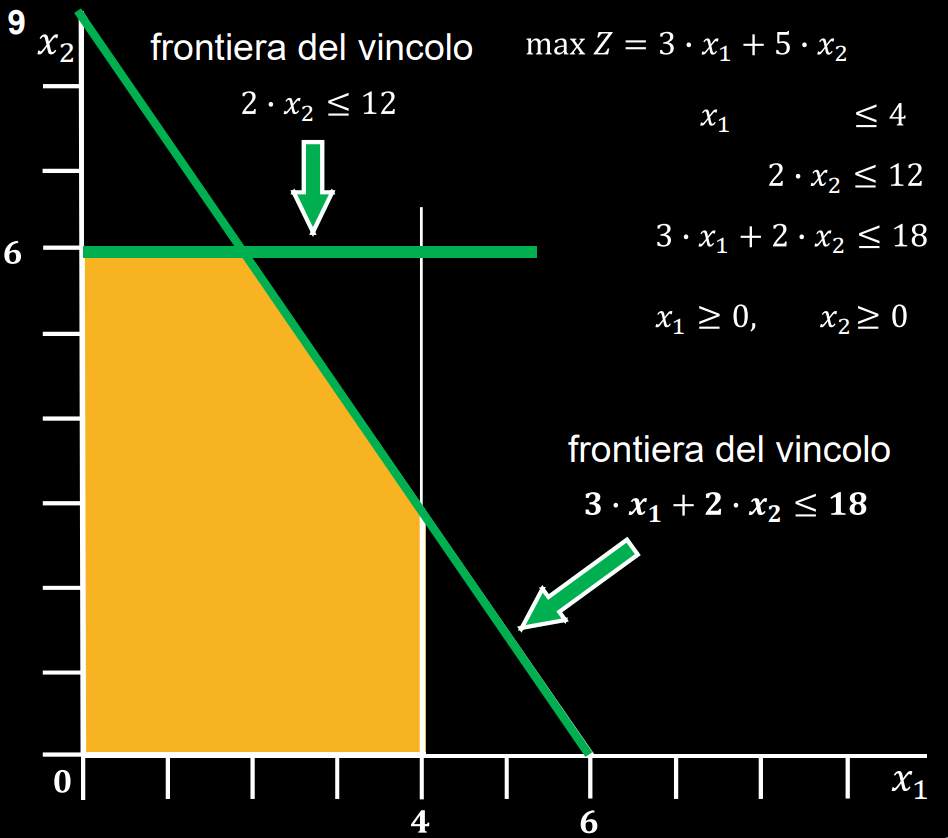
\includegraphics[width = 0.55\textwidth]{Images/18.png}
\end{center}
I \textbf{vertici} si trovano all'intersezione di coppie di frontiere di vincoli.
Per ogni problema di programmazione lineare con $n$ variabili decisionali, due vertici (soluzioni vertici)
si dicono \textbf{adiacenti} se condividono $n-1$ frontiere di vincoli.
Due vertici adiacenti sono collegati da un segmento che giace sull'intersezione delle frontiere dei vincoli condivisi.
Questo segmento viene detto \textbf{spigolo} della regione ammissibile.
\textbf{Non tutti i vertici tuttavia sono soluzioni del problema di programmazione lineare}; lo sono solamente quelli che giacciono sulla regione ammissibile.
L'interesse per i vertici adiacenti sta nella seguente proprietà di cui godono: \newline
\textbf{Test di ottimalità}: Si consideri ogni problema di programmazione lineare tale da ammettere almeno una soluzione ottimale.
Se una soluzione vertice \textbf{non ammette} soluzioni vertice a lei adiacenti con valore della funzione obbiettivo $Z$ migliore, allora la soluzione in questione è \textbf{ottimale}.
\begin{center}
    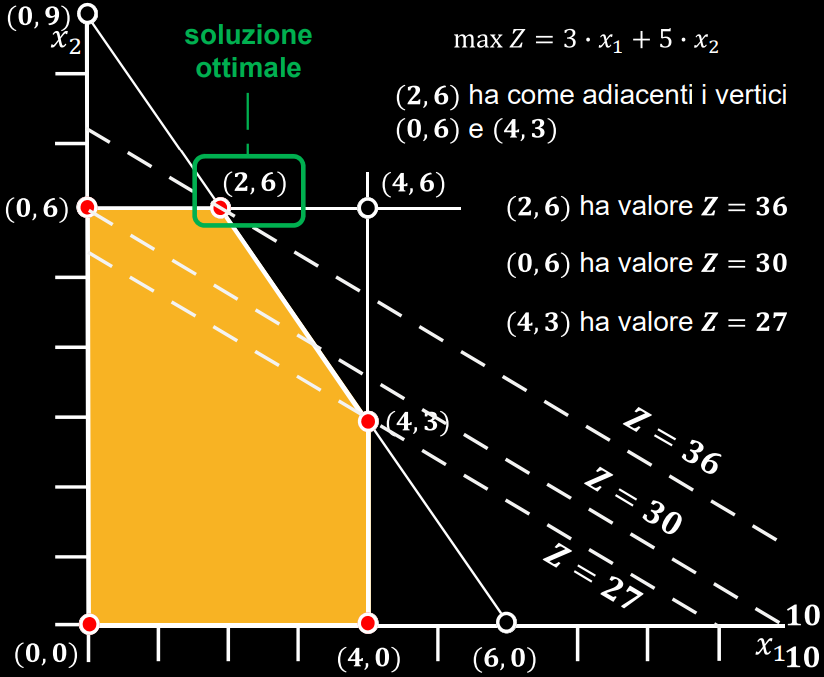
\includegraphics[width = 0.60\textwidth]{Images/19.PNG}
\end{center}
Come già detto, il metodo del simplesso è un \textbf{algoritmo} e quindi è formato da una serie di passi:
\begin{enumerate}
    \item \textbf{Inizializzazione}: Scegliere una soluzione iniziale da cui partire; possiamo sceglierne una qualunque, quindi cerchiamo in modo che sia vantaggiosa e che non richieda molte computazioni per essere identificata
    \item \textbf{Test di ottimalità}: valutiamo lo spostamento nei vertici adiacenti alla soluzione iniziale:
    \begin{itemize}
        \item Se \textbf{esiste almeno un vertice adiacente con valore della funzione obbiettivo $Z$ migliore di quello del vertice iniziale} allora ci spostiamo in quel vertice, purché esso appartenga alla regione ammissibile; in caso ci siano più vertici
        con valore della funzione obbiettivo migliore rispetto a quello iniziale, \textbf{ci spostiamo in quello che ha il valore migliore}. Ripetiamo questo passo fino a quando non troviamo vertici adiacenti con valore della funzione obbiettivo migliore rispetto al vertice in cui ci troviamo
        \item Se \textbf{non esiste almeno un vertice adiacente con valore della funzione obbiettivo $Z$ migliore di quello del vertice iniziale} allora quel vertice \textbf{è la soluzione ottimale del problema di programmazione lineare} 
    \end{itemize}
\end{enumerate}
Il metodo del simplesso si basa su \textbf{sei concetti chiave}:
\begin{itemize}
    \item \textbf{Concetto chiave 1}: Il metodo del simplesso ispeziona solo soluzioni ammissibili corrispondenti a vertici.
    \textbf{Per ogni problema di PL che ammetta almeno una soluzione ottimale, trovarne una, richiede di trovare solamente il vertice ammissibile cui compete il miglior valore della funzione obbiettivo}(La sola restrizione è che il problema possegga vertici ammissibili. Ciò è garantito dal fatto che la regione ammissibile sia limitata).
    Dato che il numero di soluzioni ammissibili è generalmente infinito, ridurre il numero di soluzioni da ispezionare ad un numero finito e piccolo è una semplificazione notevole.
    \item \textbf{Concetto chiave 2}: Il metodo del simplesso è un algoritmo iterativo con la seguente struttura:
    \begin{enumerate}
        \item \textbf{Inizializzazione}: scelta di una soluzione
        \item \textbf{Test di ottimalità}: la soluzione è ottimale?
        \begin{itemize}
            \item \textbf{NO}: torna ad 1) per trovare una soluzione migliore di quella corrente
            \item \textbf{SI}: termina l'algoritmo
        \end{itemize}
    \end{enumerate}
    \item \textbf{Concetto chiave 3}: Quando sia possibile, l'inizializzazione del metodo del simplesso seleziona l'origine (i valori di tutte le variabili di decisione vengono posti uguali a 0) come soluzione iniziale.
    \textbf{Se vi sono molte variabili decisionali, tali da rendere difficile usare il metodo grafico per scegliere la soluzione iniziale, scegliere l'origine evita di ricorrere a procedure algebriche pr determinare la soluzione iniziale del metodo del simplesso}(La soluzione nulla potrebbe però essere una soluzione non ammissibile. Se questo accade, vengono usate procedure specifiche per la scelta della soluzione iniziale)
    \item \textbf{Concetto chiave 4}: Dato un vertice, è più vantaggioso, in termini computazionali, acquisire informazioni sui vertici a lui adiacenti di quanto non sia per i vertici a lui non adiacenti. \textbf{Ad ogni iterazione, se l'algoritmo si sposta dal vertice corrente, verso un vertice con valore migliore della funzione obbiettivo, lo fa per muoversi in un vertice a lui adiacente. Nessuna altra soluzione viene considerata}.
    Pertanto, l'intero cammino, che partendo dalla soluzione iniziale raggiunge quella ottimale, attraversa spigoli della regione ammissibile
    \item \textbf{Concetto chiave 5}: A partire dal vertice corrente, il metodo del simplesso valuta i vertici ad esso adiacenti, ma non lo fa calcolando il valore della funzione obbiettivo per ognuno di essi.
    \textbf{Il metodo del simplesso valuta e compara i tassi di miglioramento della funzione obbiettivo $Z$ lungo la direzione degli spigoli che conducono dal vertice corrente ai vertici adiacenti}.
    Tra i vertici adiacenti con un tasso di miglioramento positivo per la funzione obbiettivo $Z$, il metodo del simplesso sceglie di muoversi lungo lo spigolo cui compete il massimo valore di incremento.
    \textbf{Il vertice selezionato diviene il nuovo vertice corrente}
    \item \textbf{Concetto chiave 6}: Il precedente concetto chiave descrive come il metodo del simplesso esamina gli spigoli che emanano dal vertice corrente.
    \textbf{L'ispezione di uno spigolo consente di identificare rapidamente il tasso di miglioramento di $Z$ che si otterrebbe muovendosi lungo di esso verso la soluzione adiacente all'altro estremo}.
    Un tasso di miglioramento positivo per $Z$ significa che il vertice adiacente è una soluzione migliore della soluzione corrente. Un tasso negativo implica che il vertice adiacente è una soluzione peggiore della soluzione corrente.
    \textbf{Il TEST DI OTTIMALITÀ consiste nel verificare se esiste uno spigolo con tasso positivo di miglioramento. Se tale condizione non è soddisfatta allora la soluzione corrente è ottimale}
\end{itemize}
\subsection{Procedura algebrica per il metodo del simplesso}
Fino ad ora abbiamo parlato dell'algoritmo del simplesso in termini geometrici.
Comunque, l'algoritmo del simplesso usualmente viene eseguito sun un calcolatore, il quale è in grado di interpretare solo istruzioni algebriche.
Pertanto, è necessario \textbf{tradurre la procedura geometrica in una procedura algebrica}.
La procedura algebrica si basa sulla \textbf{risoluzione di un sistema di equazioni lineari}.
Pertanto il primo passo da compiere per tradurre la procedura geometrica in procedura algebrica richiede di \textbf{tradurre i vincoli funzionali di disuguaglianza in vincoli funzionali di eguaglianza}.
I \textbf{vincoli di non negatività vengono mantenuti invariati} in quanto la loro \textbf{trattazione} viene effettuata in maniera \textbf{separata}.
Per convertire i vincoli di diseguaglianza in vincoli di uguaglianza, bisogna introdurre il concetto di \textbf{variabile slack}. \newline
Una \textbf{variabile slack} è una variabile che indica la \textbf{la quantità che manca al termine sinistro di una disuguaglianza affinche questa sia verificata con il segno di uguaglianza}.
Facciamo un esempio:
\begin{center}
    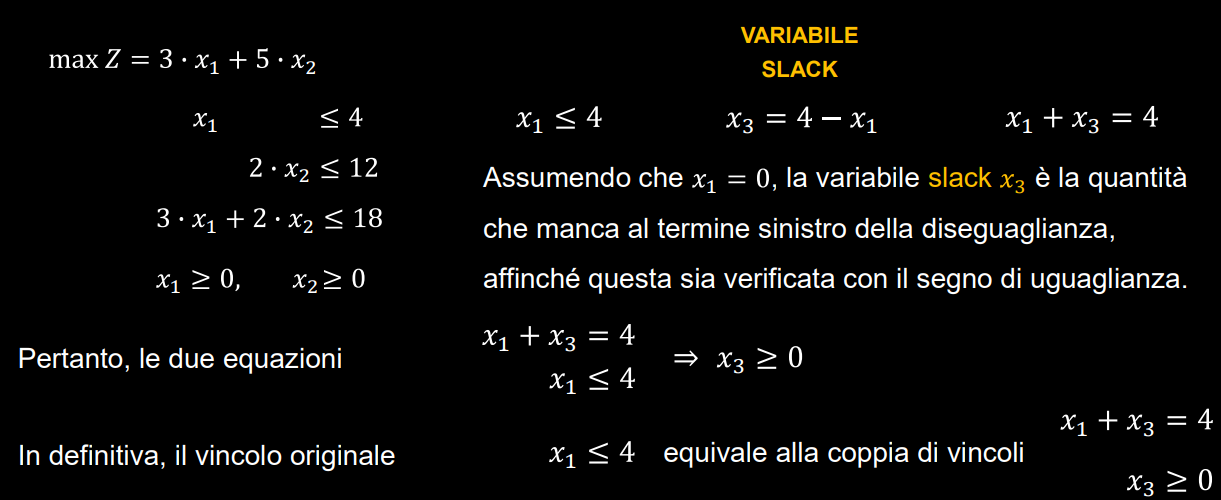
\includegraphics[width = 1\textwidth]{Images/20.PNG}
\end{center}
Introducendo una variabile slack per ognuno dei vincoli del problema di programmazione lineare in forma originale (\textbf{forma standard}) otteniamo una formulazione equivale detta:
\textbf{Modello in forma aumentata}:
\begin{center}
    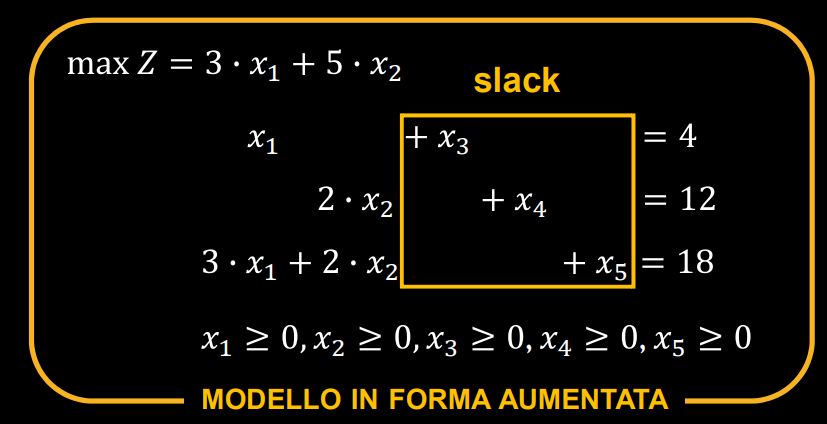
\includegraphics[width = 0.70\textwidth]{Images/21.PNG}
\end{center}
Se la \textbf{variabile slack di un vincolo assume valore zero}, allora la soluzione corrispondente giace sulla frontiera del vincolo della forma originale. (Il vincolo corrispondente della forma originale è verificato come uguaglianza). \newline
Se la \textbf{variabile slack di un vincolo assume valore positivo}, la soluzione corrispondente appartiene al semipiano ammissibile individuato dalla frontiera del vincolo della forma originale, vale a dire la soluzione appartiene alla regione ammissibile (è interna alla regione ammissibile). \newline
Se la \textbf{variabile slack di un vincolo assume valore negativo}, la soluzione corrispondente appartiene al semipiano non ammissibile della frontiera del vincolo della forma originale, vale a dire la soluzione non appartiene alla regione ammissibile. \newline
Si definisce \textbf{SOLUZIONE AUMENTATA}, una soluzione del modello in forma originale (valori della variabili decisionali) che viene "aumentata" tramite i corrispondenti valori delle variabili slack \newline
Si definisce \textbf{SOLUZIONE DI BASE} un vertice del modello in forma aumentata. Una soluzione di base può essere \textbf{ammissibile} o \textbf{non ammissibile}.
Si dice \textbf{SOLUZIONE DI BASE AMMISSIBILE} una soluzione associata a un \textbf{vertice ammissibile}, che venga aumentata.
\subsubsection{Variabili di base e non}
I termini \textbf{soluzione di base} e \textbf{soluzione di base ammissibile} sono molto importanti ed è quindi necessario chiarirne le \textbf{proprietà algebriche}:
per esempio, due variabili poste a 0 $x_1 = 0$ e $x_4 = 0$ vengono dette \textbf{variabili non di base}. Prendiamo il modello in forma aumentata sopra come esempio.
La \textbf{soluzione del sistema lineare} per le 3 variabili restanti, dette \textbf{variabili di base} $x_2 = 6, x_3 = 4, x_5 = 6$ porta alla seguente \textbf{soluzione di base}:
$$x_1 = 0, x_2 = 6, x_3 = 4, x_4 = 0, x_5 = 6$$
Il modello in forma aumentata consiste di 5 variabili (2 decisionali e 3 slack) e di 3 equazioni.
Abbiamo a disposizione quindi $2 = (5-3)$ \textbf{gradi di libertà} per risolvere il sistema lineare (il metodo del simplesso pone a zero il valore di due variabili, scelte arbitrariamente, per risolvere il sistema lineare). \newline
Le \textbf{proprietà algebriche} delle \textbf{SOLUZIONI DI BASE} e delle \textbf{SOLUZIONI DI BASE AMMISSIBILI} sono descritte tramite le seguenti definizioni: \newline
Una \textbf{SOLUZIONE DI BASE} gode delle seguenti proprietà:
\begin{enumerate}
    \item Una variabile può essere una \textbf{VARIABILE DI BASE} o una \textbf{VARIABILE NON DI BASE}
    \item IL numero delle variabili di base eguaglia il numero dei vincoli funzionali (equazioni). Pertanto, il numero delle variabili non di base eguaglia il numero totale delle variabili meno il numero dei vincoli funzionali
    \item Le variabili non di base vengono poste a zero
    \item I valori delle variabili di base sono ottenuti come una risoluzione simultanea del sistema di equazioni lineari (vincoli funzionali in forma aumentata). L'insieme delle variabili di base viene spesso riferito con il termine di \textbf{BASE}
    \item Se le variabili di base soddisfano i vincoli di non negatività, la \textbf{SOLUZIONE DI BASE} è una \textbf{SOLUZIONE AMMISSIBILE DI BASE}
\end{enumerate}
Così come certe coppie di vertici ammissibili sono tra loro adiacenti, le corrispondenti coppie di \textbf{soluzioni di base ammissibili} sono tra loro adiacenti: \newline
Due \textbf{SOLUZIONI DI BASE AMMISSIBILI} sono adiacenti se sono caratterizzate dal condividere le stesse \textbf{VARIABILI NON DI BASE} eccetto una. Questo implica che tutte le loro \textbf{VARIABILI DI BASE} sono uguali eccetto una, anche se esse possono assumere valori differenti.
Conseguentemente, muoversi dalla \textbf{SOLUZIONE DI BASE AMMISSIBILE} corrente ad una soluzione ad essa adiacente implica che una \textbf{VARIABILE NON DI BASE} divenga una \textbf{VARIABILE DI BASE} e che una \textbf{VARIABILE DI BASE} divenga una \textbf{VARIABILE NON DI BASE} (il che richiede di aggiustare i valori delle variabili di base per garantire che il sistema lineare di equazioni sia ancora soddisfatto).
Sempre considerando la regione ammissibile sopra, possiamo quindi notare che:
\begin{center}
    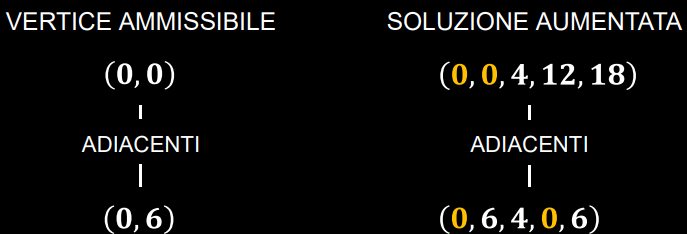
\includegraphics[width = 0.60\textwidth]{Images/22.png}
\end{center}
Quando si considera il problema in forma aumentata, è vantaggioso \textbf{considerare e manipolare la funzione obbiettivo} insieme ai vincoli.
Pertanto, prima di passare ad impiegare il metodo del simplesso, il problema deve essere riscritto in una forma equivalente che risulti adeguata.
Tenendo sempre come esempio il modello in forma aumentata presente sopra, esso quindi diventa:
\begin{center}
    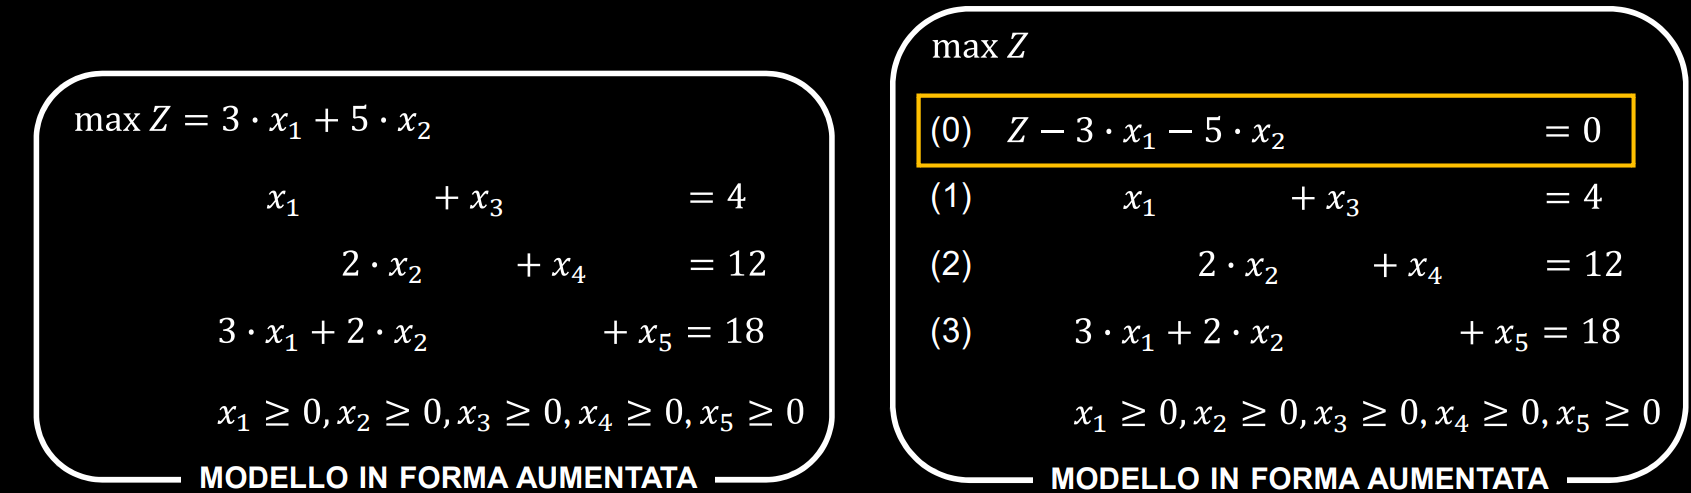
\includegraphics[width = 1\textwidth]{Images/23.png}
\end{center}
\subsubsection{Algoritmo del metodo del simplesso in forma algebrica}
Colleghiamo l'aspetto algebrico a quello geometrico per il metodo del simplesso.
L'\textbf{interpretazione geometrica} fa riferimento al \textbf{MODELLO IN FORMA STANDARD}. \newline
L'\textbf{interpretazione algebrica} fa riferimento al \textbf{MODELLO IN FORMA AUMENTATA}.
Presentiamo quindi l'algoritmo del metodo del simplesso in forma algebrica tenendo come esempio il modello presentato sopra:
\begin{enumerate}
    \item \textbf{INIZIALIZZAZIONE}: scegliere $x_1$ e $x_2$ come variabili non di base (perciò poste a valore nullo) per ottenere la soluzione iniziale di base ammissibile. Questo procedimento è giustificato dal \textbf{CONCETTO CHIAVE 3}
    \item \textbf{TEST DI OTTIMALITÀ}: $x_3, x_4$ e $x_5$ non compaiono nelle funzione obbiettivo $Z$, per cui sono i coefficienti delle variabili non di base, $x_1$ e $x_2$, a determinare il \textbf{TASSO DI CRESCITA} di $Z$.
    I \textbf{TASSI DI CRESCITA} sono rispettivamente 3 e 5, entrambi positivi, quindi la soluzione trovata sarà sicuramente \textbf{NON OTTIMALE}.
\end{enumerate}
Trattiamo inoltre come determinare la direzione di spostamento, assumendo di aver già trovato la soluzione di base iniziale:
\begin{enumerate}
    \item \textbf{DETERMINAZIONE DELLA DIREZIONE DI SPOSTAMENTO}: \newline aumentare il valore di una variabile non di base a partire da zero (modificano i valori delle variabili di base correnti per soddisfare le equazioni) equivale a spostarsi lungo uno degli spigoli che emanano dal corrente vertice ammissibile.
    La scelta di quale variabile non di base incrementare è effettuata in base al \textbf{CONCETTO CHIAVE 4} e al \textbf{CONCETTO CHIAVE 5}. Nel nostro esempio, aumenteremo $x_2$ poiché il suo tasso di miglioramento in $Z$ è 5, il quale è migliore del tasso di miglioramento in $Z$ dell'altra variabile non di base $x_1$.
    L'incremento del valore di questa variabile non di base, la fa divenire una variabile di base nella nuova soluzione di base; essa prende quindi il nome di \textbf{VARIABILE ENTRANTE}
    \item \textbf{DETERMINAZIONE DELL'INCREMENTO}: determina di quanto aumentare il valore della variabile entrante in base (nel nostro caso, $x_2$). Incrementare il valore di $x_2$ fa incrementare il valore della funzione obbiettivo $Z$, pertanto desideriamo aumentare il più possibile il valore di $x_2$ evitando però di abbandonare la regione ammissibile.
    Il soddisfacimento dei \textbf{vincoli} implica che se $x_2$ aumenta, mentre si mantiene il valore della variabile non di base $x_1$ uguale a zero, allora il valore di qualche altra variabile di base \textbf{deve variare}. L'ammissibilità richiede inoltre che \textbf{tutte le variabili siano non negative}. Le variabili non di base (inclusa quella entrante $x_2$) sono non negative, ma dobbiamo verificare quanto $x_2$ possa aumentare senza violare il vincolo di non negatività sulle variabili
    di base $x_3, x_4, x_5$. Per farlo, applichiamo il \textbf{TEST DEL RAPPORTO MINIMO}: prendiamo in considerazione tutti i vincoli a cui è soggetta la funzione obbiettivo e \textbf{ricaviamo da essi il massimo valore che possiamo assegnare a $x_2$ che non porti a violare i vincoli di non negatività sulle altre variabili}. Questo valore sarà quindi il più piccolo trovato:
    \begin{center}
        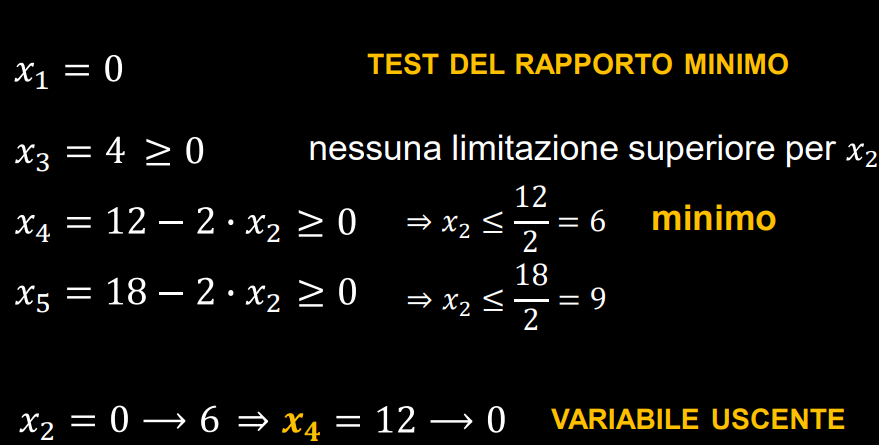
\includegraphics[width = 0.60\textwidth]{Images/24.png}
    \end{center}
    Questo passo dell'algoritmo va quindi a determinare quale variabile di base diminuisce a zero per prima quando si incrementa il valore della \textbf{VARIABILE ENTRANTE} in base.
    Diminuire il valore della variabile di base fino a raggiungere il valore zero trasforma questa variabile da variabile di base in variabile non di base nella nuova soluzione di base ammissibile.
    Pertanto, questa variabile è chiamata \textbf{VARIABILE USCENTE} dalla base all'iterazione corrente. 
    \item \textbf{DETERMINAZIONE DELLA NUOVA SOLUZIONE DI BASE}: Obbiettivo di questo passo è convertire il sistema lineare in una forma maggiormente vantaggiosa (forma adatta all'applicazione dell'\textbf{eliminazione Gaussiana}), al fine di applicare il test di ottimalità e (se necessario) di ottenere una nuova soluzione di base ammissibile.
    Nel nostro esempio, i valori di $x_3$ e $x_5$ nella nuova soluzione di base ammissibile vengono ottenuti come risultato di questo processo. Consideriamo di nuovo l'esempio
    Tenendo sempre come esempio il modello in forma aumentata presente sopra, esso quindi diventa:
    \begin{center}
        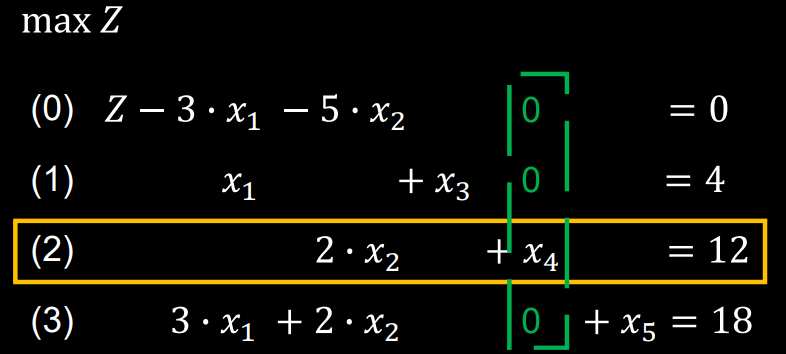
\includegraphics[width = 0.50\textwidth]{Images/25.png}
    \end{center}
    $x_2$ ha rimpiazzato $x_4$ come variabile di base nell'equazione (2). RIsolvere il sistema lineare rispetto a $Z, x_2, x_3, x_5$ richiede di applicare operazioni algebriche per \textbf{riprodurre il pattern $(0,0,1,0)$} di $x_4$ per $x_2$ (cioè fare in modo che il vettore colonna di $x_2$ diventi uguale al vettore colonna di $x_4$).
    Possiamo usare due tipi di operazioni algebriche:
    \begin{itemize}
        \item Moltiplicare (dividere) un'equazione per una costante non nulla
        \item Sommare (sottrarre) un multiplo di un'equazione per ottenere un'altra \newline equazione
    \end{itemize}
    \begin{center}
        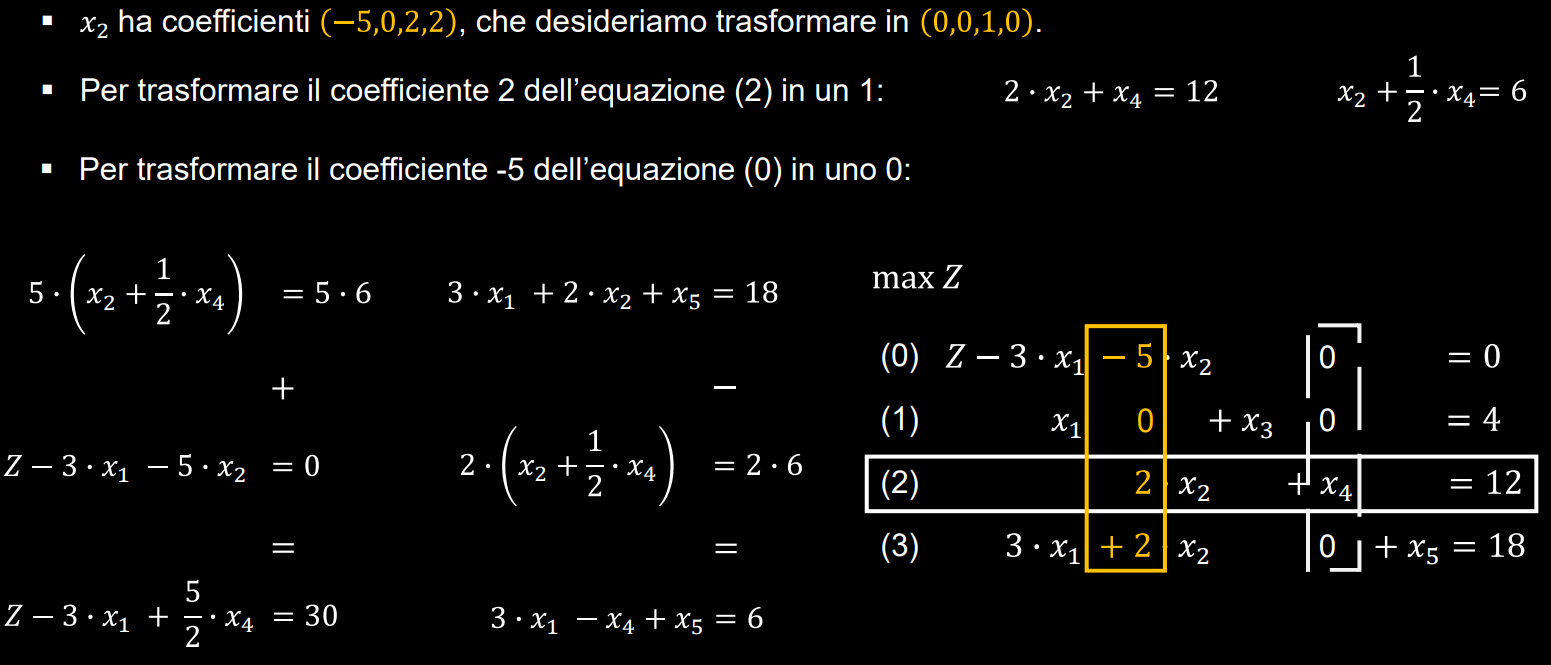
\includegraphics[width = 1\linewidth]{Images/26.png}
    \end{center}
    \begin{center}
        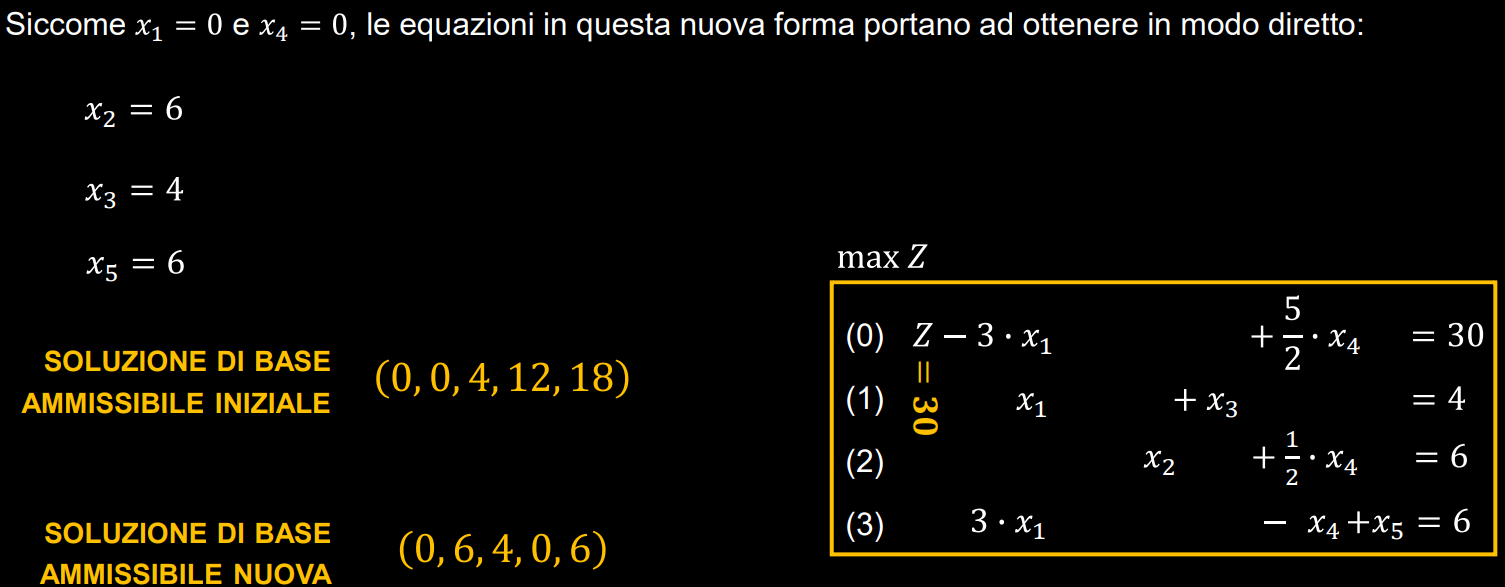
\includegraphics[width = 1\linewidth]{Images/27.png}
    \end{center}
    Questo processo è detto \textbf{eliminazione di Gauss-Jordan}: ogni variabile di base viene eliminata da tutte le equazioni tranne una dove ha coefficiente 1
\end{enumerate}
Applichiamo questo procedimento fino a quando i coefficienti della funzione obbiettivo \textbf{sono tutti negativi}, cioè abbiamo solo tassi di miglioramenti negativi.
La soluzione trovata in quel punto è la \textbf{soluzione ottimale}.
\subsection{Procedura tabellare per il metodo del simplesso}
La forma algebrica è la migliore per comprendere la logica sottostante il metodo del simplesso.
Comunque, la forma algebrica non è la più adeguata per effettuare le computazioni che abbiamo mostrato in precedenza, molto meglio in questo caso utilizzare la \textbf{forma tabellare} che
registra solo l'informazione essenziale:
\begin{itemize}
    \item Coefficienti delle variabili
    \item Termini noti delle equazioni
    \item Variabili di base per ogni equazione
\end{itemize}
La \textbf{forma tabellare} evita di memorizzare i simboli delle variabili in ogni equazione, ma cosa ancor più importante è rappresentata dal fatto che, è possibile evidenziare i numeri che sono coinvolti nelle computazioni ed è possibile memorizzare in modo
compatto tali numeri. La tabella da utilizzare ha la seguente struttura:
\begin{center}
    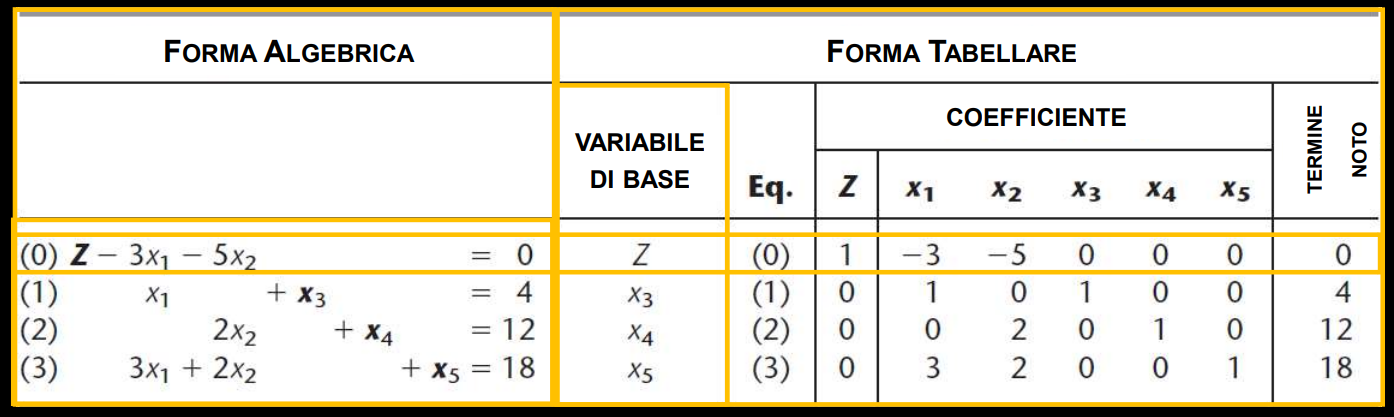
\includegraphics[width = 1\textwidth]{Images/28.PNG}
\end{center}
La tabella sopra è stata riempita \textbf{basandosi sull'esempio presentato fino ad ora}. Vediamo, sempre utilizzando questo esempio, tutti i passi del metodo del simplesso svolti con la forma tabellare:
\begin{itemize}
    \item \textbf{INIZIALIZZAZIONE}: Assumendo che il problema sia in forma standard, si procede come segue:
    \begin{itemize}
        \item Aggiungere le variabili slack
        \item Selezionare le variabili di decisione da porre a 0 (non di base)
        \item Selezionare le variabili slack come variabili di base
    \end{itemize}
    \begin{center}
        \vspace{-0.3cm}
        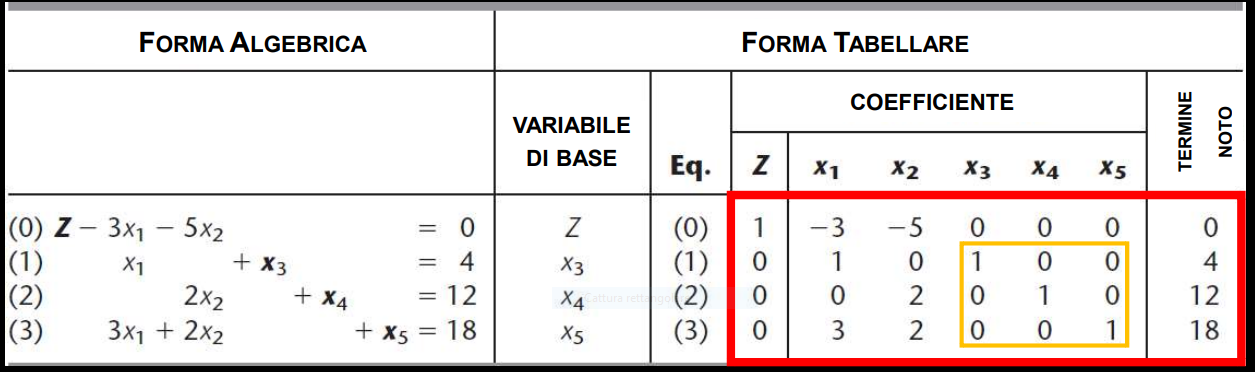
\includegraphics[width = 1\linewidth]{Images/29.PNG}
        \vspace{-1cm}
    \end{center}
    La parte della tabella che comprende le colonne dei valori di $Z, x_1, ..., x_5$ e dei termini noti viene detto \textbf{tableau}.
    Ricordiamo che, in questo caso, le variabili non di base sono $x_1$ e $x_2$ e che la soluzione di base ammissibile è $(0, 0, 4, 12, 8)$
    \item \textbf{TEST DI OTTIMALITÀ}: La \textbf{soluzione di base ammissibile corrente} è ottimale solo se tutti i \textbf{coefficienti della riga (0)} sono non negativi.
    Se questo è il caso, ci si arresta, altrimenti si effettua un'iterazione per ottenere una nuova soluzione di base ammissibile, il che implica che una variabile non di base venga trasformata in una variabile di base (passo 1)
    e viceversa (passo 2), per poi ottenere una nuova soluzione (passo 3).
    Vediamo i vari passi da effettuare in caso ci troviamo nella situazione in cui la soluzione non è ottimale:
    \begin{itemize}
        \item \textbf{ITERAZIONE: PASSO 1}: Identificare la \textbf{variabile entrante in base} (selezionandola tra quelle non di base) come quella cui corrisponde il \textbf{minimo coefficiente negativo nell'equazione (0)}.
        La colonna corrispondente viene denominata \textbf{colonna pivot}.
        \begin{center}
            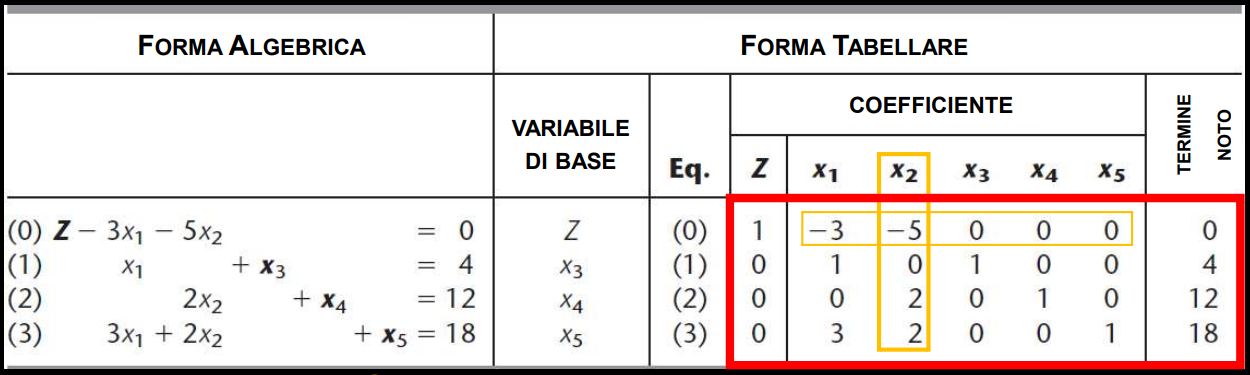
\includegraphics[width = 1\linewidth]{Images/30.PNG}
            \vspace{-0.7cm}
        \end{center}
        In questo caso, la variabile entrante sarà $x_2$.
        \item \textbf{ITERAZIONE: PASSO 2}: Determinate la \textbf{variabile di base uscente} tramite il \textbf{test del rapporto minimo}:
        \begin{enumerate}
            \item Selezionare i coefficienti strettamente positivi della colonna pivot
            \item Dividere i termini noti per questi coefficienti (riga omologa)
            \item Selezionare la riga cui corrisponde il più piccolo rapporto calcolato nel punto 2
            \item La variabile di quella riga è la variabile di base uscente, rimpiazzarla con la variabile entrante
        \end{enumerate}
        \begin{center}
            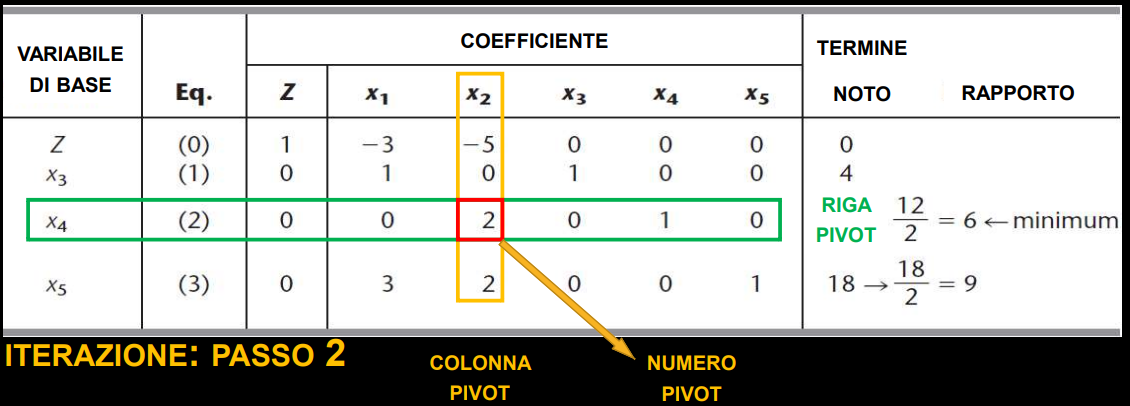
\includegraphics[width = 1\linewidth]{Images/31.PNG}
        \end{center}
        \item \textbf{ITERAZIONE: PASSO 3}: Determinare la nuova \textbf{soluzione di base} applicando operazioni che consentano l'uso dell'\textbf{eliminazione Gaussiana}.
        \begin{enumerate}
            \item Dividere la \textbf{riga pivot} per il \textbf{numero pivot}, ottenendo un nuovo \textbf{numero pivot} ed una nuova \textbf{riga pivot}
            \item Ad ogni altra riga (inclusa la riga 0) che abbia coefficiente negativo nella colonna pivot, sommare a questa riga il prodotto del valore assoluto del coefficiente per la nuova riga pivot
            \item Ad ogni altra riga (inclusa la riga 0) che abbia coefficiente positivo nella colonna pivot, sottrarre a questa riga il prodotto del valore assoluto del coefficiente per la nuova riga pivot
        \end{enumerate}
        \begin{center}
            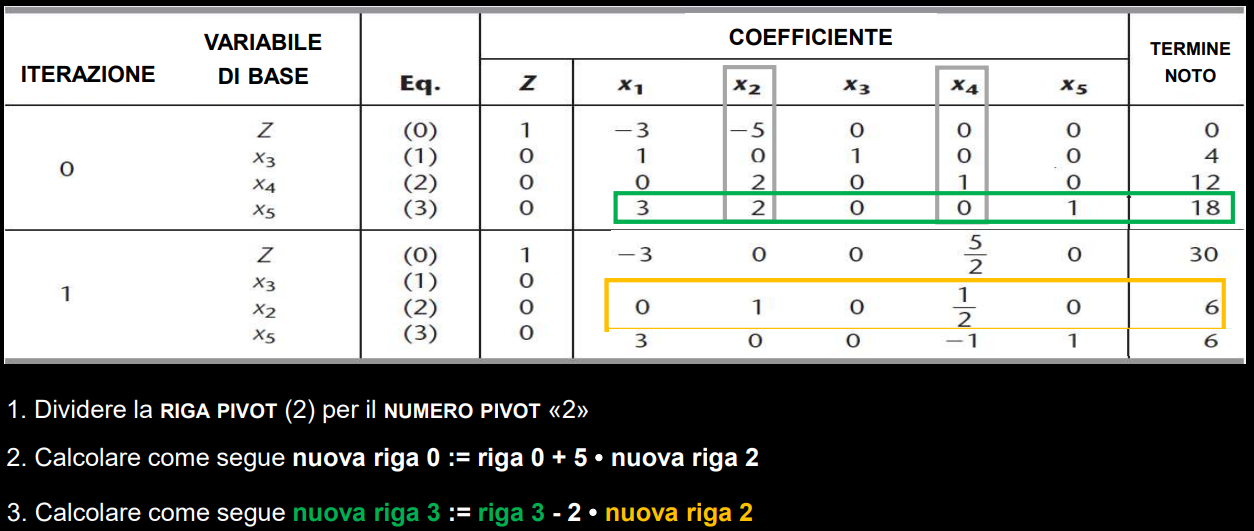
\includegraphics[width = 0.87\textwidth]{Images/32.PNG}
        \end{center}
        \item \textbf{TEST DI OTTIMALITÀ}: Controlliamo che la nuova riga 0 abbia tutti coefficienti non negativi; se è questo il caso ci fermiamo, altrimenti effettuiamo una nuova iterazione dell'algoritmo
    \end{itemize}
\end{itemize}
\newpage
\subsection{Tie Breaking}
Fino ad ora non abbiamo detto nulla in relazioni a situazioni nelle quali le regole adottate non portino a decisioni univoche, a causa di casi multipli o di ambiguità di vario genere.
I casi possibili, che tratteremo, sono i seguenti:
\begin{itemize}
    \item Alternative multiple per la variabile entrante in base
    \item Alternative multiple per la variabile uscente dalla base
    \item Mancanza di uan variabile uscente (funzione obbiettivo illimitata)
    \item Molteplici soluzioni ottimali
\end{itemize}
\subsubsection{Variabile entrante}
Il \textbf{passo 1} di ogni iterazione del \textbf{metodo del simplesso} sceglie come variabile entrante in base, la variabile non dib ase cui corrisponde il minimo valore (negativo) del coefficiente nell'equazione (0).
Supponiamo che due o più variabili non di base abbiano lo stesso valore minimo (negativo) per i rispettivi coefficienti dell'equazione (0). La scelta di quale variabile debba entrare in base può essere effettuata arbitrariamente.
La soluzione ottimale verrò comunque ottenuta, indipendentemente dalla variabile scelta come variabile entrante in base, e non sono disponibili metodi per prevedere quale scelta condurrà più rapidamente alla soluzione ottimale.
\subsubsection{Variabile uscente}
Supponiamo che al \textbf{passo 2 dell'algoritmo del simplesso} due o più variabili di base competano per uscire di base. \textbf{Fa differenza quale variabile viene scelta per uscire di base?}
\textbf{Assolutamente si}, è la fa in termini molto critici in base alla seguente catena di eventi:
\begin{itemize}
    \item Quando il valore della variabile di entrante viene aumentato, le variabili di base che sono selezionabili come variabili uscenti dalla base, raggiungono contemporaneamente il valore zero. Pertanto, le nuove variabili non selezionate come variabili uscenti avranno comunque
    un valore nullo nella nuova soluzione di base (una variabile di base che assume valore nullo è detta \textbf{variabile degenere})
    \item Se una \textbf{variabile degenere} mantiene il proprio valore nullo sino ad un'iterazione successiva, dove viene selezionata come variabile uscente, la corrispondente variabile entrante in base deve rimanere nulla (dato che non può essere aumentata senza far assumere un valore negativo alla variabile uscente).
    Pertanto il valore della funzione obbiettivo $Z$ resta invariato
    \item Se il valore della funzione obbiettivo $Z$ resta costante invece di aumentare ad ogni iterazione, il \textbf{metodo del simplesso potrebbe entrare in loop}, ripetendo la medesima sequenza di soluzioni senza raggiungere la soluzione ottimale. Sono stati prodotto esempi sintetici che mostrano come il metodo del simplesso venga
    \textbf{intrappolato in un loop perpetuo}. Tuttavia questo accade raramente e sono state sviluppate strategie apposite per controllare questa \textbf{situazione patologica}
\end{itemize}
\subsubsection{Nesuna variabile uscente}
Il \textbf{passo 2} di ogni iterazione del metodo del simplesso può portare ad un'ulteriore esito che non abbiano ancora discusso, vale a dire che nessuna variabile di base si qualifichi come variabile uscente di base (la stessa cosa non può accadere al \textbf{passo 1}, in quanto il test di ottimalità arresterebbe l'algoritmo).
Tale situazione si verifica se il valore della variabile entrante può essere aumentato illimitatamente senza implicare che il valore di almeno una variabile di base divenga negativo.
Nella \textbf{forma tabellare} significa che ogni coefficiente della \textbf{colonna pivot} (esclusa la riga 0) assume valore non positivo.
Il tableau quindi si può interpretare in questo modo: i vincoli non impediscono che il valore della funzione obbiettivo $Z$ cresca illimitatamente, pertanto il metodo del simplesso si arresta segnalando che il \textbf{valore della funzione obbiettivo $Z$ è illimitato}.
\subsubsection{Molteplici soluzioni ottimali}
Precedentemente, quando abbiamo introdotto il concetto di \textbf{SOLUZIONE OTTIMALE}, abbiamo precisato che \textbf{un problema di programmazione lineare può avere più di una soluzione ottimale}.
Quindi:
\begin{itemize}
    \item Ogni problema di PL che ammetta soluziono ottimali multiple (con regione ammissibile limitata) ha almeno \textbf{due vertici ammissibili} che sono \textbf{ottimali}
    \item Ogni soluzione ottimale è \textbf{combinazione convessa} di questi vertici ammissibili ottimali, cioè ogni soluzione è \textbf{esprimibile tramite una combinazione lineare del tipo}:
    $$\lambda_1 \boldsymbol{v_1} + \lambda_2 \boldsymbol{v_2}$$
    con $\boldsymbol{v_1}, \boldsymbol{v_2}$ i vertici ottimali e $\lambda_1 + \lambda_2 = 1$
    \item Di conseguenza, nella forma aumentata del problema di PL, \textbf{ogni soluzione ottimale risulta essere una combinazione convessa delle soluzioni di base ammissibili ottimali}.
\end{itemize}
Il metodo del simplesso si arresta automaticamente non appena individua una soluzione di base ottimale.
Comunque, in molte applicazioni di PL, sussistono fattori non tangibili, non inclusi nel modello di PL, sfruttabili per scegliere adeguatamente tra le soluzioni ottimali alternative. In questo caso, le soluzioni alternative devono essere comunque individuate.
Come menzionato, questo richiede di trovare tutte le altre soluzioni di base ottimali, e quindi ogni soluzione ottimale sarà calcolabile come combinazione convessa di tali soluzioni ottimali di base.
Una volta che il metodo del simplesso ha individuato una soluzione di base ottimale, è possibile identificare se ne esistono altre, ed in caso affermativo, trovarle come segue: se un problema ha più di una soluzione di base ottimale,
almeno \textbf{una delle variabili non di base ha un coefficiente nullo nella riga (0)}, il che implica che incrementare il valore di una qualsiasi di tali variabili \textbf{non cambia il valore della funzione obbiettivo $Z$}. Pertanto, queste altre
soluzioni di base ottimali sono identificabili (se necessario) effettuando ulteriori iterazioni del metodo del simplesso, scegliendo ogni volta una variabile non di base con coefficiente nullo come variabile entrante.
\subsection{Forme alternative}
Sino ad ora abbiamo presentato come applicare il metodo del simplesso assumendo che il problema di PL da risolvere fosse in \textbf{FORMA STANDARD}, cioè:
\begin{itemize}
    \item Problema di massimizzazione
    \item Vincoli di $\leq$
    \item Variabili di decisione non negative
\end{itemize}
Ora mostriamo come ricondurre un problema di PL in forma generica nel corrispondente problema in forma standard.
Tale trasformazione avverrà nella fase di inizializzazione, consentendo di applicare il metodo del simplesso esattamente come mostrato per la risoluzione della forma standard.
Consideriamo il seguente problema di programmazione lineare:
\begin{equation*}
    \begin{array}{ll}
        \displaystyle \textrm{min} & \; Z = -2 \cdot x_1 + 3 \cdot x_2\\
        \textrm{s.a.} & x_1 + x_2 = 7\\
        \phantom{} & x_1 - 2 \cdot x_2 \leq 4\\
        \phantom{} & x_1 \geq 0 \\
    \end{array}
\end{equation*}
Notiamo che:
\begin{itemize}
    \item È un problema di minimizzazione e non di massimizzazione
    \item C'è un vincolo di $=$
    \item Manca un vincolo di non negatività per $x_2$
\end{itemize}
Come facciamo a trasformarlo in un problema di PL in forma standard?
Per trasformare il problema di minimizzazione in un problema di massimizzazione, applichiamo la seguente formula:
$$\textrm{min} \; Z = -\textrm(max)\;(-Z)$$
Moltiplichiamo quindi la funzione obbiettivo per $-1$, ottenendo:
\begin{equation*}
    \begin{array}{ll}
        \displaystyle \textrm{max} & \; Z = 2 \cdot x_1 - 3 \cdot x_2\\
        \textrm{s.a.} & x_1 + x_2 = 7\\
        \phantom{} & x_1 - 2 \cdot x_2 \leq 4\\
        \phantom{} & x_1 \geq 0 \\
    \end{array}
\end{equation*}
Come facciamo a risolvere l'assenza del vincolo di \textbf{non negatività} per $x_2$?
Rimpiazziamo $x_2$ con \textbf{due variabili non negative} $x_2'$ e $x_2''$ con $x_2 = x_2' - x_2''$, ottenendo:
\begin{equation*}
    \begin{array}{ll}
        \displaystyle \textrm{max} & \; Z = 2 \cdot x_1 - 3 \cdot x_2' + 3\cdot x_2''\\
        \textrm{s.a.} & x_1 + x_2' - x_2''= 7\\
        \phantom{} & x_1 - 2 \cdot x_2' + 2 \cdot x_2'' \leq 4\\
        \phantom{} & x_1, x_2', x_2'' \geq 0 \\
    \end{array}
\end{equation*}
Come facciamo a trasformare un vincolo di $=$? Questo tipo di vincoli \textbf{possono essere sostituiti da due vincoli, uno di $\geq$ ed uno di $\leq$}.
Quindi otteniamo:
\begin{equation*}
    \begin{array}{ll}
        \displaystyle \textrm{max} & \; Z = 2 \cdot x_1 - 3 \cdot x_2' + 3\cdot x_2''\\
        \textrm{s.a.} & x_1 + x_2' - x_2'' \leq 7\\
        \phantom{} & x_1 + x_2' - x_2 '' \geq 7 \\
        \phantom{} & x_1 - 2 \cdot x_2' + 2 \cdot x_2'' \leq 4\\
        \phantom{} & x_1, x_2', x_2'' \geq 0 \\
    \end{array}
\end{equation*}
Moltiplichiamo per $-1$ il vincolo di $\geq$ e trasformiamolo in un vincolo di $\leq$:
\begin{equation*}
    \begin{array}{ll}
        \displaystyle \textrm{max} & \; Z = 2 \cdot x_1 - 3 \cdot x_2' + 3\cdot x_2''\\
        \textrm{s.a.} & x_1 + x_2' - x_2''\leq 7\\
        \phantom{} & -x_1 - x_2' + x_2 '' \leq 7 \\
        \phantom{} & x_1 - 2 \cdot x_2' + 2\cdot x_2'' \leq 4\\
        \phantom{} & x_1, x_2', x_2'' \geq 0 \\
    \end{array}
\end{equation*}
Infine, rinominiamo le variabili per \textbf{consistenza notazionale}, ottenendo:
\begin{equation*}
    \begin{array}{ll}
        \displaystyle \textrm{max} & \; Z = 2 \cdot x_1 - 3 \cdot x_2 + 3\cdot x_3\\
        \textrm{s.a.} & x_1 + x_2 - x_3 \leq 7\\
        \phantom{} & -x_1 - x_2 + x_3 \leq 7 \\
        \phantom{} & x_1 - 2 \cdot x_2 + 2 \cdot x_3 \leq 4\\
        \phantom{} & x_1, x_2, x_3 \geq 0 \\
    \end{array}
\end{equation*}
È sempre possibile convertire un problema di PL in forma standard. Tuttavia c'è da fare un osservazione:
quando moltiplichiamo un vincolo di $\geq$ per $-1$ per trasformarlo in un vincolo $\leq$, dobbiamo stare attenti
che il termine noto \textbf{non diventi negativo}; infatti il metodo del simplesso richiede che i termini noti siano
tutti non negativi. In questo caso, per evitare di effettuare passaggi in più, possiamo tenere il problema in forma non standard
e trasformarlo direttamente in forma aumentata, trasformando i vincoli nel seguente modo:
\begin{itemize}
    \item Per i vincoli di $\geq$ sottraiamo una \textbf{variabile di surplus}
    \item Per i vincoli di $\leq$ sommiamo una \textbf{variabile di slack}
\end{itemize}
\begin{center}
    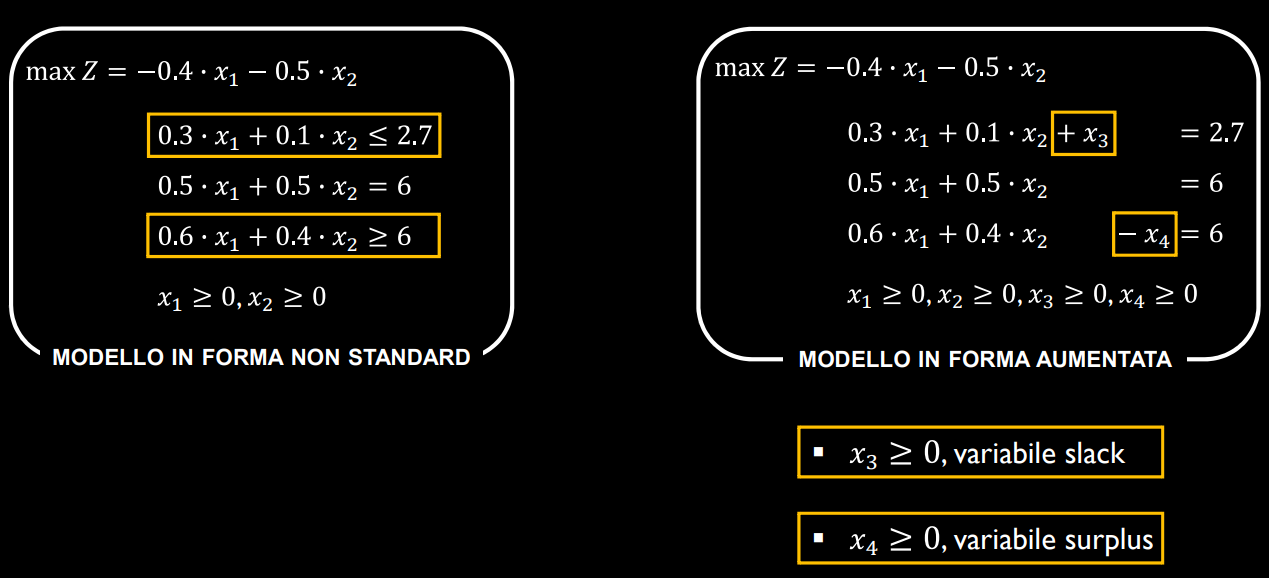
\includegraphics[width = 1\linewidth]{Images/34.PNG}
\end{center}
\subsection{Metodo delle 2 fasi}
Consideriamo un problema di programmazione lineare.
Ci possono essere dei casi dove la soluzione nulla \textbf{NON è una soluzione di base ammissibile per il problema considerato}: in particolare,
ciò si può notare dall'\textbf{assenza di una sottomatrice identità all'intendo della matrice dei coefficienti dei vincoli funzionali}.
Per applicare il metodo del simplesso dobbiamo quindi \textbf{calcolare una soluzione di base ammissibile iniziale}.
Per farlo usiamo la forma tabellare e applichiamo il \textbf{metodo delle 2 fasi}:
\begin{enumerate}
    \item \textbf{Aggiunta di variabili artificiali}: Aggiungiamo delle variabili artificiali in modo da ottenere una sottomatrice identità nella matrice dei
    coefficienti dei vincoli funzionali; questa sottomatrice identificherà i \textbf{termini da mettere in base}
    \item \textbf{Problema ausiliario (1° fase del simplesso)}: Il metodo delle due fasi prevede la risoluzione di un problema ausiliario che consiste nella minimizzazione
    della somma delle variabili artificiali introdotte; questo problema ausiliario mantiene i vincoli funzionali del problema originale. Risolviamo questo
    problema con il metodo del simplesso per trovare la soluzione di base ammissibile da cui partire per risolvere il problema originale. Possiamo ritrovarci nei seguenti casi:
    \begin{itemize}
        \item Il problema ausiliario ha \textbf{ottimo uguale a 0}:
        \begin{itemize}
            \item \textbf{Non ci sono variabili artificiali in base}: togliamo le colonne relative alle variabili artificiali e, tenendo i valori ottenuti nell'ultimo tableau del problema ausiliario,
            riportiamo la funzione obbiettivo originale nella riga 0 del tableau. Risolviamo quindi il tableau ottenuto applicando il metodo del simplesso
            \item \textbf{Ci sono variabili artificiali in base}: Si devono portare fuori dalla base, poi si procede come sopra
        \end{itemize}
        \item Il problema ausiliario ha \textbf{ottimo diverso da 0}: Il problema originale non ha soluzioni
    \end{itemize}
\end{enumerate}
\subsection{Teoria del simplesso}
Fino ad ora abbiamo utilizzato un esempio specifico per introdurre il concetto di \textbf{vertice ammissibile} e per chiarire il ruolo che gioca
nel \textbf{metodo del simplesso}. Nello specifico, abbiamo fornito un'interpretazione geometrica e una corrispondente interpretazione algebrica del metodo del simplesso.
Come facciamo tuttavia a \textbf{generalizzare} questi concetti nel caso di problemi di programmazione lineare con un maggior numero di variabili decisionali e con un maggior numero di vincoli?
È intuitivo pensare che le \textbf{soluzioni ottimali} di un problema di programmazione lineare giacciano \textbf{sulla frontiera della regione ammissibile}, ed infatti ciò corrisponde al vero.
A causa del fatto che la frontiera è un concetto geometrico, la prima definizione che forniamo mira a chiarire come identificare algebricamente la frontiera per una data regione ammissibile.
\textbf{L'equazione della frontiera di un vincolo viene ricavata con le seguenti sostituzioni}:
\begin{itemize}
    \item $\leq \rightarrow =$
    \item $\geq \rightarrow =$ 
\end{itemize}
\textbf{L'equazione della frontiera di un vincolo funzionale è}:
$$a_{i1} \cdot x_1 + a_{i2} \cdot x_2 + ... + a_{in} \cdot x_n = b_i$$
mentre per un \textbf{vincolo di non negatività} abbiamo $x_j = 0$.
Ogni equazione definisce una \textbf{figura geometrica "piatta"}, che prende il nome di \textbf{IPERPIANO} nello spazio \textbf{n-dimensionale}, l'analogo di una retta nello spazio
2-dimensionale e di un piano nello spazio 3-dimensionale.
\begin{itemize}
    \item Quando il vincolo è di $\leq$ o di $\geq$, l'iperpiano separa i punti che verificano il vincolo da quelli che lo violano
    \item Quando il vincolo è di $=$, solo i punti che giacciono sull'iperpiano verificano il vincolo
\end{itemize}
La \textbf{frontiera della regione ammissibile} contiene solo quelle soluzioni ammissibili che soddisfano una o più equazioni di frontiera.
Geometricamente, \textbf{ogni punto sulla frontiera della regione ammissibile giace su uno o più iperpiani definiti dalle rispettive equazioni di frontiera}.
\begin{center}
    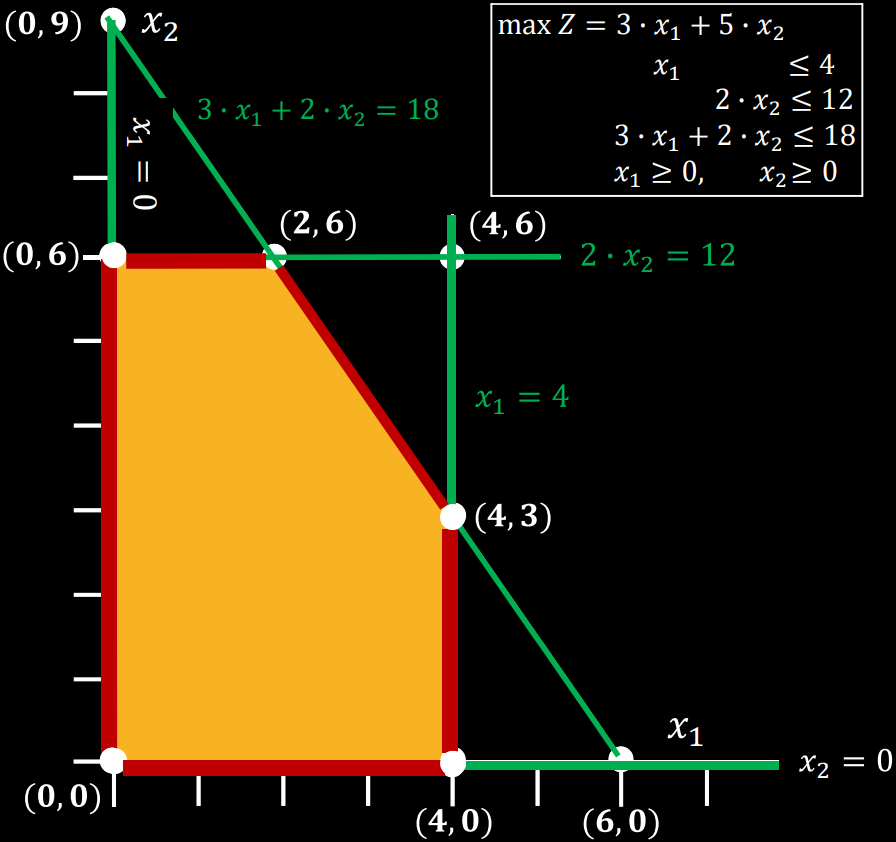
\includegraphics[width = 0.60\linewidth]{Images/35.png}
\end{center}
Un \textbf{vertice ammissibile} è una soluzione ammissibile che non giace su un segmento che connette altre due soluzioni ammissibili.
Una soluzione che giace su un segmento che collega due altre soluzioni ammissibili \textbf{non è un vertice ammissibile}. prendendo l'esempio sopra quindi:
\begin{itemize}
    \item $(2,3)$ \textbf{non è un vertice ammissibile}, giace sul segmento che collega $(0,3)$ e $(4,3)$
    \item $(0,3)$ \textbf{non è un vertice ammissibile}, giace sul segmento che collega $(0,0)$ e $(0,6)$
    \item $(0,0)$ \textbf{è un vertice ammissibile}, non esistono due soluzioni ammissibili tali per cui $(0,0)$ giaccia sul segmento che collega tra loro tali soluzioni ammissibili
\end{itemize}
Se il numero di variabili di decisione è 2 o 3, la definizione di vertice ammissibile che abbiamo appena fornito non è particolarmente efficace per identificare tali soluzioni.
Pertanto, si dimostrerà più utile interpretare queste soluzioni in termini algebrici. In ogni problema di programmazione lineare con 2 ($n = 2$) variabili di decisione, ogni vertice ammissibile giace all'intersezione
di 2 ($n = 2$) vincoli, vale a dire che ogni vertice ammissibile è la soluzione di un sistema lineare di 2 equazioni di frontiera.
In ogni problema di programmazione lineare con $n$ variabili di decisione, \textbf{ogni vertice ammissibile giace all'intersezione di $n$ frontiere di altrettanti vincoli}, vale a dire ogni vertice è la soluzione simultanea
di un sistema di \textbf{$n equazioni$}, ognuna rappresentante la frontiera di uno degli $n$ vincoli.
Comunque, \textbf{questo non significa che ogni insieme di $n$ equazioni di frontiera, comunque scelte tra gli $n+m$ vincoli} ($n$ vincoli di non negatività ed $m$ vincoli funzionali), \textbf{determini un vertice ammissibile}.
In particolare, la soluzione simultanea di un tale sistema lineare potrebbe violare uno più degli $m$ vincoli che non sono stati selezionati per definire il sistema lineare, nel qual caso il vertice individuato sarebbe un \textbf{VERTICE NON AMMISSIBILE}.
Inoltre, \textbf{un sistema di $n$ equazioni potrebbe non ammettere soluzioni}, tuttavia sistemi di questo tipo non sono di interesse.
Ultima possibilità è che \textbf{esistano soluzioni multiple dovute a equazioni ridondanti}. Il simplesso gestisce per noi queste situazioni.
È anche possibile che \textbf{più di un sistema costituito da $n$ equazioni abbia il medesimo vertice come soluzione}.
\subsubsection{Vertici ammissibili adiacenti}
Precedentemente abbiamo detto che, quando si ignorano le \textbf{variabili di slack e di surplus}, ogni iterazione dell'algoritmo del simplesso equivale allo spostamento dal corrente vertice ammissibile a un vertice ammissibile a lui adiacente.
È normale quindi porsi le seguenti domande:
\begin{itemize}
    \item Che \textbf{cammino} segue il metodo del simplesso?
    \item Cosa è un \textbf{vertice ammissibile adiacente}?
\end{itemize}
Partiamo con l'affrontare queste domande dal punto di vista geometrico:
consideriamo il seguente esempio con 2 variabili decisionali:
\begin{center}
    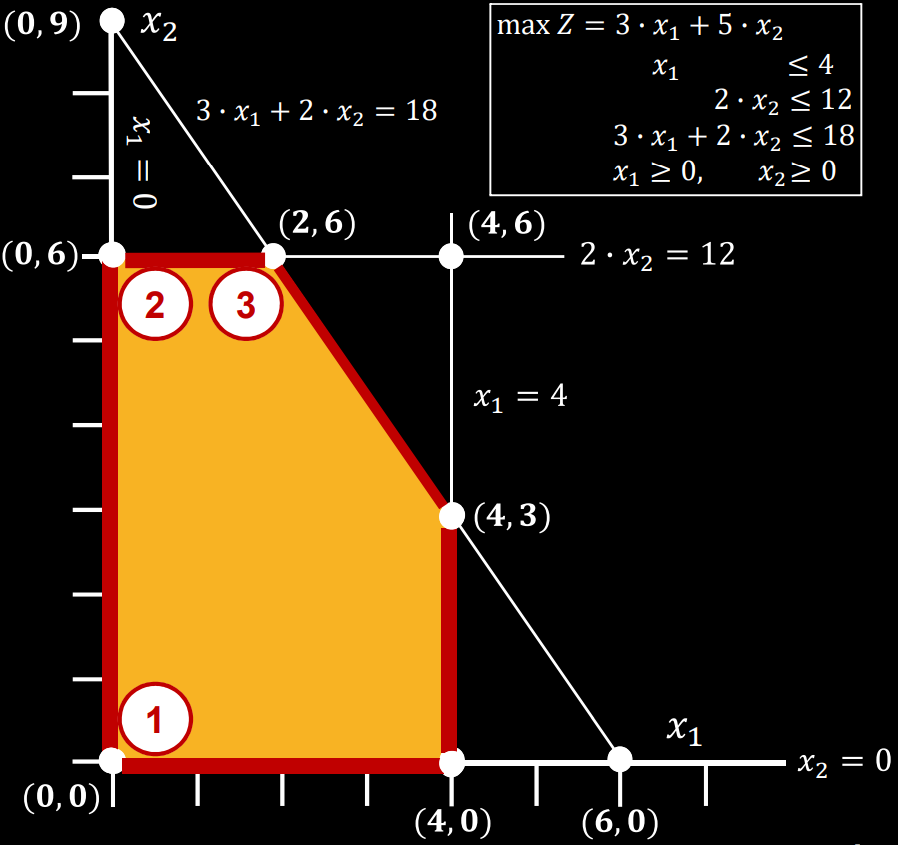
\includegraphics[width = 0.50\linewidth]{Images/36.png}
\end{center}
la frontiera della regione ammissibile è determinata dai sui \textbf{spigoli}.
Da ogni vertice ammissibile emanano due spigoli che conducono ai vertici a lui adiacenti.
Il cammino seguito dal metodo del simplesso, nel caso in cui si parta dal vertice ammissibile (0,0), è mostrato nella
figura ($1 \rightarrow 2 \rightarrow 3$). Ogni movimento porta ad un vertice ammissibile adiacente, implicando un \textbf{solo cambio nel sistema di equazioni}
\begin{center}
    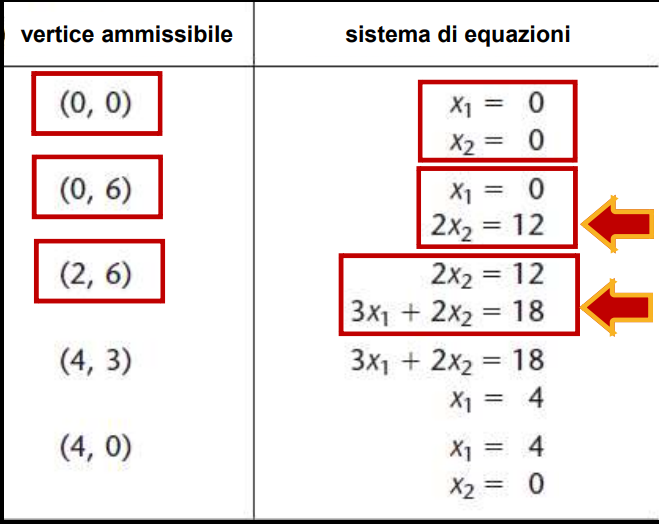
\includegraphics[width = 0.50\linewidth]{Images/37.png}
\end{center}
Nel caso in cui $n = 3$, le cose diventano un poco più complesse. Consideriamo il seguente esempio:
\begin{center}
    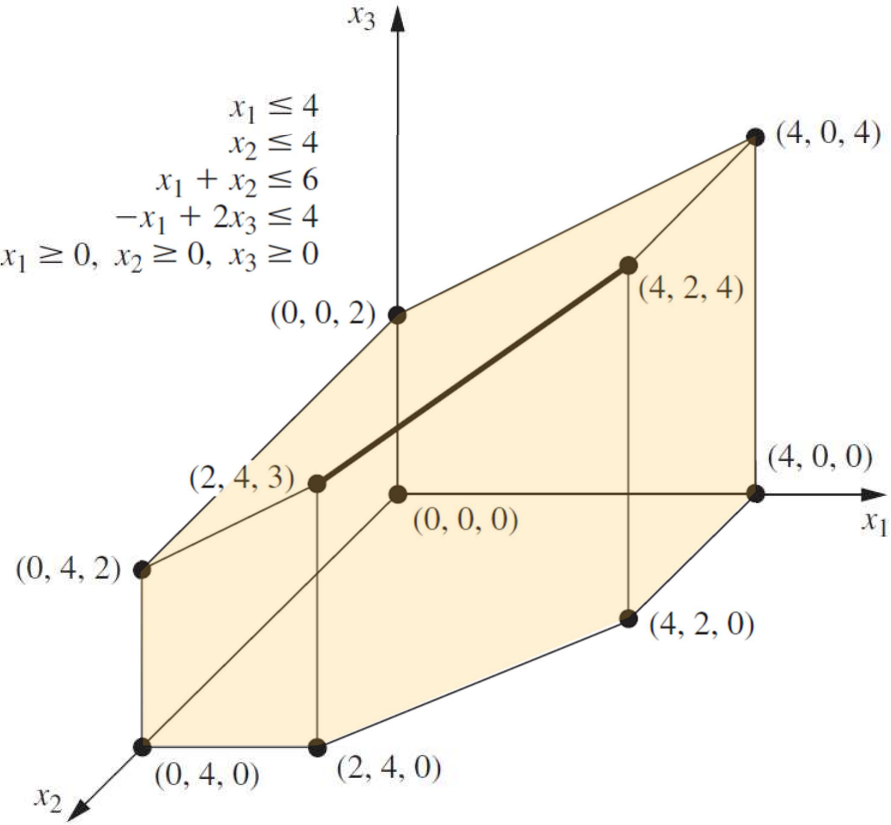
\includegraphics[width = 0.60\linewidth]{Images/38.png}
\end{center}
Come possiamo notare:
\begin{itemize}
    \item La \textbf{regione ammissibile} non è più un poligono come nel caso $n = 2$ ma è invece un \textbf{poliedro}
    \item Le \textbf{equazioni di frontiera} sono \textbf{piani} e non più \textbf{rette} come nel caso $n = 2$
    \item Ogni vertice ammissibile giace all'intersezione di 3 equazioni di frontiera, verificando anche i vincoli restanti
    \item Le intersezioni che non soddisfano uno o più dei restanti vincoli individuano \textbf{vertici non ammissibili}
\end{itemize}
\begin{center}
    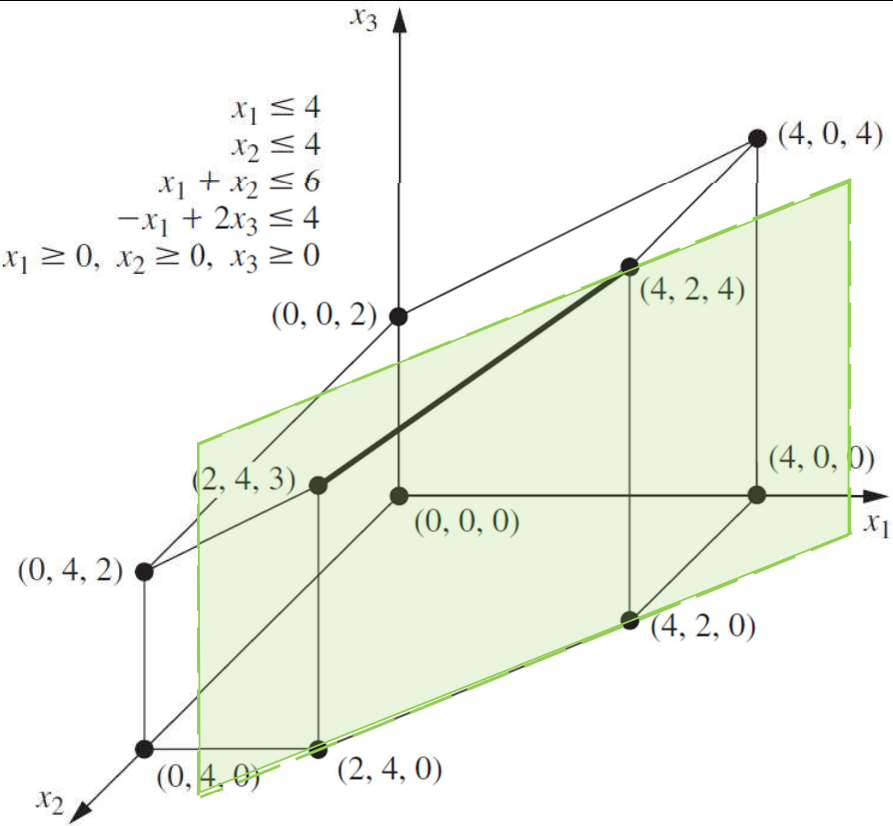
\includegraphics[width = 0.60\linewidth]{Images/39.png}
\end{center}
Facciamo un esempio di \textbf{cammino del metodo del simplesso}: supponiamo di partire dal vertice $(2, 4, 3)$ e che l'algoritmo
ci porti a spostarsi nel vertice $(4, 2, 4)$.
\begin{center}
    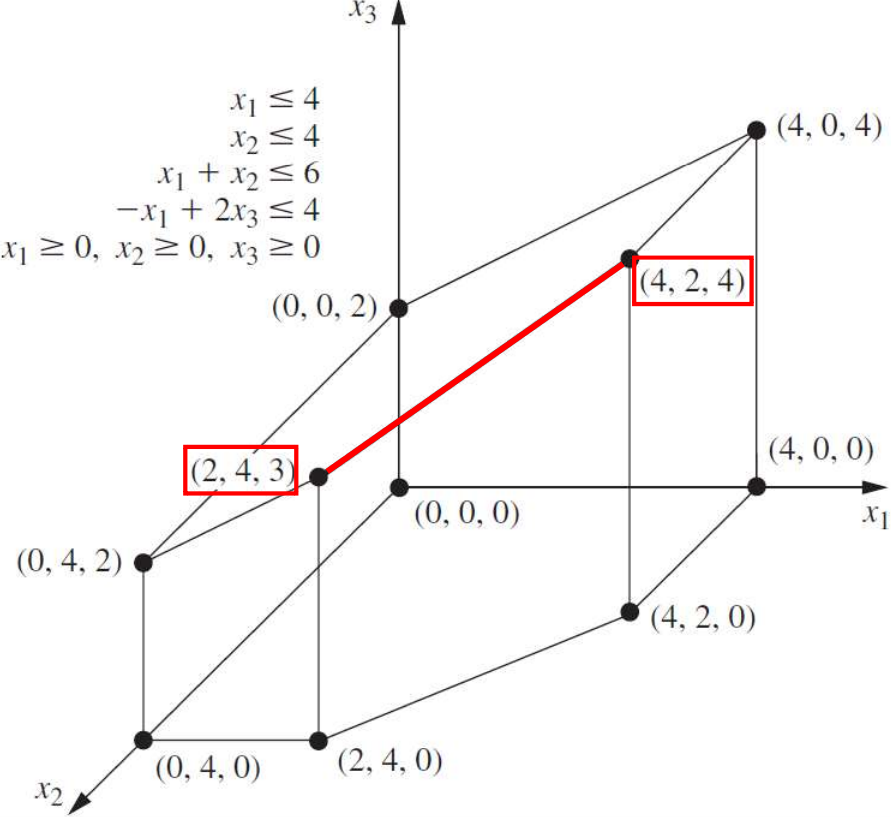
\includegraphics[width = 0.60\linewidth]{Images/40.png}
\end{center}
\noindent Il vertice $(2, 4, 3)$ giace all'intersezione delle seguenti equazioni di frontiera:
\begin{equation*}
    \begin{cases}
        x_2 = 4 \\
        x_1 + x_2 = 6 \\
        -x_1 + 2 \cdot_x3 = 4
    \end{cases}
\end{equation*}
\begin{center}
    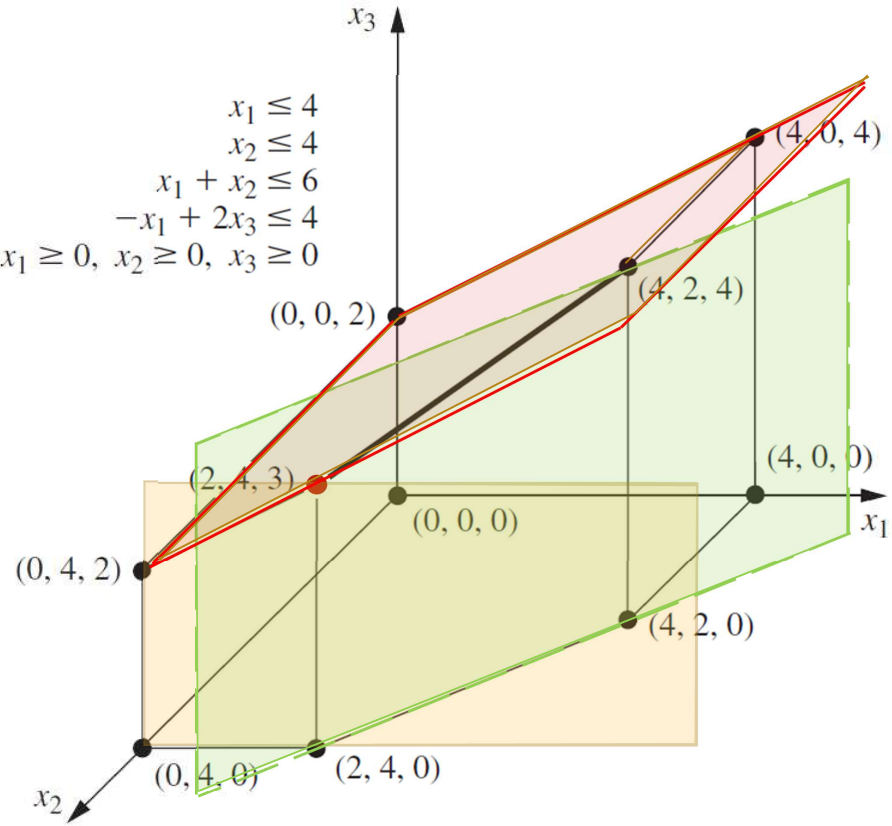
\includegraphics[width = 0.60\linewidth]{Images/41.png}
\end{center}
\noindent I $(2, 4, 3)$ e $(4, 2, 4)$ sono \textbf{vertici adiacenti}. Per $n=3$ tutti gli \textbf{spigoli della regione ammissibile} sono formati analogamente,
come intersezione di coppie di equazioni di frontiera.
\begin{center}
    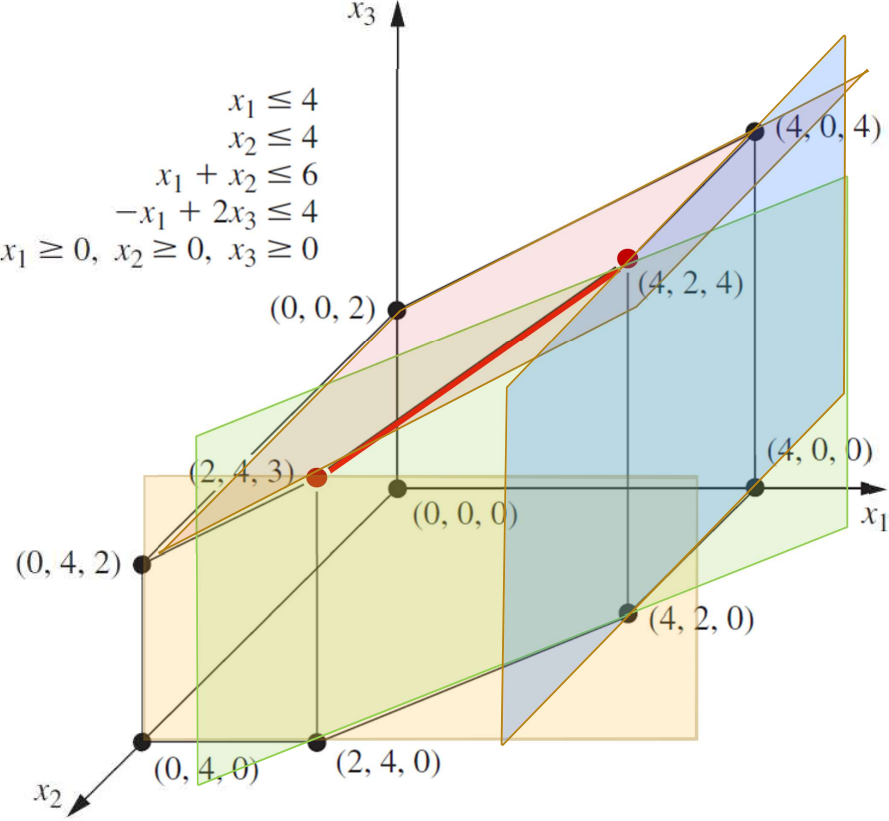
\includegraphics[width = 0.60\linewidth]{Images/42.png}
\end{center}
Per il vertice ammissibile $(2, 4, 3)$ abbiamo tre modi di rimuovere un'equazione delle tre sopra riportate.
Ogni modo porta ad un vertice adiacente differente
\begin{center}
    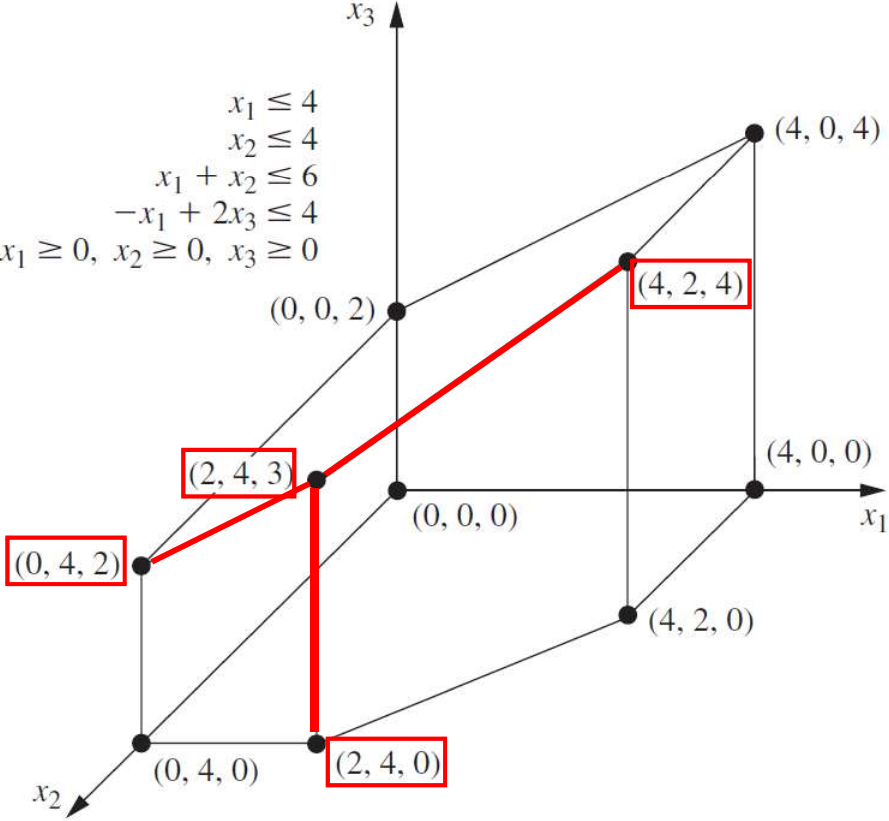
\includegraphics[width = 0.60\linewidth]{Images/43.png}
\end{center}
Se $n>3$, i concetti esposti generalizzano, eccezion fatta per le frontiere dei vincoli che ora sono \textbf{iperpiani} al posto di \textbf{piani} come nel caso $n = 3$.
Dato un problema di programmazione lineare con $n$ \textbf{variabili decisionali e regione ammissibile limitata} avremo che:
\begin{itemize}
    \item \textbf{Un vertice ammissibile giace all'intersezione di $n$ equazioni di frontiera} (e soddisfa anche i restanti vincoli)
    \item \textbf{Uno spigolo della regione ammissibile è un segmento che giace all'intersezione di $n-1$ equazioni di frontiera}, dove ogni vertice stremo giace su un'equazione di frontiera addizionale (tale che gli estremi siano vertici ammissibili)
    \item \textbf{Due vertici ammissibili sono adiacenti se il segmento che li collega è uno spigolo della regione ammissibile}
    \item \textbf{Da ogni vertice ammissibile emanano $n$ spigoli, ognuno conduce ad uno degli $n$ vertici ammissibili adiacenti}
    \item \textbf{Ogni iterazione del metodo del simplesso si sposta dal corrente vertice ammissibile ad un vertice ammissibile adiacente muovendosi su questi spigoli}
\end{itemize}
Passando all'interpretazione \textbf{algebrica} avremo che \textbf{l'intersezione delle equazioni di frontiera equivale alla loro risoluzione simultanea in termini del corrispondente sistema lineare}.
Alcune implicazioni di quanto abbiamo appena presentato sono:
\begin{itemize}
    \item Quando il metodo del simplesso \textbf{sceglie la variabile entrante in base}, l'interpretazione geometrica è che il metodo del simplesso stia \textbf{scegliendo uno degli spigoli che emanano dal vertice ammissibile corrente}
    \item \textbf{Aumentare il valore della variabile entrante in base}, a partire dal valore zero, e contemporaneamente variare il valore delle restanti variabili di base, \textbf{corrisponde a muoversi lungo lo spigolo scelto}
    \item Il valore di una delle variabili di base correnti, in particolare la \textbf{variabile uscente dalla base}, viene ridotto fino a raggiungere il valore zero, il che significa che il \textbf{raggiungimento della frontiera del vincolo} che si trova all'altro \textbf{estremo dello spigolo} della regione ammissibile
\end{itemize}
\subsubsection{Proprietà dei vertici ammissibili}
In un problema di programmazione lineare che abbia soluzioni ammissibili e con regione ammissibile limitata, i vertici ammissibili hanno le seguenti proprietà:
\begin{itemize}
    \item \textbf{PROPRIETÀ 1}:
    \begin{itemize}
        \item Se esiste solo una soluzione ottimale, allora questa è un \textbf{vertice ammissibile}. In ogni problema che ammette una sola soluzione ottimale, è sempre possibile far aumentare il valore della funzione obbiettivo fino a che non si raggiunga un vertice (la soluzione ottimale) della regione ammissibile.
        \item Se esistono soluzioni ottime multiple (e la regione ammissibile è limitata), allora \textbf{almeno due di queste soluzioni sono vertici ammissibili tra loro adiacenti}. Nel caso di $n = 2$, la risoluzione grafica consisterebbe nel far aumentare la funzione obbiettivo sino a farla sovrapporre con il segmento (spigolo) che connette due vertici ammissibili.
        Lo stesso accadrebbe nel caso di più variabili di decisione, tranne che in questo caso la funzione obbiettivo sarebbe associata ad un iperpiano che verrebbe fatto aumentare sino a toccare lo(gli) spigolo(i) tali da collegare vertici ammissibili adiacenti. Come conseguenza, \textbf{tutte le soluzioni ottimali sono ottenibili come media pesata dei vertici ammissibili ottimali}
    \end{itemize}
    \item \textbf{PROPRIETÀ 2}: Ogni vertice ammissibile è soluzione di un sistema lineare formato da $n$ equazioni scelte tra $m+n$ vincoli ($n$ vincoli di non negatività ed $m$ vincoli funzionali).
    Il numero di combinazioni di $m+n$ vincoli, presi a gruppi di $n$, è pari a:
    $$\binom{m+n}{n} = \frac{(m+n)!}{m!n!}$$
    che è un numero finito. Questa quantità rappresenta un \textbf{limite superiore al numero di vertici ammissibili}.
    \item \textbf{PROPRIETÀ 3}: Se un vertice ammissibile non ha vertici ammissibili a lui adiacenti che coincidono con soluzioni con valore migliore della funzione obbiettivo $Z$, allora non esistono soluzioni ottimali migliori di quella che coincide con il vertice ammissibile in esame.
    Pertanto, un tal vertice, in base alla \textbf{PROPRIETÀ 1}, è garantito coincidere con una soluzione ottimale, e questo semplicemente assumendo che il problema di PL considerato ammetta almeno una soluzione ottimale, il che è garantito se si assume che il problema di PL abbia soluzione ammissibile e la sua regione ammissibile sia limitata.
    La motivazione base per la quale questa proprietà è sempre valida in un problema di PL è che \textbf{la regione ammissibile è sempre un INSIEME CONVESSO}:
    \begin{itemize}
        \item Un \textbf{insieme} viene detto \textbf{convesso} se è una collezione di punti tali che, per ogni coppia di punti appartenenti alla collezione, l'intero segmento che collega la coppia di punti appartiene anch'esso alla collezione.
    \end{itemize}
    Nel caso di un problema di PL con due variabili decisionali, la \textbf{proprietà di convessità} significa che l'angolo interno alla regione ammissibile misurato in ogni vertice ammissibile è \textbf{minore di 180°}.
\end{itemize}
\subsection{Teoria della dualità}
Uno degli sviluppi più importanti della programmazione lineare è il concetto di \textbf{dualità} insieme alle sue importanti ramificazioni.
Questi sviluppi hanno rivelato che ogni problema di programmazione lineare ha associato un'altro problema di programmazione lineare chiamato \textbf{DUALE}.
Le relazioni esistenti tra il \textbf{PROBLEMA DUALE} ed il problema originale, chiamato \textbf{PROBLEMA PRIMALE}, si dimostrano utili da diversi punti di vista.
Per esempio, mostreremo in seguito che i \textbf{prezzi ombra} sono forniti dalla \textbf{soluzione ottimale del problema duale}.
Uno degli utilizzi più importanti della teoria della dualità è relativo a interpretazione e implementazione dell'\textbf{analisi di sensitività}.
L'analisi si sensitività è una componente molto importante in ogni studio che coinvolga un modello di programmazione lineare.
Infatti, molti dei parametri utilizzati nel modello originale non sono altro che stime di condizioni che si realizzeranno in condizioni future, e pertanto è necessario studiare quale sia l'effetto
sulla soluzione ottimale nel caso in cui alla prova dei fatti si realizzino condizioni differenti da quelle ipotizzate.
Inoltre, i valori di alcuni parametri (come ad esempio le quantità di risorse rese disponibili) dipendono da decisioni manageriali, in questo caso la scelta del valore dei parametri può rappresentare la questione principale da investigare tramite l'analisi della sensitività.
Vediamo quindi quali sono le relazioni tra problema primale e problema duale:
\begin{center}
    \noindent
    \makebox[\textwidth]{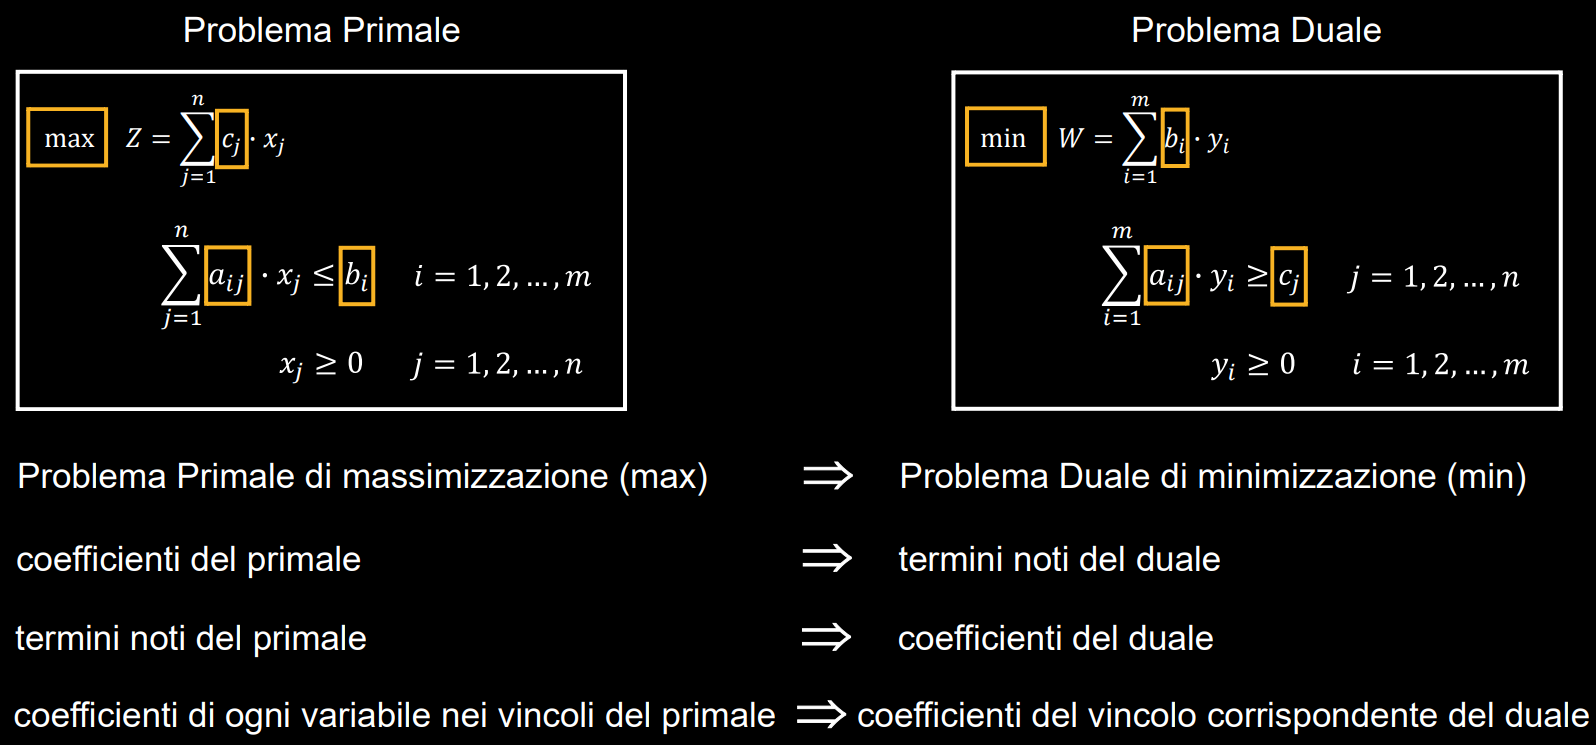
\includegraphics[width = 0.80\paperwidth]{Images/44.png}}
\end{center}
Per enfatizzare il parallelismo tra Primale e Duale, procediamo in forma matriciale:
il problema primale si può descrivere nel seguente modo:
\begin{equation*}
    \begin{array}{ll}
        \displaystyle \textrm{max} & \; Z = \boldsymbol{c}\boldsymbol{x}\\
        \textrm{s.a.} & \boldsymbol{A}\boldsymbol{x} \leq \boldsymbol{b}\\
        \phantom{} & \boldsymbol{x} \geq 0 \\
    \end{array}
\end{equation*}
Con $\boldsymbol{c} = [c_1, c_2, ..., c_n]$, $\boldsymbol{x} = \begin{bmatrix}
    x_1 \\
    x_2 \\
    \vdots \\
    x_n
\end{bmatrix}$ e $A = [a_{ij}]$ è la matrice $m \times n$ dei coefficienti tecnologici.
Il problema duale corrispondente può essere quindi descritto nel seguente modo:
\begin{equation*}
    \begin{array}{ll}
        \displaystyle \textrm{min} & \; W = \boldsymbol{y}\boldsymbol{b}\\
        \textrm{s.a.} & \boldsymbol{y}\boldsymbol{A} \geq \boldsymbol{c}\\
        \phantom{} & \boldsymbol{y} \geq 0 \\
    \end{array}
\end{equation*}
con $y = [y_1, y_2, ..., y_m]$ e $\boldsymbol{b} = \begin{bmatrix}
    b_1 \\
    b_2 \\
    \vdots \\
    b_m
\end{bmatrix}$. \newline
Facciamo un esempio:
\begin{center}
    \vspace{-0.2cm}
    \makebox[\textwidth]{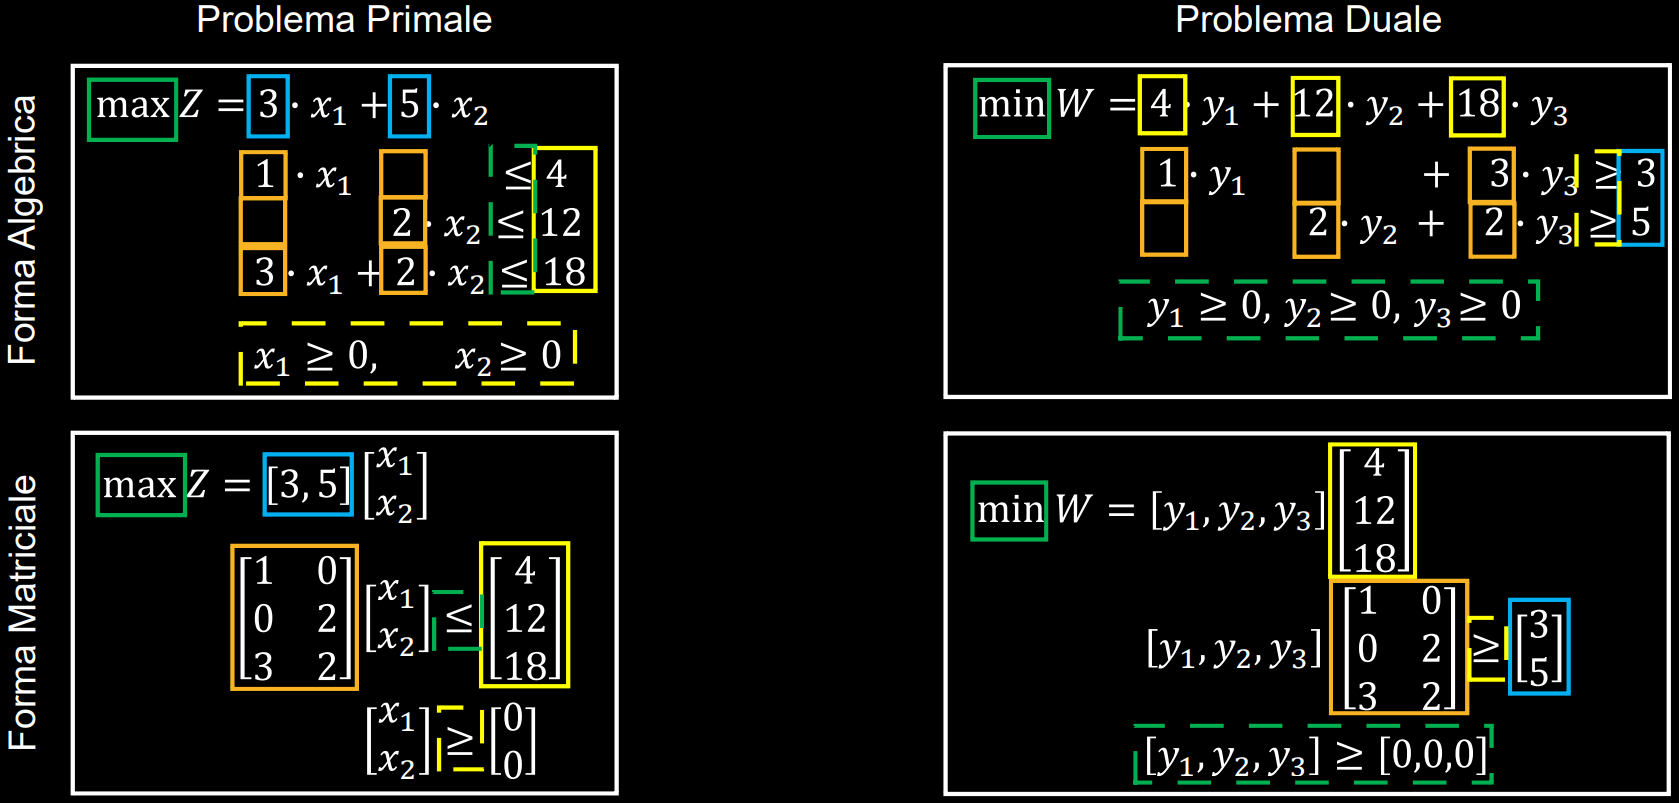
\includegraphics[width = 0.90\paperwidth]{Images/45.png}}
\end{center}
\newpage \noindent
La relazione tra primale e duale si può tradurre anche in \textbf{forma tabellare}:
\begin{center}
    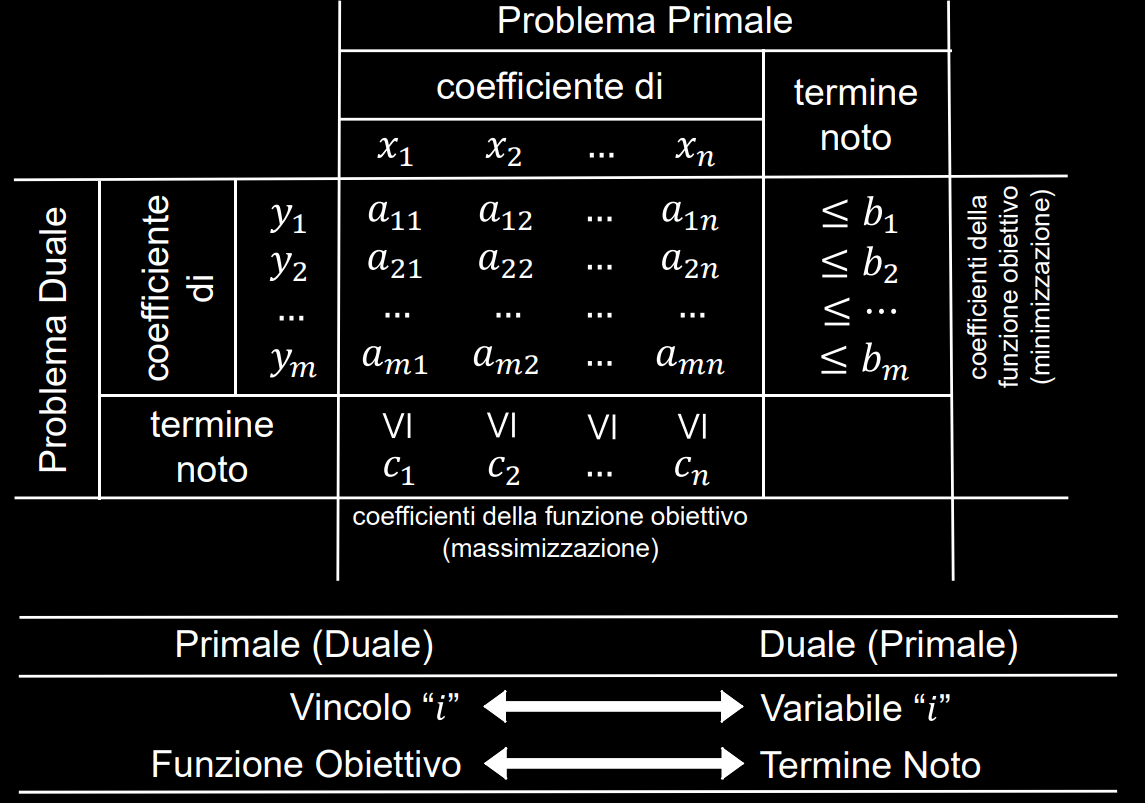
\includegraphics[width = 0.80\linewidth]{Images/46.png}
\end{center}
\subsubsection{Origine del duale}
Il contenuto della riga (0) del tableau, in corrispondenza di una generica iterazione del \textbf{metodo del simplesso} applicato al \textbf{problema primale}, è riportato di seguito:
\begin{center}
    \makebox[\textwidth]{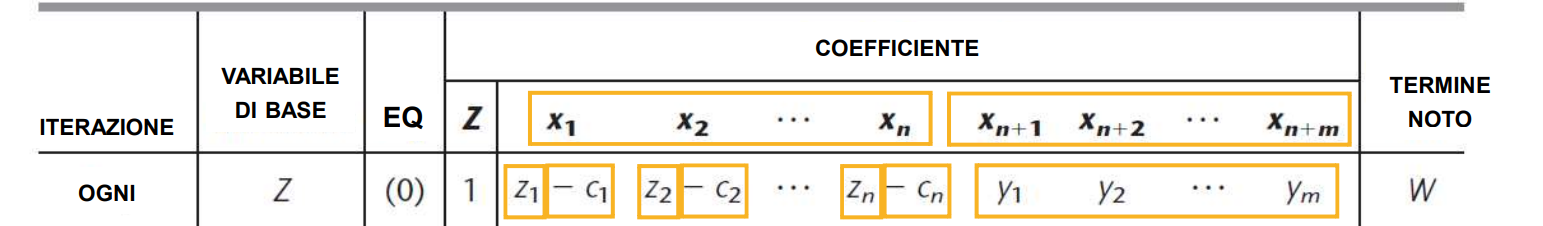
\includegraphics[width = 0.80\paperwidth]{Images/47.png}}
\end{center}
Si osservi che per i coefficienti di $x_1, x_2, ..., x_n$ con $\boldsymbol{z} = (z_1, z_2, ..., z_n)$ indichiamo con $-\boldsymbol{c}$ il vettore che il metodo del simplesso
ha sommato ai coefficienti iniziali per ottenere il tableau corrente.
Similmente dato che i coefficienti iniziali di $x_{n+1}, x_{n+2}, ..., x_{n+m}$ nella riga (0) sono tutti 0 nel tableau iniziale,
$\boldsymbol{y} = (y_1, y_2, ..., y_m)$ indica il vettore che il metodo del simplesso ha sommato a tali coefficienti.
Si può dimostrare che valgono le seguenti relazioni:
$$W = \boldsymbol{y}\boldsymbol{b} = \sum_{i=1}^m b_i \cdot y_i$$
$$\boldsymbol{z} = \boldsymbol{y}\boldsymbol{A} \Rightarrow z_j = \sum_{i=1}^m a_{ij} \cdot y_i, j = 1,2,...,n$$
Facciamo un esempio per chiarire il concetto: prendiamo in considerazione il seguente problema di PL:
\begin{equation*}
    \begin{array}{ll}
        \displaystyle \textrm{max} & \; Z = 3 \cdot x_1 + 5 \cdot x_2\\
        \textrm{s.a.} & x_1 \leq 4\\
        \phantom{} & 2 \cdot x_2 \leq 12\\
        \phantom{} & 3 \cdot x_1 + 2 \cdot x_2 \leq 18 \\
        \phantom{} & x_1,x_2 \geq 0
    \end{array}
\end{equation*}
Poiché il problema duale è esprimibile nel seguente modo:
\begin{equation*}
    \begin{array}{ll}
        \displaystyle \textrm{min} & \; W = \sum_{i=1}^m b_i \cdot y_i\\
        \textrm{s.a.} & \sum_{i=1}^m a_{ij} \cdot y_i \geq c_j, j= 1,...,n\\
        \phantom{} & y_i \geq 0, i=1,...,m
    \end{array}
\end{equation*}
Allora la \textbf{funzione obbiettivo del problema duale} è:
$$W = 4 \cdot y_1 + 12 \cdot y_2 + 18 \cdot y_3$$
I termini sinistri dei \textbf{vincoli del problema duale} si ottengono guardando i vincoli del problema primale "colonna per colonna":
$$z_1 = y_1 + 3 \cdot y_3$$
$$z_2 = 2 \cdot y_2 + 2 \cdot y_3$$
Pertanto, sottraendo i termini noti a destra dei vincoli di $\geq$, in questo caso $c_1 = 3$ e $c_2 =5$, allora
$(z_1 - c_1)$ e $(z_2 - c_2)$ sono interpretabili come \textbf{variabili di surplus} di questi vincoli funzionali, e risultano:
$$z_1 - c_1 = y_i + 3 \cdot y_3 - c_1$$
$$z_2 - c_2 = 2 \cdot y_2 + 2 \cdot y_3 - c_2$$
Esprimiamo ora, in termini simbolici, cosa cerca di ottenere il metodo del simplesso dal punto di vista del \textbf{test di ottimalità}. Il 
\textbf{metodo del simplesso}
\begin{itemize}
    \item Cerca un insieme di variabili di base, e la corrispondente soluzione ammissibile di base, tale che tutti i coefficienti della riga (0) siano non negativi
    \item Termina restituendo questa come soluzione ottimale
\end{itemize}
Adottando la notazione della tabella sopra, l'obbiettivo inseguito dal metodo del simplesso è esprimibile come segue:
\begin{center}
    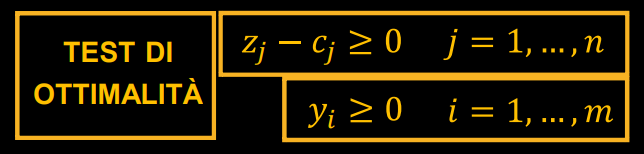
\includegraphics[width = 0.45\linewidth]{Images/48.png}
\end{center}
Sostituendo:
$$z_j = \sum_{i=1}^{m} a_{ij} \cdot y_i$$
in
$$z_j - c_j \geq 0, j = 1,...,n$$
$$y_i \geq 0, i = 1,...,m$$
e ricordando che
$$W = \sum_{i=1}^{m} b_i \cdot y_i$$
la condizione di ottimalità indica che il metodo del simplesso cerca i valori $y_1, y_2, ..., y_m$ tali che
$$W = \sum_{i=1}^{m} b_i \cdot y_i$$
$$\sum_{i=1}^{m} a_{ij} \cdot y_i \geq c_j, j= 1,...,n$$
$$y_i \geq 0, i = 1,...,m$$
Fatta eccezione per la mancanza del tipo di obbiettivo da ottimizzare per $W$, questo problema è \textbf{esattamente il problema duale}:
\begin{equation*}
    \begin{array}{ll}
        \displaystyle \textrm{min} & \; W = \sum_{i=1}^m b_i \cdot y_i\\
        \textrm{s.a.} & \sum_{i=1}^m a_{ij} \cdot y_i \geq c_j, j= 1,...,n\\
        \phantom{} & y_i \geq 0, i=1,...,m
    \end{array}
\end{equation*}
Per completare la formulazione, dovremmo mostrare come determinare il tipo di obbiettivo per $W$, cosa che affronteremo successivamente.
Il problema duale può allora essere visto come una diversa formulazione, in termini di PL, di quello che è l'obbiettivo del metodo del simplesso, vale a dire,
ottenere una soluzione del problema primale che soddisfi il test di ottimalità:
\begin{itemize}
    \item Prima di ottenere una soluzione del problema primale che soddisfi il test di ottimalità, il vettore riga $\boldsymbol{y}$ della riga (0) (coefficienti delle variabili di slack) del tableau corrente
    deve essere inammissibile per il problema duale ($y_1 < 0$ per qualche $i$)
    \item Ottenuta una soluzione del problema primale che soddisfi il test di ottimalità, il corrispondente vettore $\boldsymbol{y}$ della riga (0) deve essere una soluzione ottimale $\boldsymbol{y}^*$ per il problema duale,
    in quanto soluzione ammissibile che ottiene il minimo valore della funzione obbiettivo $W$
\end{itemize}
La soluzione ottimale $\boldsymbol{y}^* = (y_1^*, y_2^*, ..., y_m^*)$ fornisce i \textbf{prezzi ombra} del problema primale. Inoltre, il valore ottimale di $W$ \textbf{è il valore ottimale di $Z$}, pertanto i valori ottimali delle due funzioni obbiettivo,
primale e duale, \textbf{sono uguali}. Questo implica che $\boldsymbol{c}\boldsymbol{x} \leq \boldsymbol{y}\boldsymbol{b}$, per ogni $\boldsymbol{x}$ e $\boldsymbol{y}$ che siano ammissibili rispettivamente per il primale e per il duale.
\subsubsection{Relazione primale-duale}
Formalizziamo le relazioni Primale-Duale:
\begin{itemize}
    \item \textbf{Proprietà di dualità debole}: se $\boldsymbol{x}$ è una soluzione ammissibile per il problema primale e $\boldsymbol{y}$ è una soluzione ammissibile per il corrispondente problema duale, allora vale la seguente disuguaglianza:
    $$\boldsymbol{c}\boldsymbol{x} \leq \boldsymbol{y}\boldsymbol{b}$$
    \item \textbf{Proprietà di dualità forte}: se $\boldsymbol{x}^*$ è una soluzione ottimale per il problema primale e $\boldsymbol{y}^*$ è una soluzione ottimale per il corrispondente problema duale, allora vale la seguente uguaglianza:
    $$\boldsymbol{c}\boldsymbol{x}^* = \boldsymbol{y}^*\boldsymbol{b}$$
\end{itemize}
Queste due proprietà, se considerate insieme, implicano che la diseguaglianza vale per le soluzioni ammissibili se una o entrambe non sono ottimali per i corrispondenti problemi,
l'uguaglianza vale solo se entrambe sono soluzioni ottimali.
La \textbf{proprietà di dualità debole} descrive la relazione esistente tra ogni coppia di soluzioni, una del primale ed una del duale, nel caso in cui entrambe siano ammissibili per i rispettivi problemi.
Ad ogni iterazione, il metodo del simplesso trova una specifica coppia di soluzioni per i due problemi, dove la soluzione del primale è ammissibile mentre quella del duale non è ammissibile, fatta eccezione per l'ultima iterazione, quella che vede l'arresto del metodo del simplesso.
La proprietà che enunciamo di seguito descrive situazione e relazione tra coppie di soluzioni, primale/duale:
\begin{itemize}
    \item \textbf{Proprietà delle soluzioni complementari}: ad ogni iterazione, il metodo del simplesso identifica simultaneamente una soluzione vertice ammissibile $\boldsymbol{x}$ per il problema primale
    e una soluzione complementare $\boldsymbol{y}$ per il problema duale (reperibile nella riga (0), i coefficienti delle variabili di slack), dove
    $$\boldsymbol{c}\boldsymbol{x} = \boldsymbol{y}\boldsymbol{b}$$
    Se $\boldsymbol{x}$ non è ottimale per il problema primale, allora $\boldsymbol{y}$ non è ammissibile per il problema duale
    \item \textbf{Proprietà delle soluzioni ottimale complementari}: all'iterazione finale, il metodo del simplesso identifica simultaneamente una soluzione ottimale $\boldsymbol{x}^*$ per il problema primale e una soluzione
    ottimale complementare $\boldsymbol{y}^*$ per il problema duale (reperibile nella riga (0), i coefficienti delle variabili di slack), dove
    $$\boldsymbol{c}\boldsymbol{x}^* = \boldsymbol{y}^*\boldsymbol{b}$$
\end{itemize}
Le componenti $y_i^*$ sono i \textbf{PREZZI OMBRA DEL PROBLEMA PRIMALE}.
Un'altra proprietà interessante è la seguente:
\begin{itemize}
    \item \textbf{Proprietà di simmetria}: per ogni problema primale e relativo problema duale, tutte le relazioni tra loro debbono essere simmetriche in quanto, come vedremo successivamente, il problema duale del problema duale è il problema primale
\end{itemize}
Questo significa che le proprietà di dualità debole, di dualità forte, di soluzioni complementari, di soluzioni ottime complementari, sono valide sia per il problema primale che il corrispondete problema duale.
Sino ad ora, abbiamo focalizzato l'attenzione alle relazioni tra soluzioni ammissibili o ottimali del problema primale e le corrispondenti soluzioni del problema duale.
Comunque, è possibile che il problema primale (duale) non abbia soluzioni ammissibili o abbia soluzioni ammissibili ma non soluzioni ottimali (funzione obbiettivo illimitata).
L'ultima proprietà che presentiamo, riassume le relazioni primale-duale in tutti i casi possibili:
\begin{itemize}
    \item \textbf{TEOREMA DI DUALITÀ}: le sole relazioni possibili tra problema primale e duale sono le seguenti:
    \begin{enumerate}
        \item Se un problema ha \textbf{soluzioni ammissibili} e \textbf{funzioni obbiettivo limitata} (pertanto tale da avere soluzione ottimale), allora la stessa cosa vale per il problema duale, per cui sia la proprietà debole della dualità che la proprietà forte della dualità sono applicabili
        \item Se un problema ha \textbf{soluzioni ammissibili} e \textbf{funzione obbiettivo illimitata} (pertanto tale da non avere soluzione ottimale), allora l'altro problema non ha soluzioni ammissibili
        \item Se un problema \textbf{non ha soluzioni ammissibili}, allora l'altro problema o non ha soluzioni ammissibili o ha una funzione obbiettivo illimitata
    \end{enumerate}
\end{itemize}
\subsubsection{Interpretazione del duale}
L'interpretazione economica della dualità è basata sull'interpretazione del problema primale in \textbf{forma standard} che abbiamo presentato precedentemente e che riportiamo di seguito per comodità:
\begin{itemize}
    \item $Z =$ valore della misura di prestazione
    \item $x_j =$ livello di attività $"j"$
    \item $c_j =$ incremento del valore della misura di prestazione $Z$ corrispondente all'incremento di un'unità del valore dell'attività $x_j$
    \item $b_i =$ quantità di risorsa $"i"$ allocabile alle attività $x_j, j = 1,...,n$
    \item $a_{ij} =$ quantità di risorsa $"i"$ consumata da ogni unità di attività $x_j, j = 1,...,n$
\end{itemize}
Il problema di programmazione lineare è quindi formulabile come:
\begin{equation*}
    \begin{array}{ll}
    \displaystyle \textrm{max} & \; Z = c_1 \cdot x_1 + c_2 \cdot x_2 +...+ c_n \cdot x_n\\
    \textrm{s.a.} & a_{11} \cdot x_1 + a_{12} \cdot x_2 +...+ a_{1n} \cdot x_n \leq b_1 \\
    \phantom{} & a_{21} \cdot x_1 + a_{22} \cdot x_2 +...+ a_{2n} \cdot x_n \leq b_2 \\
    \phantom{} &... ... ... + ... ... ... + ... + ... ... ... \leq ... \\
    \phantom{} & a_{m1} \cdot x_1 + a_{m2} \cdot x_2 +...+ a_{mn} \cdot x_n \leq b_m \\
    \phantom{} &x_1 \geq 0, x_2 \geq 0, x_3 \geq 0 ..., x_m \geq 0
    \end{array}
\end{equation*}
Per mostrare come l'interpretazione del primale conduca all'interpretazione economica del duale, osserviamo che il valore di $W$ è uguale al valore del profitto totale $Z$, ($W = Z$), (\textbf{PROPRIETÀ DELLE SOLUZIONI COMPLEMENTARI})
ad ogni iterazione corrente del metodo del simplesso.
Siccome $W = b_1 \cdot y_1 + b_2 \cdot y_2 + ... + b_m \cdot y_m$, ogni $b_i \cdot y_i$ è interpretabile come contributo corrente al profitto
$Z = W$ se $b_i$ unità di risorse $"i"$ sono rese disponibili per il primale. Pertanto \textbf{la variabile duale $y_i$ è interpretata come il contributo al profitto per unità di risorsa $"i"$, quando il corrente insieme di variabili di base viene utilizzato per ricavare la soluzione del primale}.
In altri termini, i valori $y_i$ (o $y_i^*$ nel caso di soluzione ottimale) sono i \textbf{PREZZI OMBRA}.
Consideriamo il problema che abbiamo presentato come esempio fino ad ora: 
\begin{center}
    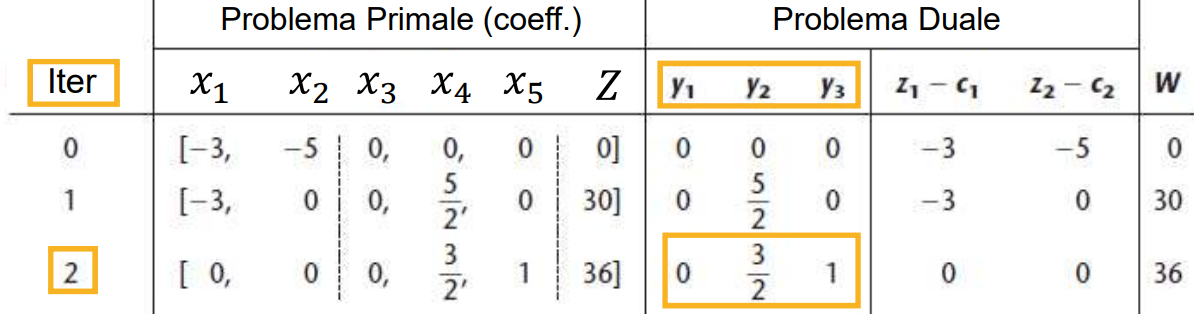
\includegraphics[width = 1\linewidth]{Images/49.png}
\end{center}
\noindent
all'iterazione $2$ il metodo del simplesso trova la soluzione ottimale, e trova allo stesso tempo il valore ottimale delle variabili duali
$\underbrace{y_1^* = 0, y_2^* = \frac{3}{2}, y_3^* = 1}_{\textrm{Prezzi ombra}}$.
Essi indicano che aumentando individualmente ogni termine $b_i$ di un'unità (1), il valore ottimale della funzione obbiettivo (profitto) aumenta di $y_i^*$.
Pertanto, $y_i^*$ è interpretabile come \textbf{contributo al profitto per unità di risorsa $"i"$ se si utilizza la soluzione ottimale}.
Questa interpretazione delle variabili duali porta ad una conseguente interpretazione dell'intero problema duale. Nello specifico, dato che ogni unità di attività $"j"$ del problema
primale consuma $a_{ij}$ unità della risorsa "i", allora $\sum_{i=1}^m a_{ij} \cdot y_i$ è interpretabile come \textbf{il contributo corrente al profitto}, del mix di risorse che verrebbero consumate,
\textbf{se un'unità (1) di attività "j" venisse utilizzata ($j = 1, 2, ..., n$)}.
Per ogni attività $"j"$, lo stesso mix di risorse può probabilmente essere utilizzato in modi differenti, ma nessun utilizzo alternativo che risulti meno "profittevole" di 1 unità dell'attività "$j$" dovrebbe essere
considerato come potenziale alternativa. Dato che $c_j$ è interpretato come il \textbf{profitto unitario per l'attivita $"j"$}, allora ogni \textbf{vincolo funzionale del problema duale} viene interpretato come segue:
$\sum_{i=1}^{m} a_{ij} \cdot y_i \geq c_j$; dice che il contributo effettivo al profitto del mix di risorse deve essere almeno pari a quello che si otterrebbe nel caso di un'unità (1) di attività $"j"$; altrimenti, saremmo
nelle condizioni non utilizzare al meglio quelle risorse.
Per il problema presentato come esempio, i profitti unitari sono $c_1 =3$ e $c_2 = 5$, pertanto i vincoli funzionali del duale, interpretabili come sopra, sono
$$y_1 + 3 \cdot y_3 \geq 3$$
$$2 \cdot y_2 + 2 \cdot y_2 \geq 5$$
In modo similare, \textbf{l'interpretazione dei vincoli di non negatività} è enunciabile come segue:
$y_i \geq 0$; indica che il \textbf{contributo al profitto della risorsa $"i" (i = 1, 2, ..., m)$ deve essere non negativo}: altrimenti, risulterebbe meglio \textbf{non utilizzare la risorsa $"i"$}.
L'obbiettivo:
$$\textrm{min} \; W = \sum_{i=1}^{m}b_i \cdot y_i$$
può essere interpretato come la \textbf{minimizzazione del valore implicito di tutte le risorse consumate dalle attività}. Per il problema d'esempio, il valore implicito totale delle risorse consumate dai due prodotti è pari a
$$W = 4 \cdot y_1 + 12 \cdot y_2 + 18 \cdot y_3$$
\subsubsection{Proprietà delle soluzioni di base complementari}
La prima relazione primale-duale che presentiamo estende la \textbf{proprietà delle soluzioni complementari}, introdotta precedentemente, alla \textbf{forma aumentata} del problema primale e del problema duale e successivamente ad \textbf{ogni soluzione di base}
(ammissibile o meno) del problema primale.
\begin{itemize}
    \item \textbf{PROPRIETÀ DELLE SOLUZIONI DI BASE COMPLEMENTARI}: ogni soluzione di base del primale ha una soluzione di base complementare nel problema duale, in modo tale che i rispettivi valori delle funzioni obbiettivo $Z$ e $W$ \textbf{siano uguali}.
    Data la riga (0) del tableau del simplesso per la soluzione di base primale, la soluzione di base complementare del duale $(\boldsymbol{y},\boldsymbol{z} - \boldsymbol{c})$ viene ricavata come di seguito:
    \begin{center}
        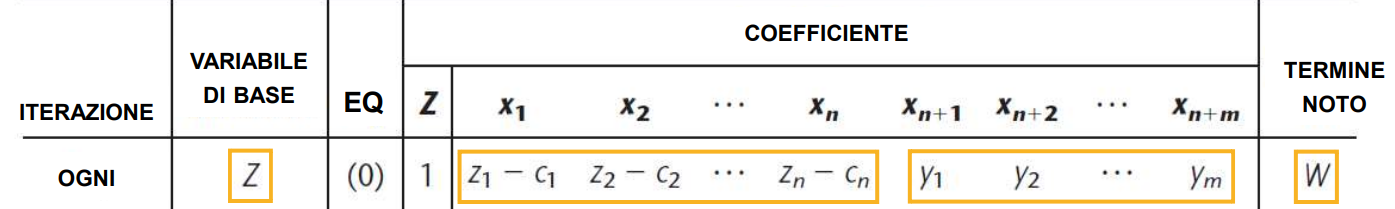
\includegraphics[width = 1\linewidth]{Images/50.png}
    \end{center}
\end{itemize}
\subsubsection{Proprietà di complenetary slackness}
La prossima proprietà mostra come identificare quali siano le variabili di base e quali siano le variabili non di base a partire da un soluzione di base complementare.
\begin{itemize}
    \item \textbf{PROPRIETÀ DI COMPLEMENTARY SLACKNESS}: data l'associazione tra variabili riporta nella seguente tabella 
    \begin{center}
        \includegraphics[width = 1\linewidth]{Images/51.png}
    \end{center}
    le variabili della soluzione di base del primale e la soluzione di base complementare del duale soddisfano la relazione di \textbf{complementary slackness} mostrata nella tabella qui sotto
    \begin{center}
        \includegraphics[width = 0.60\linewidth]{Images/52.png}
    \end{center}
    Inoltre, questa relazione \textbf{è simmetrica}, facendo in modo che due soluzioni di base siano \textbf{reciprocamente complementari}.
\end{itemize}
Utilizziamo il problema d'esempio per mostrare le due proprietà fino a qui presentate:
ricordiamo che il problema primale è:
\begin{equation*}
    \begin{array}{ll}
        \displaystyle \textrm{max} & \; Z = 3 \cdot x_1 + 5 \cdot x_2\\
        \textrm{s.a.} & x_1 \leq 4\\
        \phantom{} & 2 \cdot x_2 \leq 12\\
        \phantom{} & 3 \cdot x_1 + 2 \cdot x_2 \leq 18 \\
        \phantom{} & x_1,x_2 \geq 0
    \end{array}
\end{equation*}
quindi il suo problema duale è:
\begin{equation*}
    \begin{array}{ll}
        \displaystyle \textrm{min} & \; W = 4 \cdot y_1 + 12 \cdot y_2 + 18 \cdot y_3\\
        \textrm{s.a.} & y_1 + 3 \cdot y_3 \geq 3\\
        \phantom{} & 2 \cdot y_2 + 2 \cdot y_3 \geq 5\\
        \phantom{} & y_1,y_2, y_3 \geq 0
    \end{array}
\end{equation*}
Consideriamo la seguente tabella:
\begin{center}
    \includegraphics[width = 1\linewidth]{Images/53.png}
\end{center}
Le 8 soluzioni di base (5 ammissibili e 3 inammissibili) del problema primale sono mostrare a destra,
pertanto il corrispettivo problema duale deve avere 8 soluzioni di base, ognuna complementare ad una delle soluzioni di base primali.
Per ogni soluzione di base del primale, la \textbf{proprietà di complementary slackness} può essere usata per identificare le variabili di base
e quelle non di base della sua soluzione di base complementare, in modo tale che la soluzione complementare risolva il seguente sistema di equazioni:
$$z_j - c_j = \sum_{i=1}^{m} a_{ij} \cdot y_i - c_j, j = 1, 2, ..., n$$
\noindent 
la tabella sopra mostra le soluzioni di base ammissibili trovate applicando il metodo del simplesso al problema primale.
\subsubsection{Relazioni tra soluzioni di base complementari}
Estendiamo ora la \textbf{proprietà delle soluzioni ottimali complementari} alla \textbf{forma aumentata} dei due problemi (primale/duale).
\begin{itemize}
    \item \textbf{PROPRIETÀ DELLE SOLUZIONI OTTIMALI COMPLEMENTARI}: una soluzione di base ottimale $\boldsymbol{x}^*$ del problema primale ha una soluzione
    di base ottimale complementare del duale, tale che i valori delle rispettive funzioni obbiettivo ($Z$ e $W$) \textbf{sono identici} ($Z = W$). Data la riga (0) del
    tableau del metodo del simplesso, corrispondente alla soluzione ottimale del primale $\boldsymbol{x}^*$, la soluzione ottimale complementare del duale
    $(\boldsymbol{y}, \boldsymbol{z}^* - \boldsymbol{c})$ viene ricavata come mostrato nella tabella sottostante:
    \begin{center}
        \includegraphics[width = 1\linewidth]{Images/54.png}
    \end{center}
\end{itemize}
Analizziamo nel dettaglio il ragionamento sottostante a questa proprietà: notiamo che la soluzione duale $(\boldsymbol{y}^*, \boldsymbol{z}^* - \boldsymbol{c})$ deve essere ammissibile per il duale
in quanto la \textbf{condizione di ottimalità di $\boldsymbol{x}^*$ per il primale} impone che tutte le variabili duali (incluse le variabili surplus) siano non negative.
Dato che questa soluzione $(\boldsymbol{y}^*, \boldsymbol{z}^* - \boldsymbol{c})$ è ammissibile, deve essere ottimale per il duale in forma della \textbf{proprietà di dualità debole}.
Le soluzioni di base sono classificabili in base al fatto che soddisfino o meno ciascuna delle seguenti condizioni:
\begin{itemize}
    \item \textbf{CONDIZIONE DI AMMISSIBILITÀ}: vale a dire se tutte le variabili (incluse le variabili di slack della soluzione aumentata) sono non negative
    \item \textbf{CONDIZIONE DI OTTIMALITÀ}: vale a dire se i coefficienti nella riga (0) (tutte le variabili della soluzione di base complementare) sono non negativi
\end{itemize}
I nomi che useremo per i differenti tipi di soluzioni di base sono riassunti nella tabella seguente:
\begin{center}
    \includegraphics[width = 1\linewidth]{Images/55.png}
\end{center}
Le relazioni tra le soluzioni di base complementari vengono riassunte qui sotto:
\begin{center}
    \includegraphics[width = 1\linewidth]{Images/56.png}
\end{center}
\newpage \noindent
I possibili valori delle funzioni obbiettivo ($Z = W$) per le prime tre coppie di esiti della tabella sopra sono illustrati qui sotto:
\begin{center}
    \includegraphics[width = 0.80\linewidth]{Images/57.png}
\end{center}
Nella figura soprastante è possibile constatare che il mentre il \textbf{metodo del simplesso} visita soluzioni di base \textbf{sub-ottimali}, cercando di trovare la soluzione ottimale del problema primale,
indirettamente è come se \textbf{visitasse soluzioni complementari super-ottimali}, cercando di ottenere una soluzione ammissibile per il problema duale. In alcuni casi può essere vantaggioso o necessario \textbf{lavorare direttamente con soluzioni di base super-ottimali},
cercando di ottenere l'ammissibilità del problema primale, questo è l'approccio seguito dal \textbf{metodo del simplesso duale} che tuttavia non tratteremo.
Nella tabella che mostrava le relazioni tra soluzioni di base complementari, le due ultime colonne introducono altrettanti termini comuni che vengono utilizzati per descrivere una \textbf{COPPIA DI SOLUZIONI DI BASE COMPLEMENTARI}, che vengono dette:
\begin{itemize}
    \item \textbf{PRIMALE AMMISSIBILE}: se la soluzione di base primale è ammissibile per il primale
    \item \textbf{DUALE AMMISSIBILE}: se la soluzione di base complementare del duale è ammissibile per il duale
\end{itemize}
Utilizzando questa terminologia, il metodo del simplesso visita soluzioni \textbf{PRIMALI AMMISSIBILI}, cercando di ottenere l'ammissibilità del duale.
Quanto questo viene ottenuto, le due soluzioni di base complementari sono ottimali per i rispettivi problemi.
\subsubsection{Adattamento ad altre forme primali}
Fino ad ora abbiamo implicitamente assunto che il problema primale fosse in forma standard. Comunque, ad ogni problema di PL, in qualunque forma sia, corrisponde una forma duale.
Abbiamo già visto come ogni problema di programmazione lineare possa essere ricondotto alla corrispondente forma standard. Pertanto, è sempre possibile trasformare un problema dalla forma
\textbf{forma non standard} alla corrispondente \textbf{forma standard}. Ottenuta la forma standard è poi possibile ottenere il problema duale del problema in tale forma.
Dato che ogni coppia di problemi primale/duale è convertibile come mostrato sotto:
\begin{center}
    \includegraphics[width = 0.60\linewidth]{Images/58.png}
\end{center}
questo implica che il \textbf{il duale del problema duale è il problema primale}. Pertanto, tutte le relazioni esistenti tra un problema primale e il relativo problema duale devono essere
simmetriche (\textbf{PROPRIETÀ DI SIMMETRIA}, che ora diviene chiaro perché sia valida).
Una prima conseguenza della \textbf{PROPRIETÀ DI SIMMETRIA} è che tutte le affermazioni fatte nelle lezioni precedenti circa le relazioni tra problema duale e problema primale sono valide anche dal problema
primale al problema duale. Inoltre, diviene chiaro come non abbia senso preoccuparsi di quale problema venga chiamato primale e quale problema venga chiamato duale.
Tipicamente si usa la convenzione che il problema formulato per rappresentare il problema che desideriamo risolvere viene chiamato problema primale, indipendentemente dalla sua forma.
Abbiamo appena mostrato come trasformare un problema primale in forma non standard nel corrispondente problema duale in forma standard. Tuttavia, nella forma non standard del problema primale
\textbf{non erano presenti vincoli di eguaglianza o variabili decisionali non vincolate in segno}.
Effettivamente, per queste due particolari forme (vincoli di eguaglianza o variabili decisionali non vincolate in segno) esiste una scorciatoia: il \textbf{metodo SOB}.
\newpage
\subsubsection{Metodo Sensible-Odd-Bizarre}
Il \textbf{metodo SOB (Sensibile-Odd-Bizarre)} è descrivibile come segue:
\begin{enumerate}
    \item Se il problema è formulato in termini di \textbf{massimizzazione} o \textbf{minimizzazione}, il problema duale sarà automaticamente nell'altra forma. ($min \rightarrow max, max \rightarrow min$)
    \item Etichettare le diverse forme di \textbf{vincoli funzionali ed i vincoli sulle singole variabili decisionali del primale} come \textbf{Sensible, Odd e Bizarre}, in accordo alla tabella sotto riportata
    \begin{center}
        \includegraphics[width = 0.60\linewidth]{Images/59.png}
    \end{center}
    L'etichettature dei vincoli funzionali dipende dal tipo di problema (max o min).
    \item Per ogni \textbf{vincolo su una variabile di decisione del problema duale}, utilizzare la forma che ha medesima etichetta del \textbf{vincolo funzionale per il problema primale} corrispondente
    a questa variabile duale secondo la tabella qui sotto:
    \begin{center}
        \includegraphics[width = 0.60\linewidth]{Images/60.png}
    \end{center}
    \item Per ogni \textbf{vincolo funzionale del problema duale}, utilizzare la forma che ha la stessa etichetta del \textbf{vincolo della corrispondente variabile di decisione del problema primale} (tabella sopra)
\end{enumerate}
\section{Programmazione lineare intera}
Fino ad ora abbiamo visto diversi esempi delle numerose e diverse applicazioni delle programmazione lineare.
Una limitazione chiave che non abbiamo ancora affrontato è \textbf{l'ipotesi di divisibilità}, che richiede che le variabili decisionali siano 
del dominio reale. In molti problemi pratici, tuttavia, le variabili di decisione effettivamente hanno senso solo se hanno valori interi, come abbiamo visto in alcune applicazioni come
assegnamento, trasporto o problemi di flusso su reti.
In generale se si richiede che le variabili di decisione assumano valori interi allora si parla di \textbf{Programmazione Lineare Intera} (PLI).
Se solo alcune delle variabili di decisione devono essere intere allora si parla di \textbf{Programmazione Lineare Mista} (PLM).
\subsection{Ottimizzazione Intera e Binaria}
Consideriamo un generico problema di programmazione lineare con $n$ variabili e $m$ vincoli:
$$\textrm{opt } f(\boldsymbol{v}) = \boldsymbol{c}^T\boldsymbol{x} \; \; \textrm{(funzione obbiettivo lineare)}$$
$$X = \left \{ \boldsymbol{x}: g_i(\boldsymbol{x} \begin{Bmatrix}
    \geq \\
    = \\
    \leq
\end{Bmatrix}) 0, i = 1,...,m \right \} \; \; \textrm{con } g_i(\boldsymbol{x}) = \boldsymbol{a}_i^T\boldsymbol{x} - b_i \; \textrm{(vincoli lineari)}$$
dove $\boldsymbol{a} \in \mathbb{R}^n, \boldsymbol{b} \in \mathbb{R}^m$ e $\boldsymbol{c} \in \mathbb{R}^n$ e $opt = \begin{Bmatrix}
    min \\
    max
\end{Bmatrix}$
Se $\boldsymbol{x} \in \mathbb{Z}^n$ abbiamo un problema di \textbf{programmazione lineare intera} (PLI). \newline
Se $\boldsymbol{x} \in \{0,1\}^n$ abbiamo un problema di \textbf{programmazione lineare binaria} (PB) \newline
Se $\boldsymbol{x} \in \mathbb{R}^p \times \mathbb{Z}^q$ con $p + q = n$ e $p > 0$ e $q > 0$ abbiamo un problema di \textbf{Programmazione Lineare Mista} (PLM), o
\textbf{Mixed Integer Programming} (MIP).
Avendo solo variabili di decisione binarie, il numero di soluzioni è $2^n$.
\subsubsection{Modellazione con variabili binarie}
Le variabili binarie trovano un vasto impiego in Ricerca Operativa per modellare le decisioni di tipo "Si o No?"
Le variabili binarie permettono di introdurre condizioni logiche: \newline
\begin{itemize}
    \item \textbf{Vincoli di tipo "either-or"}: Consideriamo il caso in cui, dati due vincoli, almeno uno di questi deve essere soddisfatto (per esempio perché
    potrebbe esserci una scelta su risorse alternative da utilizzare per un determinato scopo, in modo che sia necessario solo uno dei due vincoli). Per esempio:
    $$3x_1 + 2x_2 \leq 18 \; textrm{oppure } x_1 + 4x_2 \leq 16$$
    La formulazione sopra risulta equivalente al seguente insieme di vincoli:
    $$\begin{cases}
        3x_1 + 2x_2 \leq 18 + My \\
        x_1 + 4x_2 \leq 16 + M(1-y)
    \end{cases}$$
    con $M$ numero positivo molto grande e $y \in \{0,1\}$.
    Infatti:
    \begin{itemize}
        \item Se $y = 0$ allora $3x_1 + 2x_2 \leq 18$ rimane mentre $x_1 + 4x_2 \leq 16 + M$ è sempre soddisfatto per $M$ molto grande quindi può essere eliminato.
        \item Se $y = 1$ allora $x_1 + 4x_2 \leq 16$ rimane mentre $3x_1 + 2x_2 \leq 18 + M$ è sempre soddisfatto per $M$ molto grande e quindi può essere eliminato.
    \end{itemize}
    \item \textbf{Dati $N$ vincoli, solo $K$ di questi sono presenti}: Consideriamo il caso in cui un modello includa $N$ vincoli tali che solo $K$ devono essere soddisfatti (con $K < N$):
    $$f_1(x_1, x_2, ..., x_n) \leq d_1$$
    $$f_2(x_1, x_2, ..., x_n) \leq d_2$$
    $$...$$
    $$f_N(x_1, x_2, ..., x_n) \leq d_N$$
    Consideriamo $N$ variabili binarie $y_i \in \{0,1\}$ per $i = 1,...,N$ ed un numero $M$ positivo molto grande.
    Abbiamo la seguente formulazione equivalente al requisito che solo $K$ di questi $N$ vincoli devono essere soddisfatti:
    $$\begin{cases}
        f_1(x_1, x_2, ..., x_n) \leq d_1 + My_1 \\
        f_2(x_1, x_2, ..., x_n) \leq d_2 + My_2 \\
        ... \\
        f_N(x_1, x_2, ..., x_n) \leq d_N + My_N \\
        \sum_{i=1}^{N} y_i = N - K
    \end{cases}$$
    \item \textbf{La funzione assume solo $N$ possibili valori}: Si consideri la situazione in cui una data funzione assuma uno fra $N$ possibili valori.
    $$f(x_1, x_2, ..., x_n) = d_1 \; o \; d_2 \; o ,..., \o \; d_N$$
    Ad esempio:
    $$f(x_1, x_2, ..., x_n) = \sum_{j=1}^{n} a_jx_j$$
    oppure
    $$f(x_1, x_2, ..., x_n) = x_j$$
    Consideriamo $N$ variabili binarie $y_i \in \{0,1\}$ per $i = 1,...,N$.
    Abbiamo la seguente formulazione equivalente al requisito che una data funzione assuma uno fra $N$ possibili valori:
    $$\begin{cases}
        f(x_1, x_2, ..., x_n) = \sum_{i=1}^{N} d_i y_i \\
        \sum_{i=1}^{N} y_i = 1
    \end{cases}$$
    \item \textbf{Problema del costo fisso}: Supponiamo che si voglia intraprendere un'attività $j$ il cui costo sia caratterizzato dalla seguente funzione:
    $$f(x) = \begin{cases}
        k + cx & \textrm{se } x > 0 \\
        0 & \textrm{se } x = 0
    \end{cases}$$
    dove $k > 0$ denota il \textbf{costo fisso}, $x \geq 0$ è il livello di attività e $c$ è il costo per ogni unità incrementale.
    La minimizzazione di tale funzione può essere espressa attraverso il seguente modello PLI:
    $$\textrm{min } z = (ky + cx)$$
    soggetto ai seguenti vincoli:
    $$\begin{cases}
        x - My \leq 0 & \textrm{o equivalentemente } x \leq My \\
        y \in \{0,1\} \; e \; x \geq 0
    \end{cases}$$
    dove $M$ denota un numero molto grande. Notiamo che:
    \begin{itemize}
        \item Se $y = 0$ allora si ha $x leq 0 \rightarrow x = 0 \; e \; z = 0$
        \item Se $y = 1$ allora $x \leq M$, ovvero $x$ può assumere un qualsiasi valore, e $z = k + cx$
    \end{itemize}
    \item \textbf{Rappresentazioni binarie di variabili intere generiche}: Si supponga di avere un problema PLI puro (solo variabili intere)
    dove tutte le variabili sono \textbf{binarie} eccetto una. Supponiamo che tale variabile intera $x$ abbia valore nell'intervallo $[0,u]$. Chiamiamo $N$ quell'intero tale che:
    $$2^N \leq u \leq 2^{N+1}$$
    La rappresentazione binaria di $x$ è data da:
    $$x = \sum_{i = 0}^{N} 2^i y_i$$
    con $y_i$ variabili binarie aggiuntive.
    Sostituendo nel modello $x$ con tale rappresentazione è possibile passare ad un problema caratterizzato solo da variabili binarie.
    Facciamo un esempio: si supponga che un problema di PLI abbia tutte le variabili binarie eccetto due, $x_1$ e $x_2$ e che debba soddisfare i vincoli:
    $$x_1 \leq 5$$
    $$2x_1 + 3x_2 \leq 30$$
    Questo implica che $u_1 = 5$ e $u_2 = 10$ ovvero:
    $$2^2 \leq u_1 \leq 2^3$$
    $$2^3 \leq u_2 \leq 2^4$$
    Quindi
    $x_1 = y_0 + 2y_1 + 4y_2$ e $x_2 = y_3 + 2y_4 + 4y_5 + 8y_6$
    I vincoli del problema diventando quindi:
    $$y_0 + 2y_1 + 4y_2 \leq 5$$
    $$2y_0 + 4y_1 + 8y_2 + 3y_3 + 6y_4 + 12y_5 + 24y_6 \leq 30$$
\end{itemize}
\subsection{Considerazioni sui problemi di PLI}
Apparentemente, i problemi di PLI potrebbero risultare più facili da risolvere rispetto ai problemi di PL.
Un possibile ragionamento potrebbe essere:
\begin{itemize}
    \item I problemi di PL possono essere risolti efficientemente tramite il metodo del Simplesso
    \item Un problema di PLI è simile ad un problema PL eccetto che il numero di soluzioni di un problema PLI è molto minore
    \item Inoltre, i problemi di PLI con regione ammissibile limitata ai punti interi hanno un numero finito di soluzioni ammissibili
\end{itemize}
Quindi i problemi di PLI sono effettivamente più facili da risolvere? \textbf{ASSOLUTAMENTE NO!} Vediamo il perché:
\begin{enumerate}
    \item Il fatto di avere un numero finito di soluzioni ammissibili non assicura che un problema PLI sia facilmente risolvibile.
    Nel caso di un PLI con $n$ variabili binarie, ho $2^n$ soluzioni possibili da considerare, ovvero il numero di soluzioni \textbf{cresce esponenzialmente} con il numero di variabili da considerare.
    Se per esempio ho $n = 20$ variabili ho più di un milione di soluzioni possibili.
    \item La rimozione di alcune soluzioni ammissibili (quelle non intere) da un problema di PL non lo rende più semplice. Nel metodo del simplesso risulta fondamentale che le variabili possano assumere valori continui.
    Altrimenti non è possibile garantire l'esistenza di vertici ammissibili e quindi di soluzioni ammissibili di base.
\end{enumerate}
\subsection{Il metodo del rilassamento lineare}
Per un qualsiasi problema di PLI è possibile formulare il corrispettivo problema di PL, ovvero lo stesso problema senza i vincoli di interezza.
Tale problema prende il nome di \textbf{rilassamento lineare}.
\begin{center}
    \includegraphics[width = 1\linewidth]{Images/61.png}
\end{center}
\begin{center}
    \includegraphics[width = 1\linewidth]{Images/62.png}
\end{center}
Quando si affronta un problema di PLI è comune partire risolvendo il suo rilassamento lineare allo scopo di verificare se la soluzione
ottima trovata sia intera, nel qual caso abbiamo trovato la soluzione ottima. In caso contrario, si ottiene comunque un upper (lower) bound per problemi di max (min).
Vi sono casi particolari in cui risolvere un problema di PLI non è più difficile da risolvere del problema di PL associato ad esso, ovvero
quando la soluzione ottima del problema rilassato è una soluzione intera. In questo caso la soluzione del rilassamento lineare
DEVE necessariamente essere ottima anche per il problema di PLI. \newline
\textbf{ATTENZIONE}: in generale, la soluzione ottima di un problema di PLI può non corrispondere ad una delle sue soluzioni intere ottenute arrotondando le variabili non intere
(per esempio all'intero più vicino) del problema di PL associato:
\begin{center}
    \includegraphics[width = 1\linewidth]{Images/64.png}
\end{center}
Inoltre, una soluzione ottima del problema di PL associato non è necessariamente ammissibile per il problema di PLI dopo l'arrotondamento:
\begin{center}
    \includegraphics[width = 1\linewidth]{Images/63.png}
\end{center}
Nell'esempio sopra, la soluzione ottima del rilassamento lineare è il punto $(\frac{3}{2}, 2)$. Le soluzioni ottenute approssimando $x_1 = \frac{3}{2}$ all'intero più vicino
sono tuttavia \textbf{entrambe non ammissibili}.
\subsection{Metodo del Branch and Bound}
Il metodo del Branch and Bound è una tecnica generale per la risoluzione di problemi di ottimizzazione intera.
Proposto da A.H. Land e A.G. Doig nel 1960 per risolvere problemi di PLI, inizialmente venne sviluppato per risolvere
modelli di programmazione intera per il trasporto e lo stoccaggio del petrolio.
La tecnica del Branch and Bound è una tecnica di \textbf{enumerazione implicita}:
\begin{itemize}
    \item "Valuta" le soluzioni possibili fino a trovare quella ottima
    \item Scarta alcune di queste soluzioni a priori, dimostrando la loro non ottimalità 
    \item Si basa sul concetto di \textit{dividi et impera}
\end{itemize}
Ancora oggi il metodo del Branch and Bound rappresenta una delle tecniche più usate per risolvere i problemi di PL intera, binaria e mista.
\subsubsection{Funzionamento del metodo Branch and Bound}
Supponiamo di avere un problema di PLI:
$$max z = \boldsymbol{c}^T\boldsymbol{x} \; \textrm{(funzione obbiettivo lineare)}$$
$$X = \left \{ \boldsymbol{x} \in \mathbb{Z}^n : g_i(\boldsymbol{x}) \begin{Bmatrix}
    \geq \\
    = \\
    \leq
\end{Bmatrix} 0, i = 1,...,m \right \}$$
dove $\boldsymbol{a} \in \mathbb{R}^n, b \in \mathbb{R}^m$ e $c \in \mathbb{R}^n$. \newline
Indichiamo tale problema come \textbf{problema completo}. Un problema di PLI rappresenta un \textbf{sotto-problema} del problema completo se presenta la
\textbf{medesima funzione obbiettivo} ma ha un sottoinsieme proprio di $X$ come regione ammissibile.
Sia $z^* = f(x^*)$ la soluzione ottima del problema completo e $\tilde{z} = f(\tilde{x})$ la soluzione ottima di un sotto-problema,
allora si ha che $f(\tilde{x}) \leq f(x^*)$. Bisogna inoltre notare che tra le soluzioni ammissibili del problema completo vi è anche $\tilde{x}$ e che per definizione
di ottimo $f(\tilde{x}) \leq f(x^*)$. \newline
\textbf{ATTENZIONE}: per un problema di minimo \textbf{vale il contrario di quello esposto sopra}. \newline
Il Branch and Bound fa uso delle tre seguenti tecniche per risolvere un generico problema di PLI:
\begin{itemize}
    \item la partizione rispetto al valore delle variabili, o \textbf{branching}
    \item La determinazione di un limite superiore (\textbf{bounding})
    \item L'eliminazione di sotto-problemi (\textbf{fathoming})
\end{itemize}
\subsubsection{Branch and Bound per problemi di PB}
Nel caso di problemi a variabili binarie (PB), il modo più semplice per dividere l'insieme delle soluzioni ammissibili in sottoinsiemi
è fissare il valore di una delle variabili, per esempio $x_1 = 0$ per un sottoinsieme e $x_1 = 1$ per l'altro sottoinsieme.
La variabile che viene utilizzata per eseguire questa suddivisione ad ogni iterazione è chiamata \textbf{variabile di branching}.
Per selezionare ad ogni iterazione la variabile di branching si può utilizzare l'ordinamento naturale delle variabili $x_1, x_2, ...$
Prendiamo in considerazione il seguente problema di PB:
\begin{equation*}
    \begin{array}{ll}
        \displaystyle \textrm{max} & \; Z = 9x_1 + 5x_2 + 6x_3 + 4x_4\\
        \textrm{s.a.} & 6x_1 + 3x_2 + 5x_3 + 2x_4 \leq 10\\
        \phantom{} & 2 x_3 + x_4 \leq 1\\
        \phantom{} & -x_1 + x_3 \leq 0\\
        \phantom{} & -x_2 + x_4 \leq 0 \\
        \textrm{e} \\
        \phantom{} & x_j \; \textrm{binaria} \; per \; j = 1,2,3,4
    \end{array}
\end{equation*}
\textbf{Branching}: il problema viene suddiviso in due sotto-problemi considerando il branching di $x_1$:
\begin{center}
    \includegraphics[width = 1\linewidth]{Images/65.png}
\end{center}
\textbf{Bounding}: Per ognuno dei sotto-problemi dobbiamo ricavare un limite superiore
(perché stiamo risolvendo un problema di massimo, altrimenti dovremmo cercare un limite inferiore) che ci indichi
quando promettente è il sotto-problema. Per ottenere questo limite si risolve il problema rilassato (ovvero senza considerare i vincoli
di interezza ma, essendo il problema binario, limitando le variabili tra 0 e 1). Quindi risolvo i sotto-problemi sostituendo l'ultima riga
con i vincoli $x_j \geq 0$ e $x_j \leq 1$.
Come priam cosa, risolviamo la versione rilassata del problema completo (per esempio, con il metodo del simplesso) e otteniamo:
$$(x_1, x_2, x_3, x_4) = (\frac{5}{6}, 1, 0, 1)$$
corrispondente a
$$Z = 9x_1 + 5x_2 + 6x_3 + 4x_4 = 16,5$$
Quindi il nostro problema a numeri binari avrà $Z \leq 16,5$ per qualsiasi soluzione ammissibile.
In realtà, osservando che i coefficienti della funzione obbiettivo del problema sono tutti interi e che le soluzioni del problema devono essere binarie,
possiamo anche arrotondare il limite a $Z \leq 16$ per qualsiasi soluzione ammissibile.
Analogamente, possiamo trovare i limiti (bound) per i sotto-problemi risolvendo la loro versione rilassata:
\begin{center}
    \includegraphics[width = 1\linewidth]{Images/66.png}
\end{center}
\textbf{Fathoming}: un sotto-problema può essere "eliminato" dalla lista dei problemi da considerare per tre possibili ragioni:
\begin{enumerate}
    \item La soluzione ottenuta \textbf{soddisfa i vincoli di interezza} (cone la soluzione del sotto-problema 1). In particolare, questa soluzione può essere considerata come la \textbf{soluzione intera migliore trovata} fino a questo momento e 
    viene detta \textbf{soluzione incombente $Z^*$}. Quindi il valore della soluzione incombente a questo punto è $Z^* = 9$.
    La soluzione incombente \textbf{cambierà ogni volta che un sotto-problema otterrà una soluzione intera migliore della soluzione incombente corrente}.
    \item La \textbf{soluzione incombente può essere utilizzata per un'altra possibilità di fathoming}: se il bound di un sotto-problema (che rappresenta la soluzione ottima migliore che si potrà trovare continuando a considerare il sotto-problema)
    è peggiore della soluzione incombente (migliore soluzione ammissibile intera già trovata) allora non vale la pena continuare a considerare il sotto-problema che quindi può essere \textbf{chiuso} (fathomed).
    \item Il sotto-problema \textbf{non ammette soluzioni ammissibili}
\end{enumerate}
Quindi verranno ulteriormente risolti ed analizzati solo quei problemi che hanno una soluzione non intera migliore della soluzione incombente.
Continuiamo la soluzione del nostro problema e continuiamo ad analizzare il sotto-problema 2: \newline
Sotto-problema 2 $(x_1 = 1)$, quindi $(x_1, x_2, x_3, x_4) = (1, \frac{4}{5}, 0, \frac{4}{5})$ e $Z \leq 16$ \newline
Facciamo branching sulla variabile $x_2$ e otteniamo:
\begin{center}
    \includegraphics[width = 0.90\linewidth]{Images/67.png}
\end{center}
Nessuno dei due problemi soddisfa le condizioni di fathoming e quindi non possono essere chiusi.
L'albero delle soluzioni risultante è il seguente:
\begin{center}
    \includegraphics[width = 0.55\linewidth]{Images/68.png}
\end{center}
Siccome il sotto-problema 4 ($x_1 = 1, x_2 = 1$) è quello con bound più promettente, eseguiamo il branching a
partire da questo.
Continuiamo ad analizzare il sotto-problema 4: \newline
Sotto-problema 4 $(x_1 = 1, x_2 = 1)$, quindi $(x_1, x_2, x_3, x_4) = (1, 1, 0, \frac{1}{2})$ e $Z \leq 16$ \newline
Facciamo branching sulla variabile $x_4$ e otteniamo:
\begin{center}
    \includegraphics[width = 1\linewidth]{Images/69.png}
\end{center}
Quindi il sotto-problema 6 viene chiuso e si sceglie il sotto-problema 5 per fare il branching: continuiamo
ad analizzare il sotto-problema 5: \newline
Sotto-problema 5 $(x_1 = 1, x_2 =1, x_3 = 0)$ quindi $(x_1, x_2, x_3, x_4) = (1, 1, 0, \frac{1}{2})$ e $Z \leq 16$ \newline
Facciamo branching sulla variabile $x_4$ e otteniamo:
\begin{center}
    \includegraphics[width = 1\linewidth]{Images/70.png}
\end{center}
La soluzione incombente viene sostituita dalla soluzione del sotto-problema 7
(prima condizione di fathoming)
$$(x_1, x_2, x_3, x_4) = (1,1,0,0) \; \; Z = 14$$
L'albero delle soluzioni risultante è il seguente:
\begin{center}
    \includegraphics[width = 1\linewidth]{Images/71.png}
\end{center}
L'unico problema ancora aperto è il sotto-problema 3, ma notiamo che la soluzione incombente (14) è migliore
del suo bound (13) e quindi il problema può essere chiuso.
Non essendoci altri problemi aperti possiamo fermarci e affermare che la soluzione ottima è la soluzione
incombente $(x_1, x_2, x_3, x_4) = (1,1,0,0)$ con funzione obbiettivo pari a $Z = 14$.
\subsubsection{Considerazioni sul Branch and Bound}
Nel caso generale, il branch and bound fornisce una grande flessibilità di progettazione di uno specifico algoritmo per
qualsiasi tipo di problema. Ci sono molte opzioni disponibili, e la costruzione di un algoritmo efficiente richiede
la valutazione di diverse opzioni per trovare quella più idonea alla struttura del problema.
Ogni algoritmo di Branch and Bound si compone dei tre passi principali che abbiamo già visto:
\begin{itemize}
    \item Branching
    \item Bounding
    \item Fathoming
\end{itemize}
Ma ogni passo implica delle scelte. \newline
Il \textbf{Branching} implica la selezione di un sotto-problema da analizzare e la divisione di questo
in sotto-problemi più piccoli. Vi sono diverse regole di selezione e divisione possibili. Posso scegliere:
\begin{itemize}
    \item Il \textbf{sotto-problema creato più di recente}: tale regola di selezione ha il vantaggio che è efficiente
    per ripartire con l'ottimizzazione del rilassamento del problema di PL dal precedente problema (devo solo aggiungere un vincolo).
    Questa regola è anche nota come \textbf{Depth First}, perché equivale a scegliere il nodo di livello maggiore (più in profondità).
    Questo metodo è semplice da implementare, permette di ottenere presto delle soluzioni ammissibili (ci si avvicina più rapidamente alle foglie) e limita la memoria necessaria per memorizzare l'albero delle
    soluzioni, visto che si tendono a choudere molti nodi per ammissibilità e rimangono pochi nodi contemporaneamente aperti. Per contro, presenta il rischio di esplorare completamente sotto-albero con soluzioni scadenti.
    \item Il \textbf{sotto-problema con il miglior bound}: è una regola molto utilizzata perché in genere conduce a soluzioni incombenti più velocemente e quindi
    permette di effettuare un fathoming più efficiente. Questo metodo è anche noto come \textbf{Best Bound First}. Si sceglie il nodo più promettente, ossia il nodo con il bound migliore (lower bound più basso per problemi di minimo o 
    upper bound più alto per problemi di massimo). Tipicamente, tale strategia permette di limitare il numero di nodo visitati esplicitamente e tende pertanto a essere più efficiente.
    Per contro, l'esplorazione tende a rimanere a livelli poco profondi, dove i problemi sono meno vincolati e, di conseguenza, i bound sono più promettenti ma difficilmente si ottengono presto soluzioni ammissibili che migliorino la soluzione incombente corrente.
    Questo impedisce di applicare efficientemente le regole di fathoming e, pertanto, è maggiore la richiesta di memoria per i nodi aperti contemporaneamente.
    \item Si può anche usare una combinazione delle due regole. I nodi vengono scelti alternando i diversi criteri, per evitarne gli svantaggi. Ad esempio, all'inizio si applica una strategia Depth First e, quando si ha una "buona" soluzione ammissibile, si passa alla strategia del Best Bound First
\end{itemize}
La \textbf{divisione di una variabile} può essere effettuata in più modi:
\begin{itemize}
    \item Si sceglie una variabile e si assegnano valori diversi (come nel caso della programmazione binaria)
    \item Si assegna alla variabile un insieme di valori (come vedremo per i problemi di PLI)
\end{itemize}
Inoltre occorre scegliere la variabile su cui effettuare il branching tra eventuali possibili scelte, con l'obbiettivo di arrivare il più velocemente ad una possibilità di fathoming.
Per esempio:
\begin{itemize}
    \item Si può scegliere la variabile con \textbf{indice più basso}
    \item Si può scegliere la variabile \textbf{più lontana da un numero intero}
\end{itemize} 
Il \textbf{bounding} è generalmente eseguito risolvendo un rilassamento del problema.
Oltre al rilassamento lineare, esiste anche il \textbf{rilassamento lagrangiano}: \newline
L'intero insieme di vincoli funzione $\boldsymbol{Av} \leq \boldsymbol{b}$ viene cancellato (o quasi interamente cancellato) e la funzione obbiettivo
$$\textrm{max } Z = \boldsymbol{cx}$$
viene sostituita da:
$$\textrm{max } Z = \boldsymbol{cx} - \boldsymbol{\lambda}(\boldsymbol{Ax} - \boldsymbol{b})$$
e il problema diventa:
\begin{equation*}
    \begin{array}{ll}
        \displaystyle \textrm{max} & \; Z = \boldsymbol{cx} - \boldsymbol{\lambda}(\boldsymbol{Ax}-\boldsymbol{b})\\
        \textrm{s.a.} & x \geq 0\\
    \end{array}
\end{equation*}
È detto problema lagrangiano e ha proprietà che per ogni $\lambda \geq 0$ fissato, la sua soluzione ottima costituisce
un upper bound sull'ottimo del problema originario (lower bound se il problema è di minimo).
Il bound ottenibile con il rilassamento lagrangiano è quindi almeno tanto buono quanto quello ottenibile con il rilassamento lineare.
L'efficacia pratica del rilassamento lagrangiano è legata all'efficienza con sui riesce a risolvere il problema duale del problema lagrangiano.
Non è però efficiente come il rilassamento lineare nel calcolare il primo e il terzo dei test di fathoming, che riassumiamo di seguito:
\begin{itemize}
    \item \textbf{Criterio 1}: È stata trovata una soluzione ottima intera del sotto-problema
    \item \textbf{Criterio 2}: La soluzione ottima $Z$ del sotto-problema deve essere peggiore della soluzione incombente $Z^*$ ($Z \leq Z^*$ per un problema di massimizzazione e viceversa per un problema di minimizzazione)
    \item \textbf{Criterio 3}: Il sotto-problema non presenta soluzioni ammissibili
\end{itemize}
Nel caso di problemi con soluzioni ottime alternative, potrebbe essere importane poter ottenere una lista delle soluzioni ottime, in modo che la scelta della soluzione migliore possa essere poi effettuata sulla base di considerazioni
che potrebbero non essere state incluse nel modello matematico. Per trovarle basta fare alcune piccole modifiche alla procedura: \newline
Innanzitutto tutto il test del criterio 2 deve essere fatto sulla base della \textbf{disuguaglianza stretta}; in questo modo il fathoming non avverrà se $Z = Z^*$.
Se la soluzione di un sotto-problema soddisfa il criterio 1 con $Z = Z^*$ allora anche questa soluzione deve essere memorizzata come incombente e occorre controllare se il sotto-problema ammette soluzioni
multiple. Nel qual caso, occorre calcolare e memorizzare anche la soluzioni alternative come incombenti.
Alla fine della procedura, tutte le soluzioni incombenti (tutte equivalenti) saranno considerate ottime. \newline
Il Branch and Bound può essere utilizzato anche per trovare soluzioni "buone" (quasi-ottime) anche se non necessariamente ottime, che, in genere,
richiedono uno sforzo computazionale molto minore. Una soluzione è considerata \textbf{quasi-ottima} quando la sua soluzione $Z$ è "abbastanza vicina" al valore di una soluzione
ottima $Z^{**}$, ovvero:
$$Z^{**} - K \leq Z$$
o equivalentemente
$$(1-\alpha)Z^{**} \leq Z$$
dove $K$ e $\alpha$ sono costanti date.
Per esempio, se $\alpha = 0,05$ la soluzione trovata sarà ottima con un'approssimazione del $5\%$
Quindi se una soluzione $Z^*$ soddisfa
$$Z^{**} - K \leq Z^*$$
oppure
$$(1-\alpha)Z^{**} \leq Z^*$$
la procedura può terminare fornendo una soluzione $Z^*$ quasi ottima. \newline
Come si può ottenere il valore $Z^{**}$?
Noi sappiamo che se esistesse una soluzione ammissibile con valore $Z^{**}$ allora si avrebbe $Z^{**} \leq Bound$
dove $Bound$ è la soluzione migliore tra quelle dei problemi rilassati ancora aperti.
Quindi possiamo sostituire a $Z^{**}$ nelle formule precedenti, ottenendo:
$$Bound - K \leq Z^{*}$$
oppure
$$(1- \alpha)Bound \leq Z^*$$
Anche se la soluzione corrispondente a $Bound$ non è ammissibile (intera), essa costituisce comunque  un limite superiore valido.
Per problemi di grosse dimensioni, considerare le soluzioni quasi-ottime può evitare i tempi computazionali proibitivi. \newline
\textbf{Criteri di arresto} \newline
Il metodo del Branch and Bound si arresta quado tutti i nodi sono dichiarati fathomed.
In questo caso, la soluzione ammissibile corrente corrisponde alla soluzione ottima.
Si possono anche usare soluzioni quasi-ottime e fermarci non appena troviamo una soluzione quasi ottima.
Oppure ancora, possono anche essere adottati criteri relativi ai limiti computazionali, come ad esempio raggiunti limiti di tempo
di calcolo o di memoria, ma non è garantito che l'eventuale soluzione ammissibile corrente sia ottima (posso comunque calcolare quando distante è dal Bound)
\subsubsection{Metodo del Branch and Bound}





\end{document}
